
%% bare_conf.tex
%% V1.3
%% 2007/01/11
%% by Michael Shell
%% See:
%% http://www.michaelshell.org/
%% for current contact information.
%%
%% This is a skeleton file demonstrating the use of IEEEtran.cls
%% (requires IEEEtran.cls version 1.7 or later) with an IEEE conference paper.
%%
%% Support sites:
%% http://www.michaelshell.org/tex/ieeetran/
%% http://www.ctan.org/tex-archive/macros/latex/contrib/IEEEtran/
%% and
%% http://www.ieee.org/

%%*************************************************************************
%% Legal Notice:
%% This code is offered as-is without any warranty either expressed or
%% implied; without even the implied warranty of MERCHANTABILITY or
%% FITNESS FOR A PARTICULAR PURPOSE! 
%% User assumes all risk.
%% In no event shall IEEE or any contributor to this code be liable for
%% any damages or losses, including, but not limited to, incidental,
%% consequential, or any other damages, resulting from the use or misuse
%% of any information contained here.
%%
%% All comments are the opinions of their respective authors and are not
%% necessarily endorsed by the IEEE.
%%
%% This work is distributed under the LaTeX Project Public License (LPPL)
%% ( http://www.latex-project.org/ ) version 1.3, and may be freely used,
%% distributed and modified. A copy of the LPPL, version 1.3, is included
%% in the base LaTeX documentation of all distributions of LaTeX released
%% 2003/12/01 or later.
%% Retain all contribution notices and credits.
%% ** Modified files should be clearly indicated as such, including  **
%% ** renaming them and changing author support contact information. **
%%
%% File list of work: IEEEtran.cls, IEEEtran_HOWTO.pdf, bare_adv.tex,
%%                    bare_conf.tex, bare_jrnl.tex, bare_jrnl_compsoc.tex
%%*************************************************************************

% *** Authors should verify (and, if needed, correct) their LaTeX system  ***
% *** with the testflow diagnostic prior to trusting their LaTeX platform ***
% *** with production work. IEEE's font choices can trigger bugs that do  ***
% *** not appear when using other class files.                            ***
% The testflow support page is at:
% http://www.michaelshell.org/tex/testflow/



% Note that the a4paper option is mainly intended so that authors in
% countries using A4 can easily print to A4 and see how their papers will
% look in print - the typesetting of the document will not typically be
% affected with changes in paper size (but the bottom and side margins will).
% Use the testflow package mentioned above to verify correct handling of
% both paper sizes by the user's LaTeX system.
%
% Also note that the "draftcls" or "draftclsnofoot", not "draft", option
% should be used if it is desired that the figures are to be displayed in
% draft mode.
%
\documentclass[conference]{IEEEtran}
\usepackage{epsfig}
\usepackage{graphicx}
\graphicspath{{./figures/}}
\DeclareGraphicsExtensions{.pdf,.jpeg,.png,.jpg}
\usepackage{caption}
\usepackage{subcaption}
\usepackage{multirow}
\usepackage{color}

% Add the compsoc option for Computer Society conferences.
%
% If IEEEtran.cls has not been installed into the LaTeX system files,
% manually specify the path to it like:
% \documentclass[conference]{../sty/IEEEtran}





% Some very useful LaTeX packages include:
% (uncomment the ones you want to load)


% *** MISC UTILITY PACKAGES ***
%
%\usepackage{ifpdf}
% Heiko Oberdiek's ifpdf.sty is very useful if you need conditional
% compilation based on whether the output is pdf or dvi.
% usage:
% \ifpdf
%   % pdf code
% \else
%   % dvi code
% \fi
% The latest version of ifpdf.sty can be obtained from:
% http://www.ctan.org/tex-archive/macros/latex/contrib/oberdiek/
% Also, note that IEEEtran.cls V1.7 and later provides a builtin
% \ifCLASSINFOpdf conditional that works the same way.
% When switching from latex to pdflatex and vice-versa, the compiler may
% have to be run twice to clear warning/error messages.






% *** CITATION PACKAGES ***
%
%\usepackage{cite}
% cite.sty was written by Donald Arseneau
% V1.6 and later of IEEEtran pre-defines the format of the cite.sty package
% \cite{} output to follow that of IEEE. Loading the cite package will
% result in citation numbers being automatically sorted and properly
% "compressed/ranged". e.g., [1], [9], [2], [7], [5], [6] without using
% cite.sty will become [1], [2], [5]--[7], [9] using cite.sty. cite.sty's
% \cite will automatically add leading space, if needed. Use cite.sty's
% noadjust option (cite.sty V3.8 and later) if you want to turn this off.
% cite.sty is already installed on most LaTeX systems. Be sure and use
% version 4.0 (2003-05-27) and later if using hyperref.sty. cite.sty does
% not currently provide for hyperlinked citations.
% The latest version can be obtained at:
% http://www.ctan.org/tex-archive/macros/latex/contrib/cite/
% The documentation is contained in the cite.sty file itself.






% *** GRAPHICS RELATED PACKAGES ***
%
\ifCLASSINFOpdf
  % \usepackage[pdftex]{graphicx}
  % declare the path(s) where your graphic files are
  % \graphicspath{{../pdf/}{../jpeg/}}
  % and their extensions so you won't have to specify these with
  % every instance of \includegraphics
  % \DeclareGraphicsExtensions{.pdf,.jpeg,.png}
\else
  % or other class option (dvipsone, dvipdf, if not using dvips). graphicx
  % will default to the driver specified in the system graphics.cfg if no
  % driver is specified.
  % \usepackage[dvips]{graphicx}
  % declare the path(s) where your graphic files are
  % \graphicspath{{../eps/}}
  % and their extensions so you won't have to specify these with
  % every instance of \includegraphics
  % \DeclareGraphicsExtensions{.eps}
\fi
% graphicx was written by David Carlisle and Sebastian Rahtz. It is
% required if you want graphics, photos, etc. graphicx.sty is already
% installed on most LaTeX systems. The latest version and documentation can
% be obtained at: 
% http://www.ctan.org/tex-archive/macros/latex/required/graphics/
% Another good source of documentation is "Using Imported Graphics in
% LaTeX2e" by Keith Reckdahl which can be found as epslatex.ps or
% epslatex.pdf at: http://www.ctan.org/tex-archive/info/
%
% latex, and pdflatex in dvi mode, support graphics in encapsulated
% postscript (.eps) format. pdflatex in pdf mode supports graphics
% in .pdf, .jpeg, .png and .mps (metapost) formats. Users should ensure
% that all non-photo figures use a vector format (.eps, .pdf, .mps) and
% not a bitmapped formats (.jpeg, .png). IEEE frowns on bitmapped formats
% which can result in "jaggedy"/blurry rendering of lines and letters as
% well as large increases in file sizes.
%
% You can find documentation about the pdfTeX application at:
% http://www.tug.org/applications/pdftex





% *** MATH PACKAGES ***
%
%\usepackage[cmex10]{amsmath}
% A popular package from the American Mathematical Society that provides
% many useful and powerful commands for dealing with mathematics. If using
% it, be sure to load this package with the cmex10 option to ensure that
% only type 1 fonts will utilized at all point sizes. Without this option,
% it is possible that some math symbols, particularly those within
% footnotes, will be rendered in bitmap form which will result in a
% document that can not be IEEE Xplore compliant!
%
% Also, note that the amsmath package sets \interdisplaylinepenalty to 10000
% thus preventing page breaks from occurring within multiline equations. Use:
%\interdisplaylinepenalty=2500
% after loading amsmath to restore such page breaks as IEEEtran.cls normally
% does. amsmath.sty is already installed on most LaTeX systems. The latest
% version and documentation can be obtained at:
% http://www.ctan.org/tex-archive/macros/latex/required/amslatex/math/





% *** SPECIALIZED LIST PACKAGES ***
%
%\usepackage{algorithmic}
% algorithmic.sty was written by Peter Williams and Rogerio Brito.
% This package provides an algorithmic environment fo describing algorithms.
% You can use the algorithmic environment in-text or within a figure
% environment to provide for a floating algorithm. Do NOT use the algorithm
% floating environment provided by algorithm.sty (by the same authors) or
% algorithm2e.sty (by Christophe Fiorio) as IEEE does not use dedicated
% algorithm float types and packages that provide these will not provide
% correct IEEE style captions. The latest version and documentation of
% algorithmic.sty can be obtained at:
% http://www.ctan.org/tex-archive/macros/latex/contrib/algorithms/
% There is also a support site at:
% http://algorithms.berlios.de/index.html
% Also of interest may be the (relatively newer and more customizable)
% algorithmicx.sty package by Szasz Janos:
% http://www.ctan.org/tex-archive/macros/latex/contrib/algorithmicx/




% *** ALIGNMENT PACKAGES ***
%
%\usepackage{array}
% Frank Mittelbach's and David Carlisle's array.sty patches and improves
% the standard LaTeX2e array and tabular environments to provide better
% appearance and additional user controls. As the default LaTeX2e table
% generation code is lacking to the point of almost being broken with
% respect to the quality of the end results, all users are strongly
% advised to use an enhanced (at the very least that provided by array.sty)
% set of table tools. array.sty is already installed on most systems. The
% latest version and documentation can be obtained at:
% http://www.ctan.org/tex-archive/macros/latex/required/tools/


%\usepackage{mdwmath}
%\usepackage{mdwtab}
% Also highly recommended is Mark Wooding's extremely powerful MDW tools,
% especially mdwmath.sty and mdwtab.sty which are used to format equations
% and tables, respectively. The MDWtools set is already installed on most
% LaTeX systems. The lastest version and documentation is available at:
% http://www.ctan.org/tex-archive/macros/latex/contrib/mdwtools/


% IEEEtran contains the IEEEeqnarray family of commands that can be used to
% generate multiline equations as well as matrices, tables, etc., of high
% quality.


%\usepackage{eqparbox}
% Also of notable interest is Scott Pakin's eqparbox package for creating
% (automatically sized) equal width boxes - aka "natural width parboxes".
% Available at:
% http://www.ctan.org/tex-archive/macros/latex/contrib/eqparbox/





% *** SUBFIGURE PACKAGES ***
%\usepackage[tight,footnotesize]{subfigure}
% subfigure.sty was written by Steven Douglas Cochran. This package makes it
% easy to put subfigures in your figures. e.g., "Figure 1a and 1b". For IEEE
% work, it is a good idea to load it with the tight package option to reduce
% the amount of white space around the subfigures. subfigure.sty is already
% installed on most LaTeX systems. The latest version and documentation can
% be obtained at:
% http://www.ctan.org/tex-archive/obsolete/macros/latex/contrib/subfigure/
% subfigure.sty has been superceeded by subfig.sty.



%\usepackage[caption=false]{caption}
%\usepackage[font=footnotesize]{subfig}
% subfig.sty, also written by Steven Douglas Cochran, is the modern
% replacement for subfigure.sty. However, subfig.sty requires and
% automatically loads Axel Sommerfeldt's caption.sty which will override
% IEEEtran.cls handling of captions and this will result in nonIEEE style
% figure/table captions. To prevent this problem, be sure and preload
% caption.sty with its "caption=false" package option. This is will preserve
% IEEEtran.cls handing of captions. Version 1.3 (2005/06/28) and later 
% (recommended due to many improvements over 1.2) of subfig.sty supports
% the caption=false option directly:
%\usepackage[caption=false,font=footnotesize]{subfig}
%
% The latest version and documentation can be obtained at:
% http://www.ctan.org/tex-archive/macros/latex/contrib/subfig/
% The latest version and documentation of caption.sty can be obtained at:
% http://www.ctan.org/tex-archive/macros/latex/contrib/caption/




% *** FLOAT PACKAGES ***
%
%\usepackage{fixltx2e}
% fixltx2e, the successor to the earlier fix2col.sty, was written by
% Frank Mittelbach and David Carlisle. This package corrects a few problems
% in the LaTeX2e kernel, the most notable of which is that in current
% LaTeX2e releases, the ordering of single and double column floats is not
% guaranteed to be preserved. Thus, an unpatched LaTeX2e can allow a
% single column figure to be placed prior to an earlier double column
% figure. The latest version and documentation can be found at:
% http://www.ctan.org/tex-archive/macros/latex/base/



%\usepackage{stfloats}
% stfloats.sty was written by Sigitas Tolusis. This package gives LaTeX2e
% the ability to do double column floats at the bottom of the page as well
% as the top. (e.g., "\begin{figure*}[!b]" is not normally possible in
% LaTeX2e). It also provides a command:
%\fnbelowfloat
% to enable the placement of footnotes below bottom floats (the standard
% LaTeX2e kernel puts them above bottom floats). This is an invasive package
% which rewrites many portions of the LaTeX2e float routines. It may not work
% with other packages that modify the LaTeX2e float routines. The latest
% version and documentation can be obtained at:
% http://www.ctan.org/tex-archive/macros/latex/contrib/sttools/
% Documentation is contained in the stfloats.sty comments as well as in the
% presfull.pdf file. Do not use the stfloats baselinefloat ability as IEEE
% does not allow \baselineskip to stretch. Authors submitting work to the
% IEEE should note that IEEE rarely uses double column equations and
% that authors should try to avoid such use. Do not be tempted to use the
% cuted.sty or midfloat.sty packages (also by Sigitas Tolusis) as IEEE does
% not format its papers in such ways.





% *** PDF, URL AND HYPERLINK PACKAGES ***
%
%\usepackage{url}
% url.sty was written by Donald Arseneau. It provides better support for
% handling and breaking URLs. url.sty is already installed on most LaTeX
% systems. The latest version can be obtained at:
% http://www.ctan.org/tex-archive/macros/latex/contrib/misc/
% Read the url.sty source comments for usage information. Basically,
% \url{my_url_here}.





% *** Do not adjust lengths that control margins, column widths, etc. ***
% *** Do not use packages that alter fonts (such as pslatex).         ***
% There should be no need to do such things with IEEEtran.cls V1.6 and later.
% (Unless specifically asked to do so by the journal or conference you plan
% to submit to, of course. )


% correct bad hyphenation here
\hyphenation{op-tical net-works semi-conduc-tor}


\begin{document}
%
% paper title
% can use linebreaks \\ within to get better formatting as desired
\title{Paint with Music}

% author names and affiliations
% use a multiple column layout for up to three different
% affiliations
\author{\IEEEauthorblockN{XXX}
\IEEEauthorblockA{XXX}
%Email: http://www.michaelshell.org/contact.html}
\and
\IEEEauthorblockN{XXX}
\IEEEauthorblockA{XXX}}

% conference papers do not typically use \thanks and this command
% is locked out in conference mode. If really needed, such as for
% the acknowledgment of grants, issue a \IEEEoverridecommandlockouts
% after \documentclass

% for over three affiliations, or if they all won't fit within the width
% of the page, use this alternative format:
% 
%\author{\IEEEauthorblockN{Michael Shell\IEEEauthorrefmark{1},
%Homer Simpson\IEEEauthorrefmark{2},
%James Kirk\IEEEauthorrefmark{3}, 
%Montgomery Scott\IEEEauthorrefmark{3} and
%Eldon Tyrell\IEEEauthorrefmark{4}}
%\IEEEauthorblockA{\IEEEauthorrefmark{1}School of Electrical and Computer Engineering\\
%Georgia Institute of Technology,
%Atlanta, Georgia 30332--0250\\ Email: see http://www.michaelshell.org/contact.html}
%\IEEEauthorblockA{\IEEEauthorrefmark{2}Twentieth Century Fox, Springfield, USA\\
%Email: homer@thesimpsons.com}
%\IEEEauthorblockA{\IEEEauthorrefmark{3}Starfleet Academy, San Francisco, California 96678-2391\\
%Telephone: (800) 555--1212, Fax: (888) 555--1212}
%\IEEEauthorblockA{\IEEEauthorrefmark{4}Tyrell Inc., 123 Replicant Street, Los Angeles, California 90210--4321}}




% use for special paper notices
%\IEEEspecialpapernotice{(Invited Paper)}




% make the title area
\maketitle


\begin{abstract}
%\boldmath
The abstract goes here.
\end{abstract}
% IEEEtran.cls defaults to using nonbold math in the Abstract.
% This preserves the distinction between vectors and scalars. However,
% if the conference you are submitting to favors bold math in the abstract,
% then you can use LaTeX's standard command \boldmath at the very start
% of the abstract to achieve this. Many IEEE journals/conferences frown on
% math in the abstract anyway.

% no keywords




% For peer review papers, you can put extra information on the cover
% page as needed:
% \ifCLASSOPTIONpeerreview
% \begin{center} \bfseries EDICS Category: 3-BBND \end{center}
% \fi
%
% For peerreview papers, this IEEEtran command inserts a page break and
% creates the second title. It will be ignored for other modes.
\IEEEpeerreviewmaketitle



\section{Introduction}
% no \IEEEPARstart
% You must have at least 2 lines in the paragraph with the drop letter
% (should never be an issue)

% An example of a floating figure using the graphicx package.
% Note that \label must occur AFTER (or within) \caption.
% For figures, \caption should occur after the \includegraphics.
% Note that IEEEtran v1.7 and later has special internal code that
% is designed to preserve the operation of \label within \caption
% even when the captionsoff option is in effect. However, because
% of issues like this, it may be the safest practice to put all your
% \label just after \caption rather than within \caption{}.
%
% Reminder: the "draftcls" or "draftclsnofoot", not "draft", class
% option should be used if it is desired that the figures are to be
% displayed while in draft mode.
%
%\begin{figure}[!t]
%\centering
%\includegraphics[width=2.5in]{myfigure}
% where an .eps filename suffix will be assumed under latex, 
% and a .pdf suffix will be assumed for pdflatex; or what has been declared
% via \DeclareGraphicsExtensions.
%\caption{Simulation Results}
%\label{fig_sim}
%\end{figure}

% Note that IEEE typically puts floats only at the top, even when this
% results in a large percentage of a column being occupied by floats.


% An example of a double column floating figure using two subfigures.
% (The subfig.sty package must be loaded for this to work.)
% The subfigure \label commands are set within each subfloat command, the
% \label for the overall figure must come after \caption.
% \hfil must be used as a separator to get equal spacing.
% The subfigure.sty package works much the same way, except \subfigure is
% used instead of \subfloat.
%
%\begin{figure*}[!t]
%\centerline{\subfloat[Case I]\includegraphics[width=2.5in]{subfigcase1}%
%\label{fig_first_case}}
%\hfil
%\subfloat[Case II]{\includegraphics[width=2.5in]{subfigcase2}%
%\label{fig_second_case}}}
%\caption{Simulation results}
%\label{fig_sim}
%\end{figure*}
%
% Note that often IEEE papers with subfigures do not employ subfigure
% captions (using the optional argument to \subfloat), but instead will
% reference/describe all of them (a), (b), etc., within the main caption.


% An example of a floating table. Note that, for IEEE style tables, the 
% \caption command should come BEFORE the table. Table text will default to
% \footnotesize as IEEE normally uses this smaller font for tables.
% The \label must come after \caption as always.
%
%\begin{table}[!t]
%% increase table row spacing, adjust to taste
%\renewcommand{\arraystretch}{1.3}
% if using array.sty, it might be a good idea to tweak the value of
% \extrarowheight as needed to properly center the text within the cells
%\caption{An Example of a Table}
%\label{table_example}
%\centering
%% Some packages, such as MDW tools, offer better commands for making tables
%% than the plain LaTeX2e tabular which is used here.
%\begin{tabular}{|c||c|}
%\hline
%One & Two\\
%\hline
%Three & Four\\
%\hline
%\end{tabular}
%\end{table}


% Note that IEEE does not put floats in the very first column - or typically
% anywhere on the first page for that matter. Also, in-text middle ("here")
% positioning is not used. Most IEEE journals/conferences use top floats
% exclusively. Note that, LaTeX2e, unlike IEEE journals/conferences, places
% footnotes above bottom floats. This can be corrected via the \fnbelowfloat
% command of the stfloats package.
\section{Background}
Acoustic localization has been researched extensively in the literature. Localization techniques can be broadly categorized into Location Template Matching (LTM) based approaches and Time Difference of Arrival (TDOA) based approaches.

\subsection{LTM}
In LTM based approaches, acoustic templates of locations are first stored in the system during a ``training'' phase. Then, incoming acoustic waveform is compared with stored templates. Localization result is the location that has the best matching template. Different ways of extracting templates from raw acoustic source and different similarity measures have been investigated in the past. 

\cite{extended:tusi} and \cite{ltm:pham} investigated using max value from corss-correlation as similarity measure to localize user tap on interactive surface. \cite{ltm:lpc} used L2 distance in Linear Predictive Coding coeeficient space as similarity measure to localize taps on surfaces. \cite{ltm:tusi2} further explored accuracy improvement by using multiple templates for each location and speed improvement by merging multiple templates into one representative templates.

The requirement of having a template for each location to be detected makes this approach too restrictive for our project, since we want the drawing to be continuous in the 2D region.  Moreover, the need to recalibrate all locations during setup is too curbursome for end users in a portable localization system. Therefore, our main focus is on TDOA approaches.

\subsection{TDOA}
Points with the same TDOA to two fixed points on a plane form a hyperbola. With more than two microphones, intersection of hyperbola curves generated by each pair of microphoens give the source location.  Localization relies on accurate estimate of delay differences between microphones. 

In \cite{tdoa:ppp}, authors used eight microphnes mounted on corners of a ping pong table to localize the point where the ping pong ball hits the table. They used a threshold to determine the arrival time of acoustic signal. This approach works well in noise free environment but performance degrades with background noise. It also suffers from dispersive deflections that arrives before the main wavefront. To make it more robust, authors in \cite{tdoa:mit3} and \cite{tdoa:mit4} extracted descriptive parameters for each significant peak(e.g., peak height, width, mean arrival time). The algorithm then used extracted parameters to predict arrival time with a second order polynomial, the parameters of which were fitted during calibration at fixed locations.

Cross-correlation has also been used in measuring signal delays\cite{tdoa:mit2, tdoa:micloc, tdoa:3}. Cross-correlation with different prefiterings (known as \emph{generalized cross correlation (GCC)}) have also been investigated to improve delay estimation~\cite{tdoa:gcc1,tdoa:gcc2,tdoa:gcc3}.

GCC provides a framework to estimate delay differences $t_0$ between two signals $x_1(t)$ and $x_2(t)$:
\begin{eqnarray} \label{eq:gcc}
t_0 &=& \arg\max_{\tau} R_{x_1x_2}(\tau) \\\label{eq:gcc2}
R_{x_1x_2}(\tau) &=& \int_{-\infty}^\infty W(\omega) X_1(\omega) X_2^{*}(\omega) e^{j\omega\tau} d\omega
\end{eqnarray}
, where $X_1(\omega)$ and $X_2(\omega)$ are Fourier Transform of $x_1(t)$ and $x_2(t)$. $W(\omega)$ provides a way to prefilter signals passed to cross correlation estimator. We focused on three ways of prefiltering the signal:
\begin{description}[\IEEEsetlabelwidth{Very very long label}\IEEEusemathlabelsep]
\item[GCC] $W(\omega) = 1$. No prefiltering is done. This is unfiltered normal cross correlation.
\item[GCC\_PHAT] $W(\omega) = \frac{1}{\left|X_1(\omega)X_2^{*}(\omega)\right|}$. Each frequency is divideded by its magnitude. Only phase information contributes to delay estimation.
\item[GCC\_PHAT\_SQRT] $W(\omega) = \frac{1}{\left|X_1(\omega)X_2^*(\omega)\right|^{0.5}}$. This is somewhere between GCC and GCC\_PHAT. part of magnitude information is included in delay estimation.
\end{description}

\section{Array Architecture}
As was mentioned in the previous section, points with the same TDOA to two fixed locations form a hyperbola on a 2D plane. However, in practical systems we can only measure TDOA up to a precision. Therefore we look at all points with difference of distance close to some target value within measurement error $\epsilon$. This $\epsilon$ represents accuracy on the measurement of difference of distances, and in practice it is related to sampling rate and estimation techniques. In this section we evaluate the impact of difference of distance estimation on localization accuracy.

\begin{figure}[]
  \centering
  \begin{subfigure}[]{.23\textwidth}
    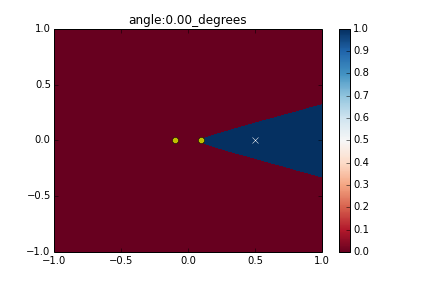
\includegraphics[width=\textwidth]{sim/sim_2_1}
    \caption{source at $(r=50$ cm, $\theta = 0$ degrees$)$}
  \end{subfigure}
  \begin{subfigure}[]{.23\textwidth}
    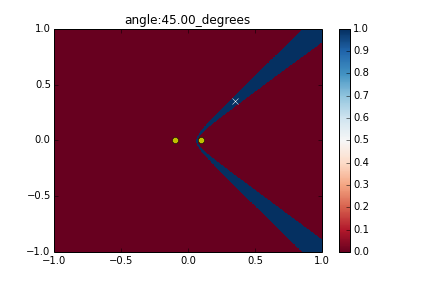
\includegraphics[width=\textwidth]{sim/sim_2_2}
    \caption{source at $(r=50$ cm, $\theta = 45$ degrees$)$}
  \end{subfigure}
  \begin{subfigure}[]{.23\textwidth}
    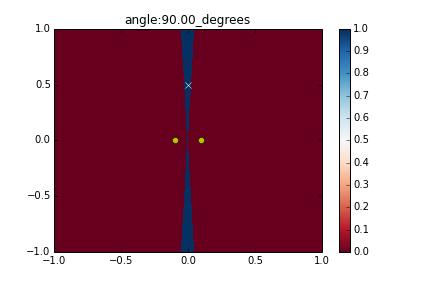
\includegraphics[width=\textwidth]{sim/sim_2_3}
    \caption{source at $(r=50$ cm, $\theta = 90$ degrees$)$}
  \end{subfigure}
  \caption{Uncertainty region. Yellow dots represent microphones' locations and the white dot represents the location of the source.}
  \label{fig:sim_2_5}
\end{figure}

To see how precision affects localization accuracy, we simulated two microphones placed at: $M_1:(x=-10\mbox{ cm},y=0\mbox{ cm})$ and $M_2:(x=10\mbox{ cm},y=0\mbox{ cm})$. A test sound source is emitted at point $P$ which is $50$ centimeters away from the origin $(0,0)$. Let $2a$ denote the difference of distance between $P$ and two microphones:
\[
2a = P M_1 - P M_2 
\]
, then fig~\ref{fig:sim_2_5} shows the region $R$ where all points have difference of distance to two microphones close to $2a$ within $1$ cm:
\[
R=\{\hat P: |(\hat P M_1 - \hat P M_2) - 2a|< 1 \mbox{ cm}\}
\]
Intuitively, points in $R$ have difference of distance to two microphones very similar to each other. Looking at fig~\ref{fig:sim_2_5}, we can still see that $R$ has the shape of a hyperbola, but with an uncertainty region around it. The thickness of the uncertainty region is not uniform around the hyperbola, the farther away the point is, the larger the uncertainty region becomes. This indicates for the same delta distance movement it will generate smaller difference of distance change when the source is farther away from the array. The size of the uncertainty region is also angle dependent: points closer to the line connecting microphones have larger region compared to points close to the line bisecting microphones. 

This can also be seen analytically. Assuming two microphones are placed on the x-axis at $M_1:(-c,0)$ and $M2:(c,0)$. All points $P:(x,y)$ with difference of distance $ |PM_1 - PM_2| = 2a$ satisfies:
\begin{eqnarray}\label{eqn:hyperbola}
\frac{x^2}{a^2} - \frac{y^2}{c^2-a^2} = 1
\end{eqnarray}
To see how the difference of distance changes with respect to source location, we can expand the equation and find the partial differential $\frac{\partial a}{\partial x}$:
\begin{eqnarray}\label{eqn:derivative}
\frac{\partial a}{\partial x} = \frac{x(c^2-a^2)}{a(x^2+y^2+c^2)-2a^3}
\end{eqnarray}
Since all points in equation~\ref{eqn:derivative} must lie on the hyperbola, we can substitute~\ref{eqn:hyperbola} into~\ref{eqn:derivative}:
\begin{eqnarray}\label{eqn:derivativeF}
\frac{\partial a}{\partial x} = \frac{c^2-a^2}{\frac{c^2}{a}x - \frac{a^3}{x}}
\end{eqnarray}

The denominator of equation~\ref{eqn:derivativeF} increases monotonically as $|x|$ increases, which indicates $\frac{\partial a}{\partial x}$ decreases as we move farther away along the hyperbola. The same distance move $\delta x$ would generate smaller change in difference of distance $a$ when the source is farther away from the microphones. 

\begin{figure*}[]
  \centering
  \begin{subfigure}[]{.3\textwidth}
    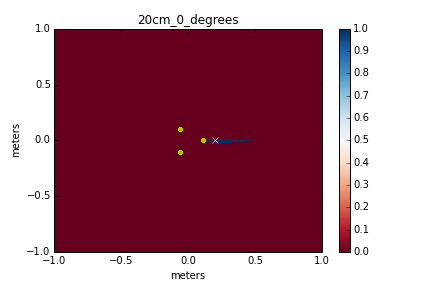
\includegraphics[width=\textwidth]{sim/result_20cm_0_degrees}
    \caption{0 degrees}
  \end{subfigure}
  \begin{subfigure}[]{.3\textwidth}
    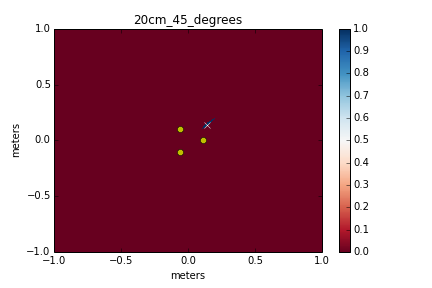
\includegraphics[width=\textwidth]{sim/result_20cm_45_degrees}
    \caption{45 degrees}
  \end{subfigure}
  \begin{subfigure}[]{.3\textwidth}
    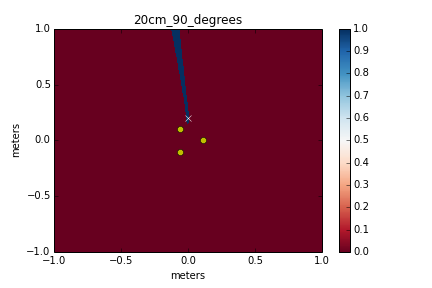
\includegraphics[width=\textwidth]{sim/result_20cm_90_degrees}
    \caption{90 degrees}
  \end{subfigure}
  \begin{subfigure}[]{.3\textwidth}
    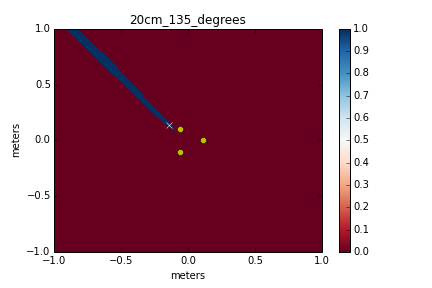
\includegraphics[width=\textwidth]{sim/result_20cm_135_degrees}
    \caption{135 degrees}
  \end{subfigure}
  \begin{subfigure}[]{.3\textwidth}
    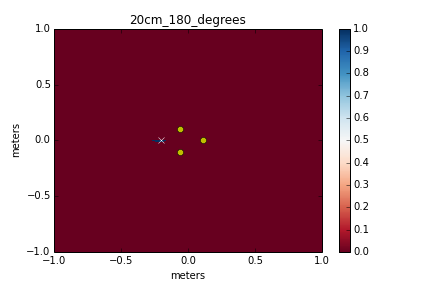
\includegraphics[width=\textwidth]{sim/result_20cm_180_degrees}
    \caption{180 degrees}
  \end{subfigure}
  \caption{Uncertainty region. Microphones are at the vertices of a $20$cm equilateral triangle. The source is $20$cm away from the array.}
  \label{fig:sim_3_2}
\end{figure*}

\begin{figure*}[]
  \centering
  \begin{subfigure}[]{.3\textwidth}
    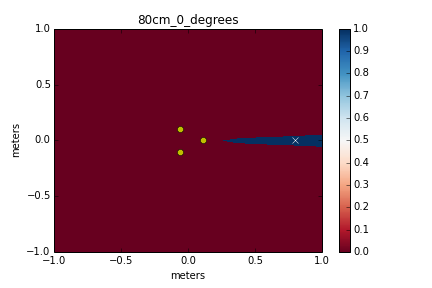
\includegraphics[width=\textwidth]{sim/result_80cm_0_degrees}
    \caption{0 degrees}
  \end{subfigure}
  \begin{subfigure}[]{.3\textwidth}
    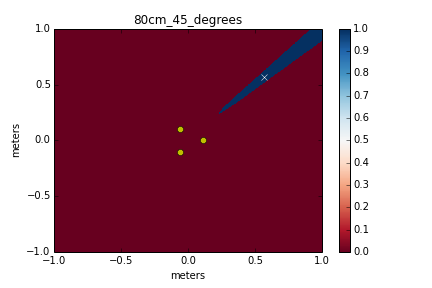
\includegraphics[width=\textwidth]{sim/result_80cm_45_degrees}
    \caption{45 degrees}
  \end{subfigure}
  \begin{subfigure}[]{.3\textwidth}
    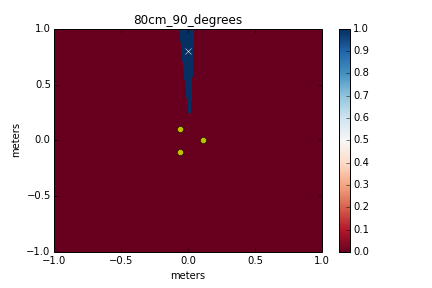
\includegraphics[width=\textwidth]{sim/result_80cm_90_degrees}
    \caption{90 degrees}
  \end{subfigure}
  \begin{subfigure}[]{.3\textwidth}
    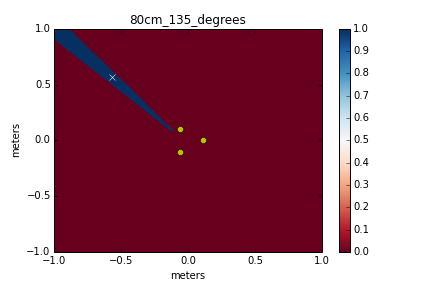
\includegraphics[width=\textwidth]{sim/result_80cm_135_degrees}
    \caption{135 degrees}
  \end{subfigure}
  \begin{subfigure}[]{.3\textwidth}
    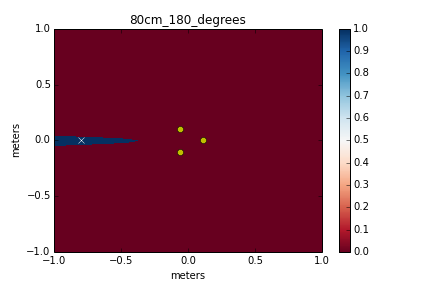
\includegraphics[width=\textwidth]{sim/result_80cm_180_degrees}
    \caption{180 degrees}
  \end{subfigure}
  \caption{Uncertainty region. Microphones are at the vertices of a $20$cm equilateral triangle. The source is $80$cm away from the array.}
  \label{fig:sim_3_8}
\end{figure*}

With more than two microphones, each pair of microphones generates a hyperbolic region and localization becomes finding the intersection of hyperbolic regions. The smaller the intersection region, the better the localization accuracy. To see how accuracy changes with array placement and sound source location, three microphones are placed at the three vertices of a $20$ cm equilateral triangle. An audio source is placed at $20$ cm away from the center of the array. Fig~\ref{fig:sim_3_2} shows the intersection of regions for $5$ different placement of the sound source. It can be seen that accuracy decreases when sound source becomes close to the line connecting any two microphones. This observation is consistent with the two microphone case, since points close to lines connecting microphones have a larger uncertainty region.

To see how sound source distance affects localization accuracy, the same simulation is carried out with the sound source moved from $20$ cm to $80$ cm away from the center of the array. Results are presented in fig~\ref{fig:sim_3_8}. Comparing with fig~\ref{fig:sim_3_2}, accuracy decreases as the distance to the array increases. This is also consistent with our observation in $2$ microphone case where sources farther away would result in larger uncertainty region.

\begin{figure*}[]
  \centering
  \begin{subfigure}[]{.3\textwidth}
    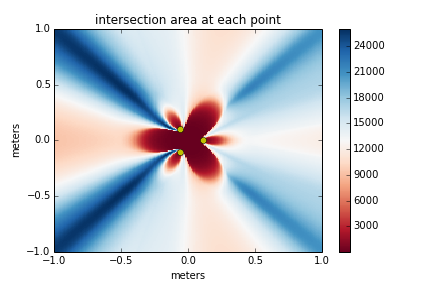
\includegraphics[width=\textwidth]{sim/result_intersection_area_at_each_point_3_center}
    \caption{$3$ microphones are placed at vertices of a $20$cm equilateral triangle. The average error is $18.6$ cm}
    \label{fig:sim_hm_3}
  \end{subfigure}
  \begin{subfigure}[]{.3\textwidth}
    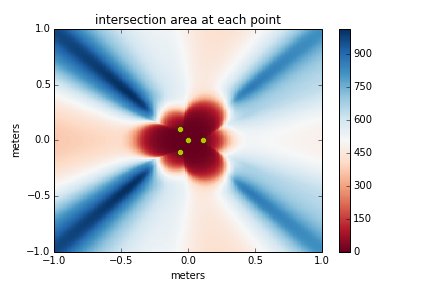
\includegraphics[width=\textwidth]{sim/result_intersection_area_at_each_point_3_p1}
    \caption{Another microphone is added at origin. The average error is $17.1$ cm}
    \label{fig:sim_hm_3_p1}
  \end{subfigure}
  \begin{subfigure}[]{.3\textwidth}
    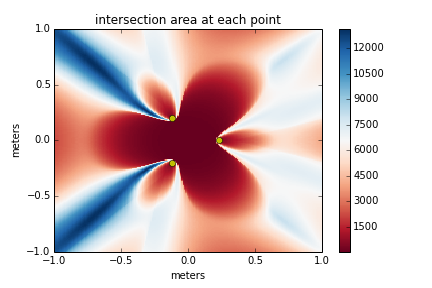
\includegraphics[width=\textwidth]{sim/result_intersection_area_at_each_point_3_2x}
    \caption{$3$ microphones are placed at vertices of a $40$cm equilateral triangle. The average error is $10.04$ cm}
    \label{fig:sim_hm_3_2x}
  \end{subfigure}
  \begin{subfigure}[]{.3\textwidth}
    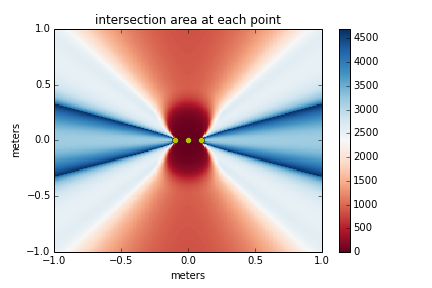
\includegraphics[width=\textwidth]{sim/result_intersection_area_at_each_point_3_line}
    \caption{$3$ microphones are placed in a line, $10$ cm apart from each other. The average error is $55.05$ cm}
    \label{fig:sim_hm_3_line}
  \end{subfigure}
  \begin{subfigure}[]{.3\textwidth}
    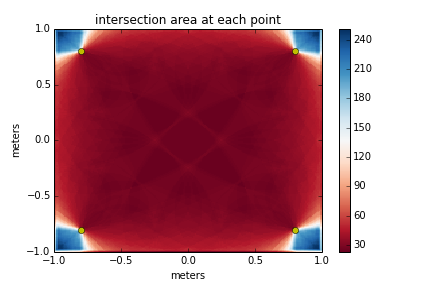
\includegraphics[width=\textwidth]{sim/result_intersection_area_at_each_point_4corner}
    \caption{$4$ microphones are placed at $4$ corners of the grid. The average error is $0.05$ cm}
    \label{fig:sim_hm_4}
  \end{subfigure}
  \begin{subfigure}[]{.3\textwidth}
    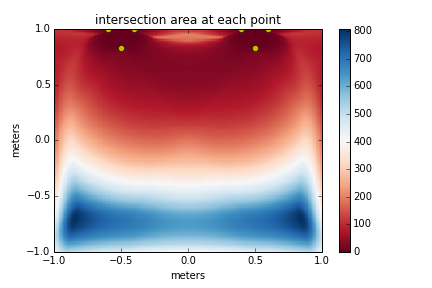
\includegraphics[width=\textwidth]{sim/result_intersection_area_at_each_point_2a}
    \caption{Two $3$ microphone arrays are placed $1$ meter apart. The average error is $2.60$ cm}
    \label{fig:sim_hm_2_array}
  \end{subfigure}
  \caption{Error heatmap for different array configurations}
  \label{fig:sim_hm}
\end{figure*}

Each microphone pair generates a hyperbolic region, and the source location is in the intersection of these regions. The area of the intersection region is a measure of the localization accuracy: the smaller the area, the more certain we are about the source location. To evaluate an array's accuracy in a region, we can place sound source at predetermined grid points in the region and look at the intersection area for each tested point in the grid. The center location of the intersection region can be used as the localization estimate to calculate localization error. Results for a few different microphone array configurations are presented in fig~\ref{fig:sim_hm}.

Fig~\ref{fig:sim_hm_3} shows the accuracy when microphones are placed at the three vertices of a $20$ cm equilateral triangle. The region inside the array has good accuracy. However, for regions along the line connecting any two microphones, the accuracy drops significantly. The average error across the region is $18.6$ cm.

To evaluate how adding one microphone(without increasing the array size) improves accuracy, another microphone is added to the array at $(0,0)$. Result is presented in fig~\ref{fig:sim_hm_3_p1}. Addition of the new microphone only slightly improved the accuracy around the array region. The average error dropped from $18.6$ cm to $17.1$ cm. Regions near lines connecting microphones still have significantly larger uncertainty region.

To evaluate the array size's impact on accuracy, the size of the original array (as in fig~\ref{fig:sim_hm_3}) is increased by a factor of $2$. The result is presented in fig~\ref{fig:sim_hm_3_2x}. The overall uncertainty area decreased across the region. The average error improved to $10.04$ cm. 

In fig~\ref{fig:sim_hm_3_line}, three microphones are placed $10$ cm apart from each other on the x-axis. Error heatmap shows high uncertainty on the x axis, and the overall accuracy is not as good as that with three microphones placed in a triangle. The average error is $55.05$ cm. 

To further increase the distance between microphones, we placed four microphones at four corners of the region. Fig~\ref{fig:sim_hm_4} shows the result. With this configuration, accuracy is consistently good across the region. The average error is $0.05$ cm.  However, placing microphones far apart at corners of the region requires accurate placement of all four individual microphones. The system is less portable compared to small arrays with microphones near each other. Placing microphones far apart from each other also causes problems in TDOA estimation, because sampling of microphones in the same array requires synchronized clock.

To avoid the need to accurately place microphones at far distances(as required by fig~\ref{fig:sim_hm_4}), we explored configuration with two arrays. Two $3$ microphone array are placed $1$ meter apart and the result is presented in fig~\ref{fig:sim_hm_2_array}.  The result indicates that this configuration has good accuracy when source is close to the arrays. Accuracy decreases as sound source moves outside of the one meter by one meter region. The average error is $2.60$ cm. 

With the simulation results, we decided to build the two array system as described in fig~\ref{fig:sim_hm_2_array}. The setup is reasonably portable (compared to fig~\ref{fig:sim_hm_4}), while at the same time having significantly better accuracy compared to one array systems.

\subsection{Hardware}
The end system has two arrays, each with three microphones mounted on the vertices of a $20$ cm equilateral triangle. We used omni-directional foil electret condenser microphone due to its low cost and small size. The microphone has a frequency range of $100$ to $10K$ Hz, and a minimum SNR of 58dB\cite{sys:1}. We also used operational amplifer OPA344 from Texas Instrument to amplify the microphone output by a factor of 100, so the received signal can be easily picked up by the analog-to-digital converter (ADC) module installed on the micro-controller. The micro-controller board used in this project is \emph{teensy 3.1}, and it is attached to one of the vertices of the triangle. Fig~\ref{fig:setup_array} shows a picture of the array setup.  The micro-controller contains an onboard RAM of $64$k, and an ADC module capable of sampling at $500$kHz~\cite{tdoa:micloc, sys:teensy}. In this project, the micro-controller collects microphone data on all three channels for a duration $12$ milliseconds and then sends the recorded data to a computer through the USB port for localization. 

\begin{figure}[h!]
  \centering
  \begin{subfigure}[]{.48\textwidth}
    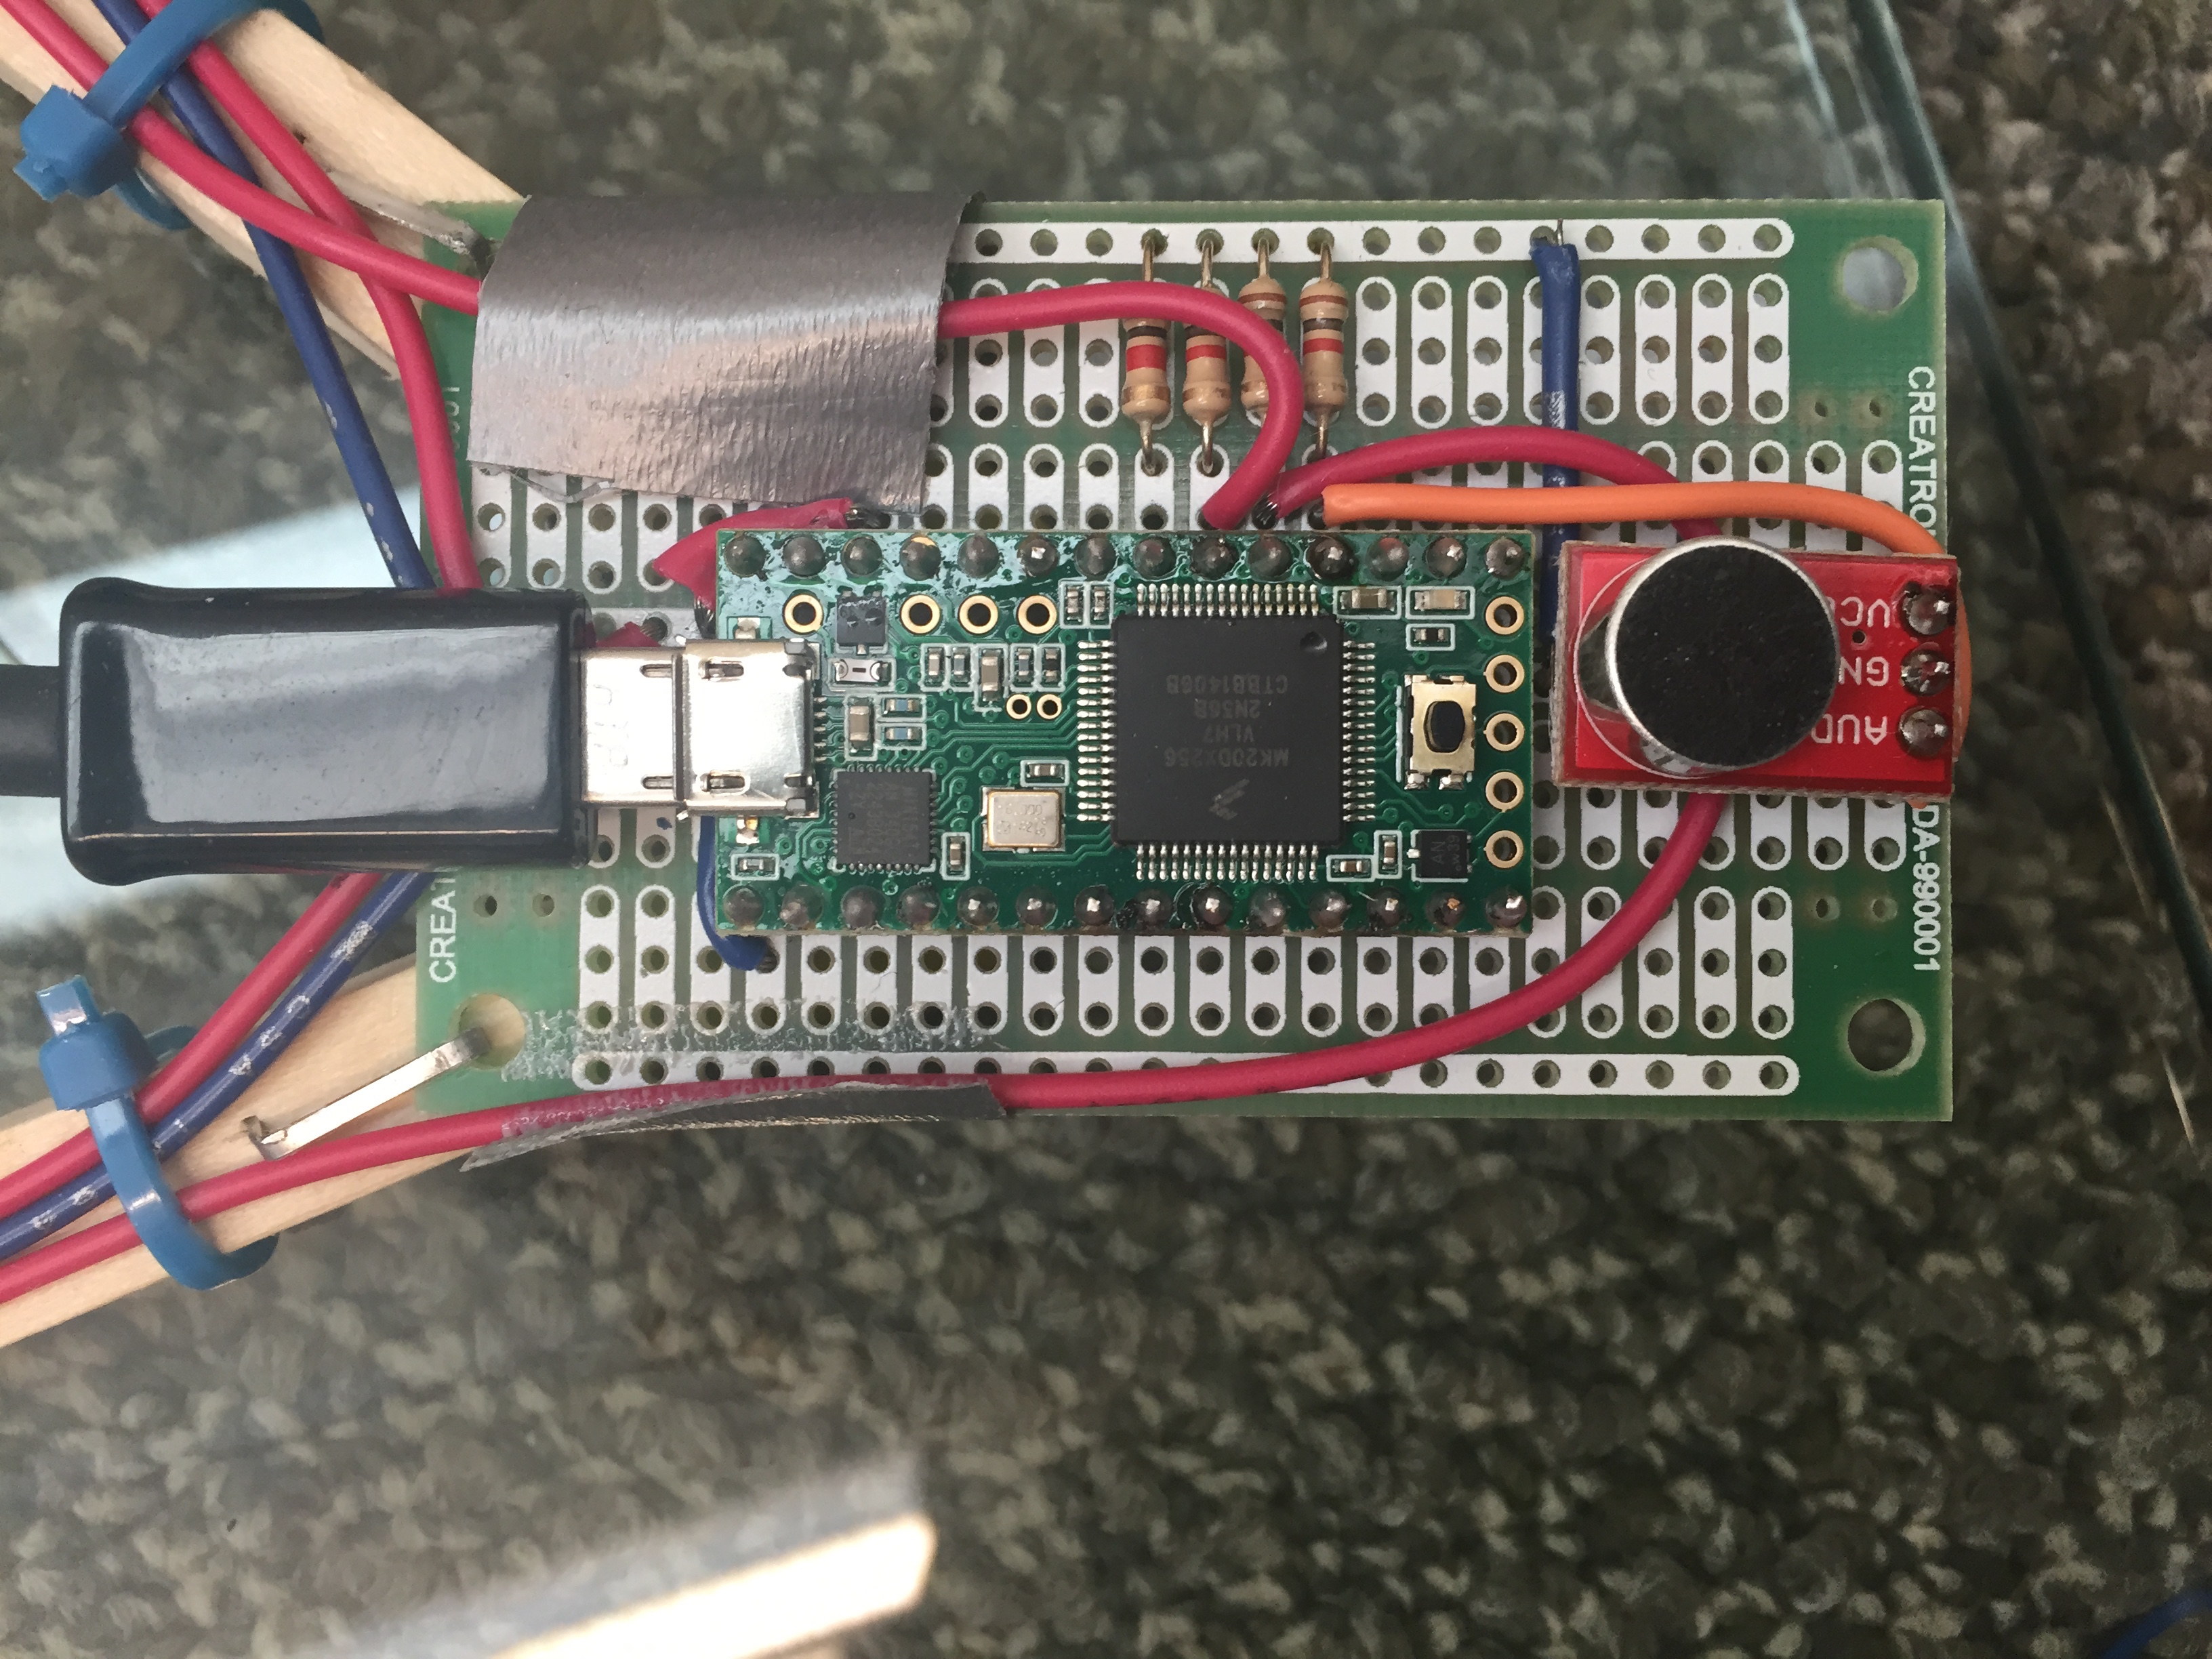
\includegraphics[width=\textwidth]{array_close.JPG}
    \caption{micro-controller}
  \end{subfigure}
  \begin{subfigure}[]{.48\textwidth}
    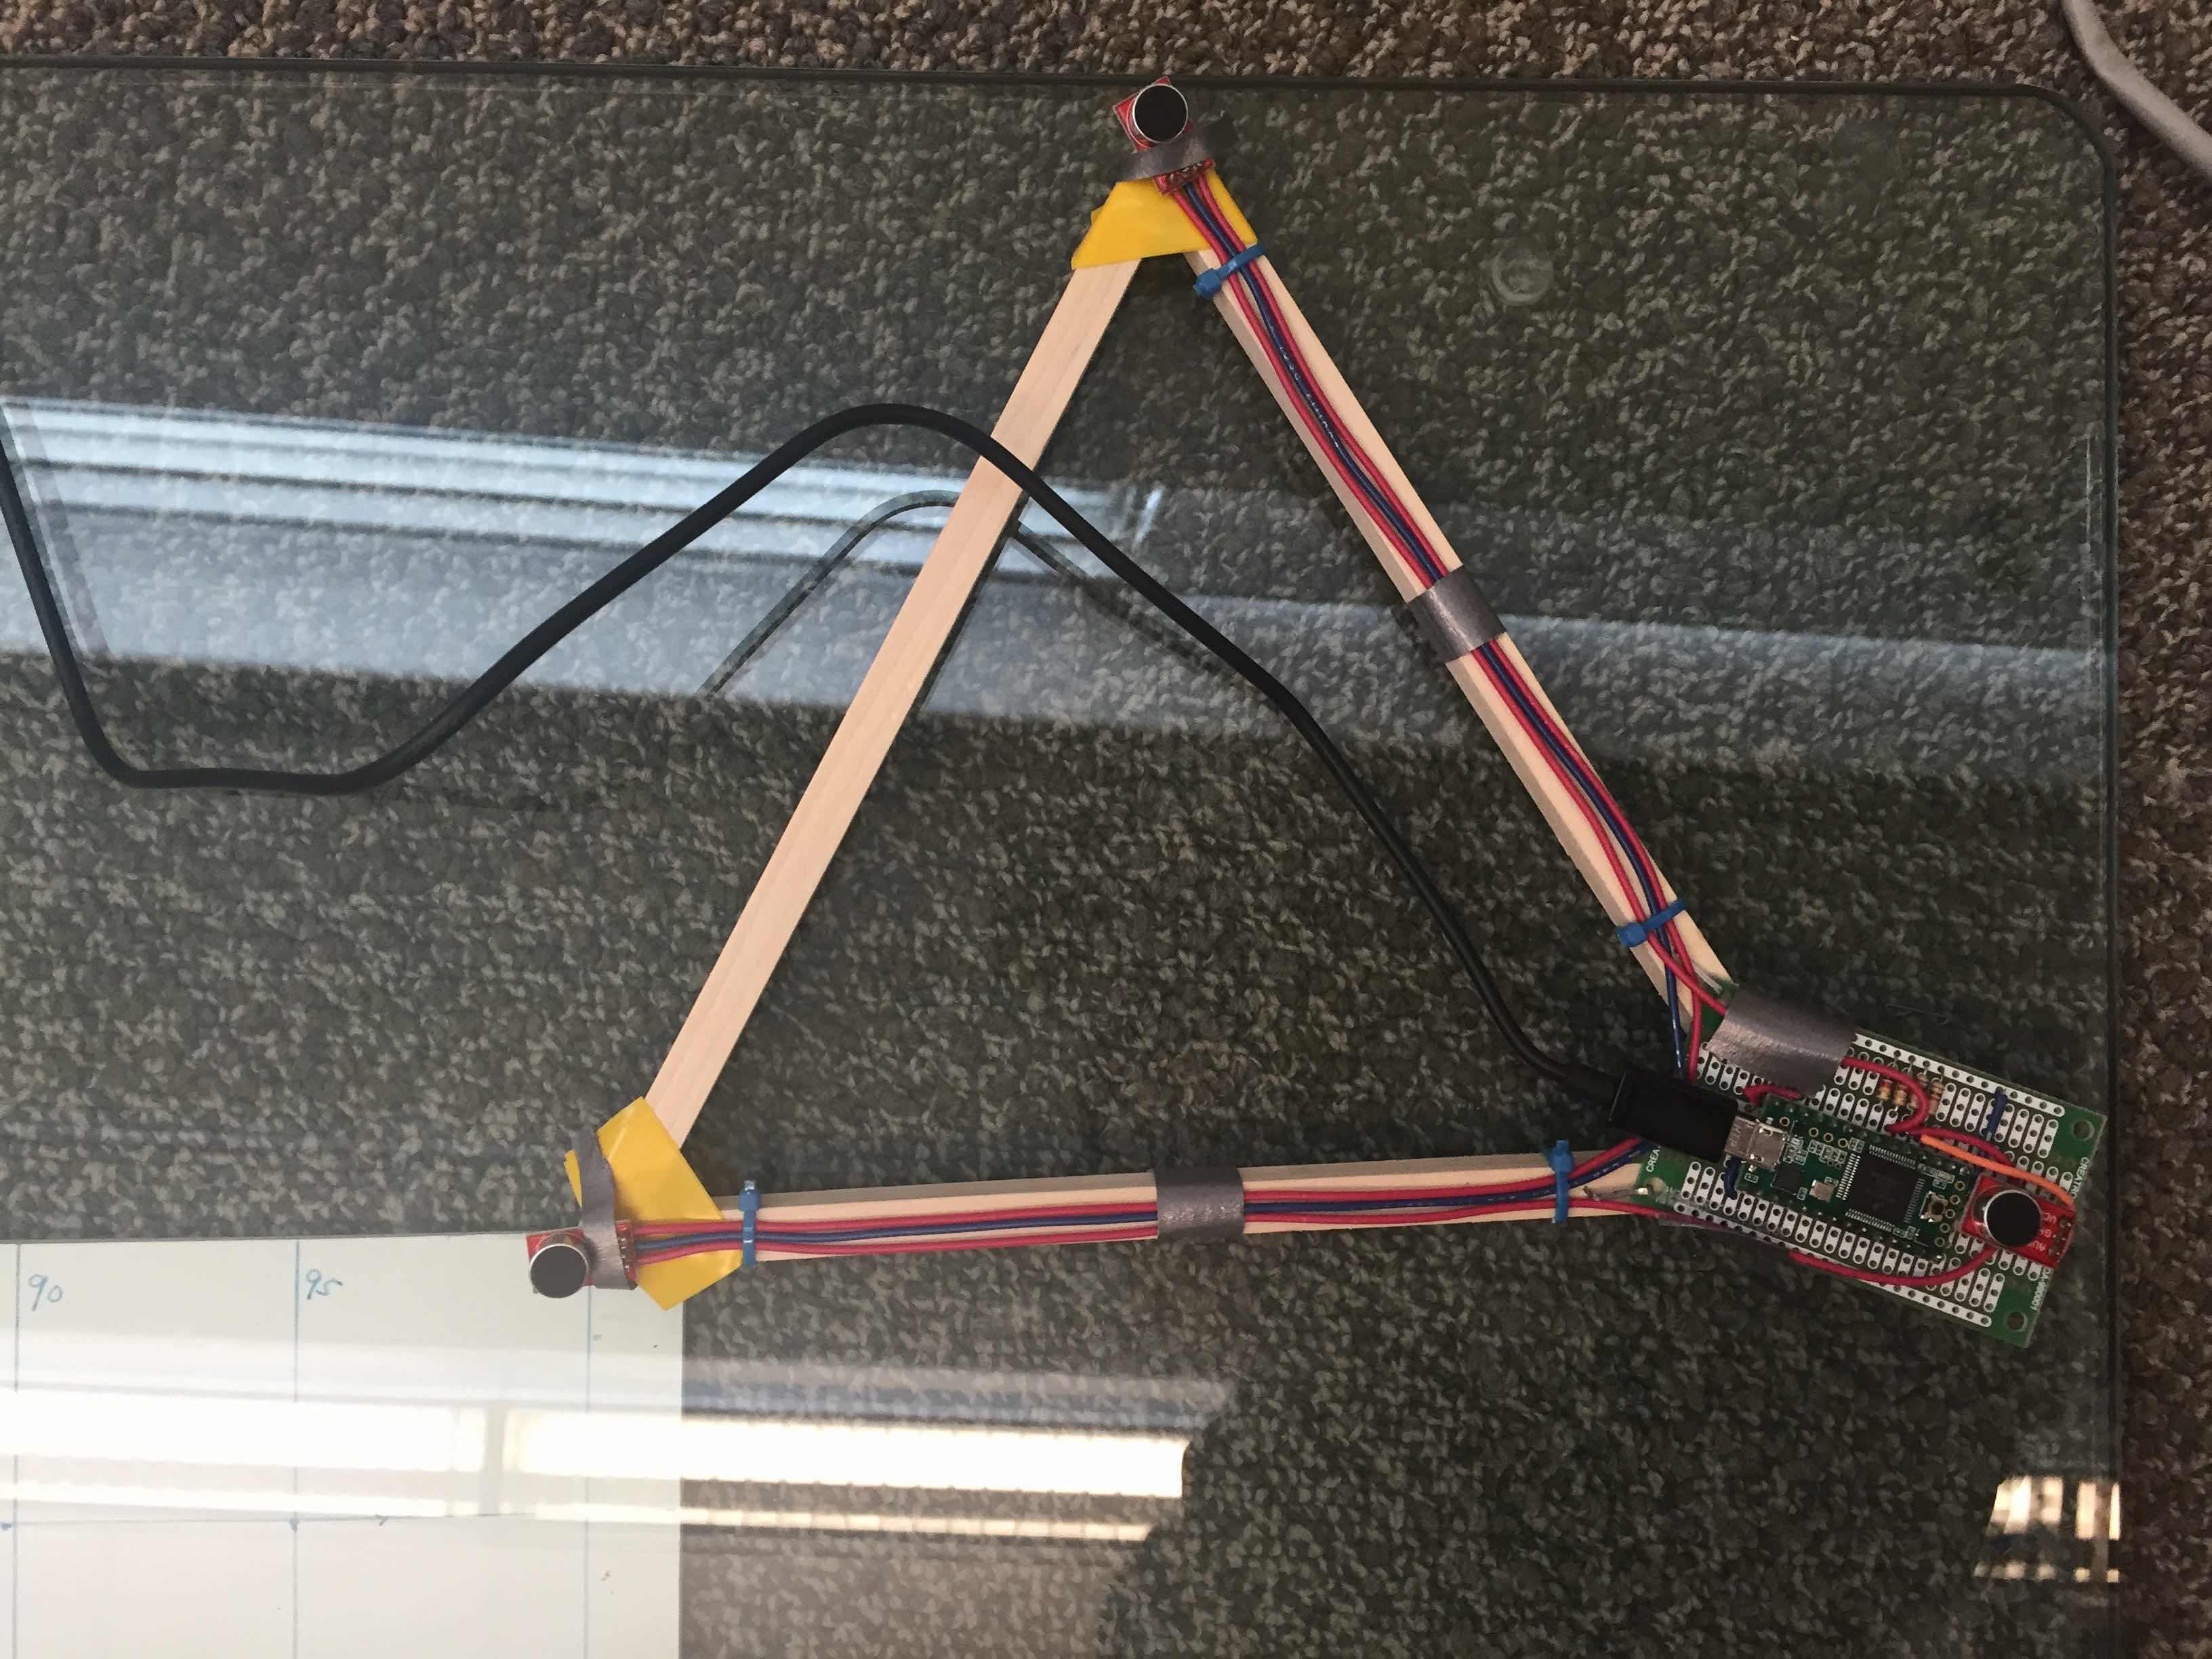
\includegraphics[width=\textwidth]{array.JPG}
    \caption{array}
  \end{subfigure}
  \begin{subfigure}[]{.48\textwidth}
    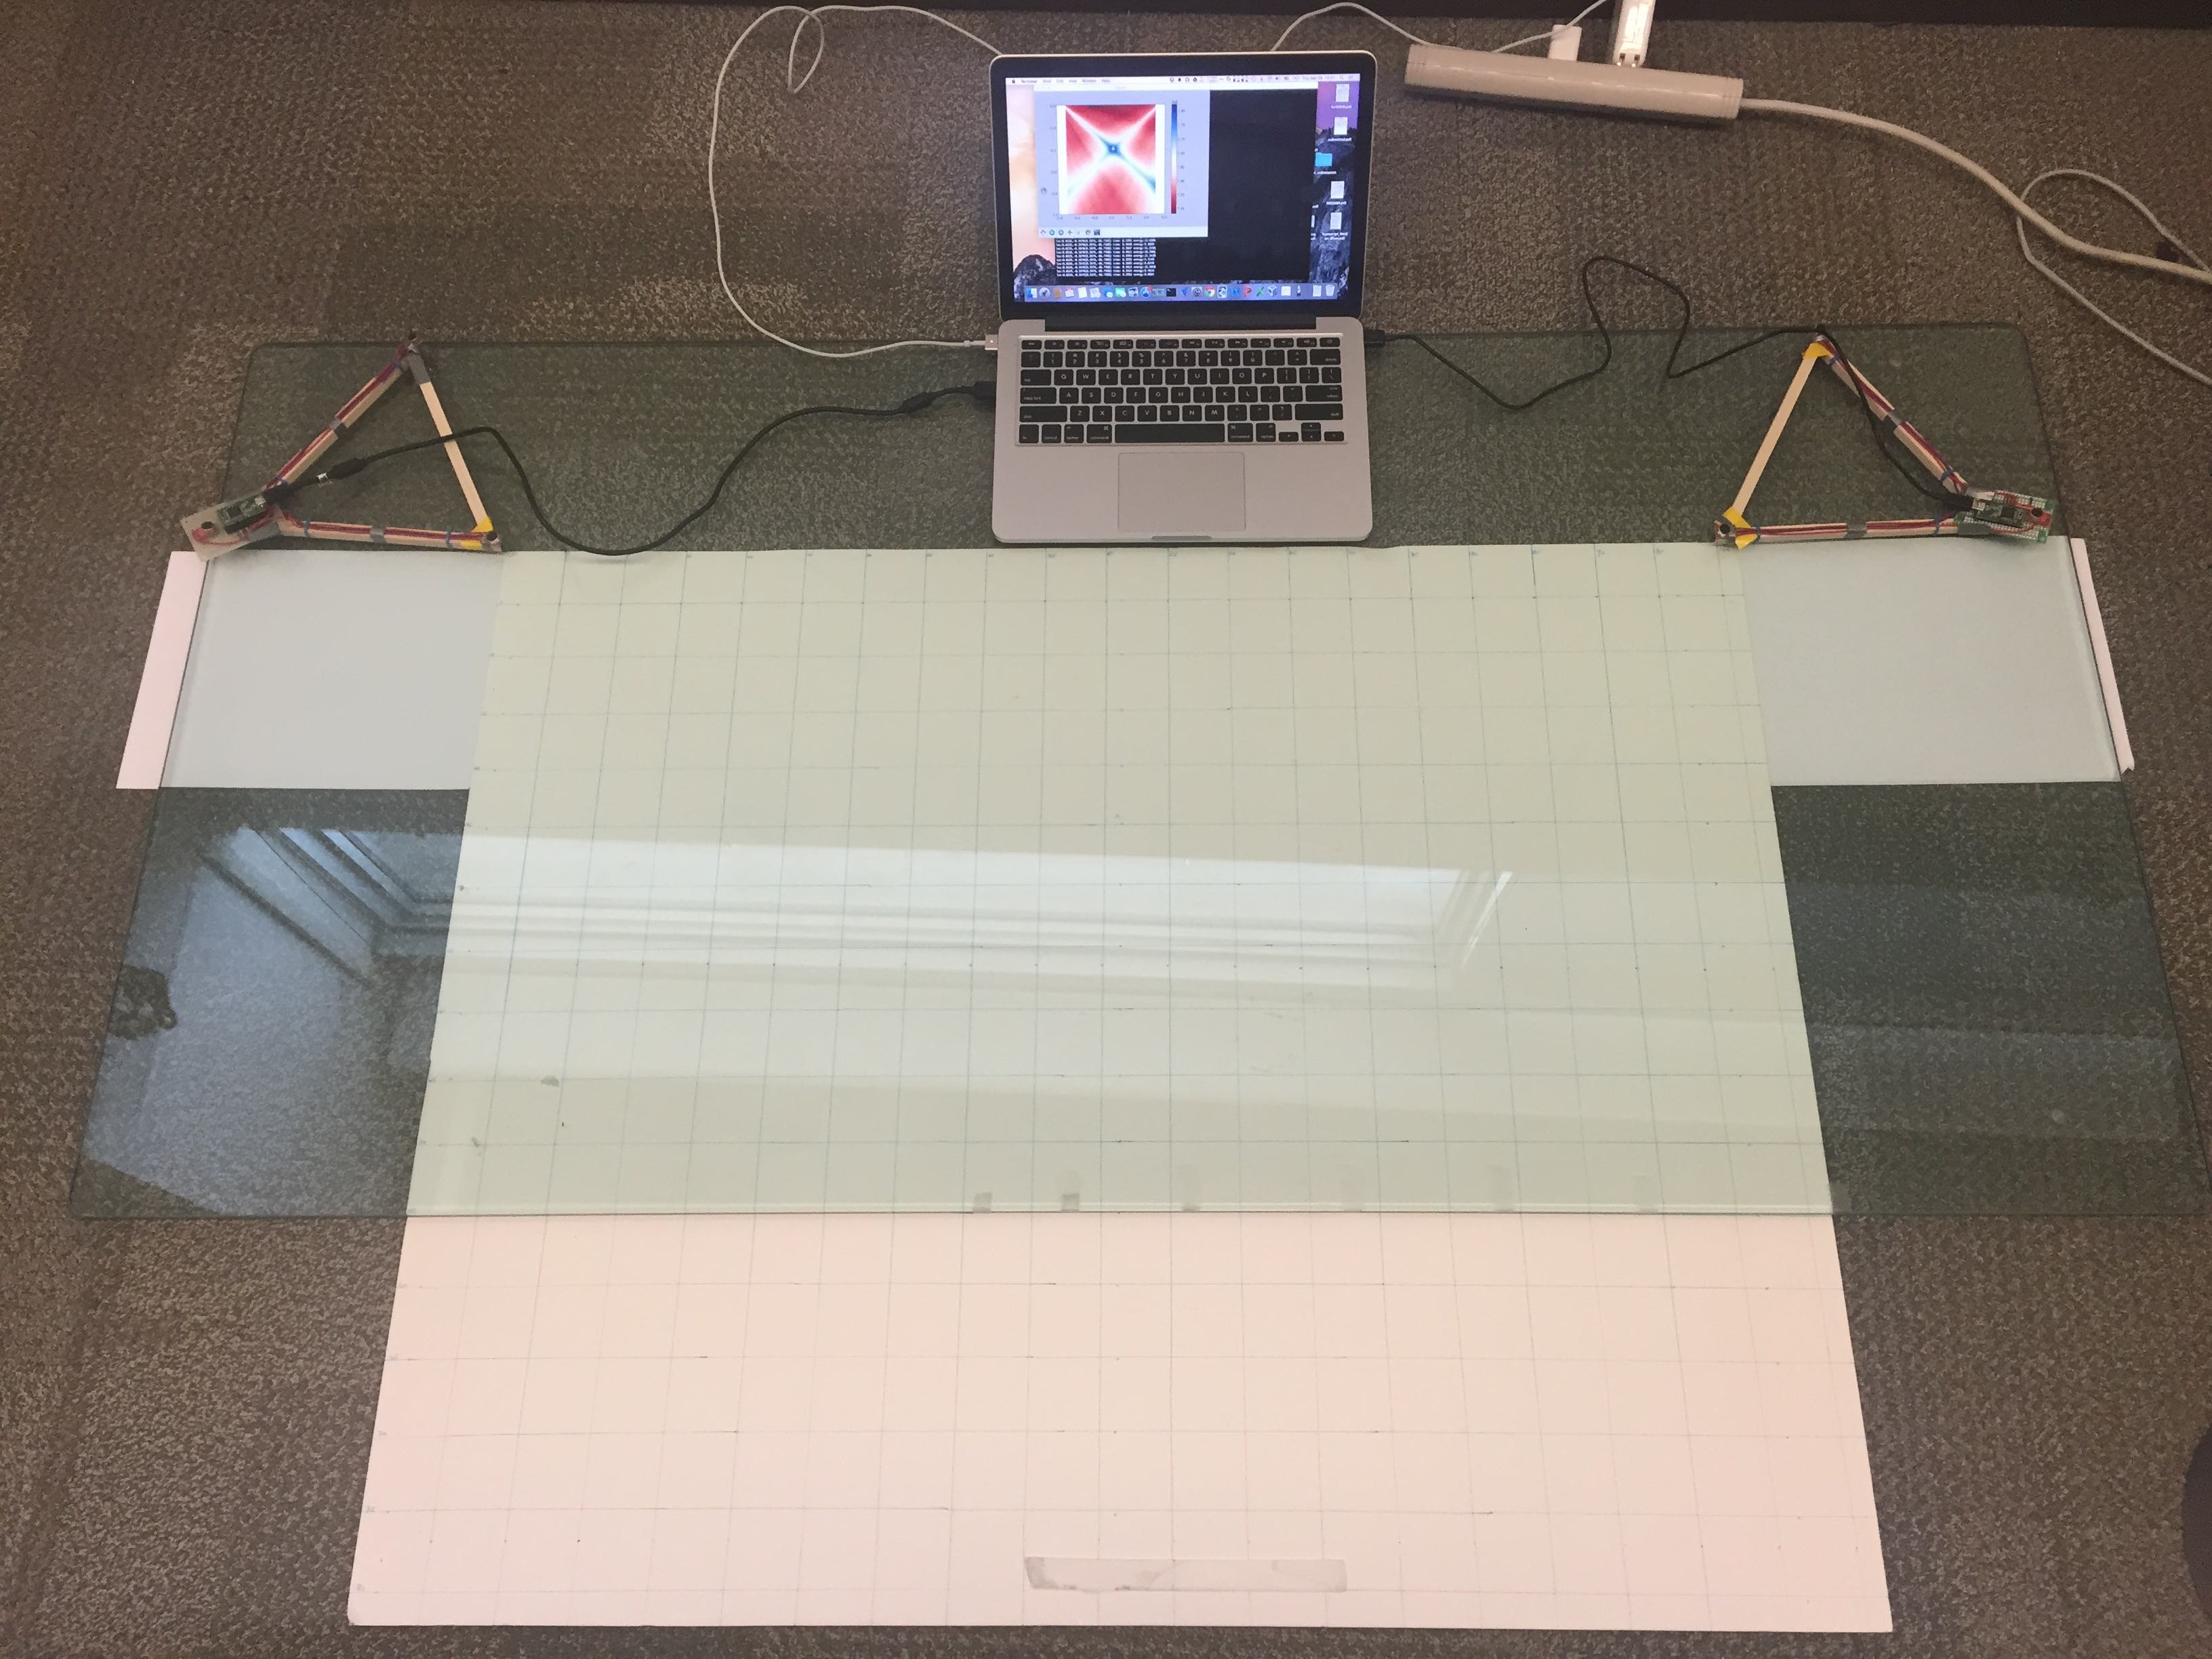
\includegraphics[width=\textwidth]{setup_2.JPG}
    \caption{two arrays}
  \end{subfigure}
  \caption{Localization system setup}
  \label{fig:setup_array}
\end{figure}

\subsection{Software}

On the software side, \emph{Python} is used as the main programming language since it has extensive libraries in both real time data handling and signal processing. \emph{ZeroMQ} is an inter process messaging queue that is used in our system to pass data across different modules. Our system is made up of two data acquisition modules (each is used to receive raw date from microphone array output) and one localization module (listens to both data acquisition modules and perform localization using the raw microphone data). Using ZeroMQ as connections to different modules adds flexibility to our system, as we can design applications such as the drawing application we have used in our system to interface only with the localization module and disregard how the microphone data is collected. Other localization applications can be easily integrated into our system by connecting them with the localization module. Furthermore, we have built a recording module that interfaces with the data acquisition modules for offline analysis and parameter tuning. 

To handle the uncertainty in TDOA estimation, instead of using point estimate that maximizes equation~\ref{eq:gcc}, we take the cross-correlation output(equation~\ref{eq:gcc2}) as a measure of the likelihood of different arrival time differences. Each index $i$ from the cross-correlation vector denotes the time delay across the two microphones receiving the acoustic signal, and the cross-correlation value $k$[i] at each index $i$ denotes the likelihood of the time delay being $i$. 

For each microphone array, we build a heatmap of likelihood for the region. The intensity at each point on the heatmap represents the likelihood of it being the source. To generate the likelihood heatmap for an microphone array, we apply the following algorithm. For each point ($x$,$y$) on the grid, the theoretical TDOA to each microphone pair can be precomputed using:
\[
 D_{m_1,m_2}(x,y) =  \frac{((x-x_1)^2 + (y-y_1)^2)^{0.5} - ((x-x_2)^2 + (y-y_2)^2)^{0.5}}{v}
\]
where ($x_1, y_1$) and ($x_2, y_2$) are the locations of the microphone pair and $v$ is the speed of sound. Then the heatmap can be generated by going through all the points on the grid and performing a lookup using equation~\ref{eq:gcc2}. With three microphones $m_1,m_2,$ and $m_3$, there are three microphone pairs: $m_1m_2,m_1m_3,$ and $m_2m_3$. The theoretical TDOA from each location $(x,y)$ to each microphone pair is precomputed and stored in $D_{m_1,m_2}(x,y)$, $D_{m_1,m_3}(x,y)$, and $D_{m_2,m_3}(x,y)$. Then the likelihood map $L(x,y)$ can be built by superposing the likelihood from each microphone pair:
\begin{eqnarray*}
L(x,y) &=& R_{m_1,m_2}(D_{m_1,m_2}(x,y)) + R_{m_1,m_3}(D_{m_1,m_3}(x,y)) \\
 & & +R_{m_2,m_3}(D_{m_2,m_3}(x,y)) 
\end{eqnarray*}
where $R_{m_1,m_2}(\tau)$,$R_{m_1,m_3}(\tau)$, and $R_{m_2,m_3}(\tau)$ denote GCC output from microphone pairs $m_1m_2,m_1m_3,$ and $m_2m_3$.

Likelihood maps from two arrays can be combined into the final likelihood map:
\begin{equation}\label{eq:combine_l}
L(x,y) = L_1(x,y) L_2(x,y)
\end{equation}
where $L_1(x,y)$ and $L_2(x,y)$ represent the likelihood map from array $1$ and array $2$.

\begin{figure}[h!]
  \centering
  \begin{subfigure}[]{.48\textwidth}
    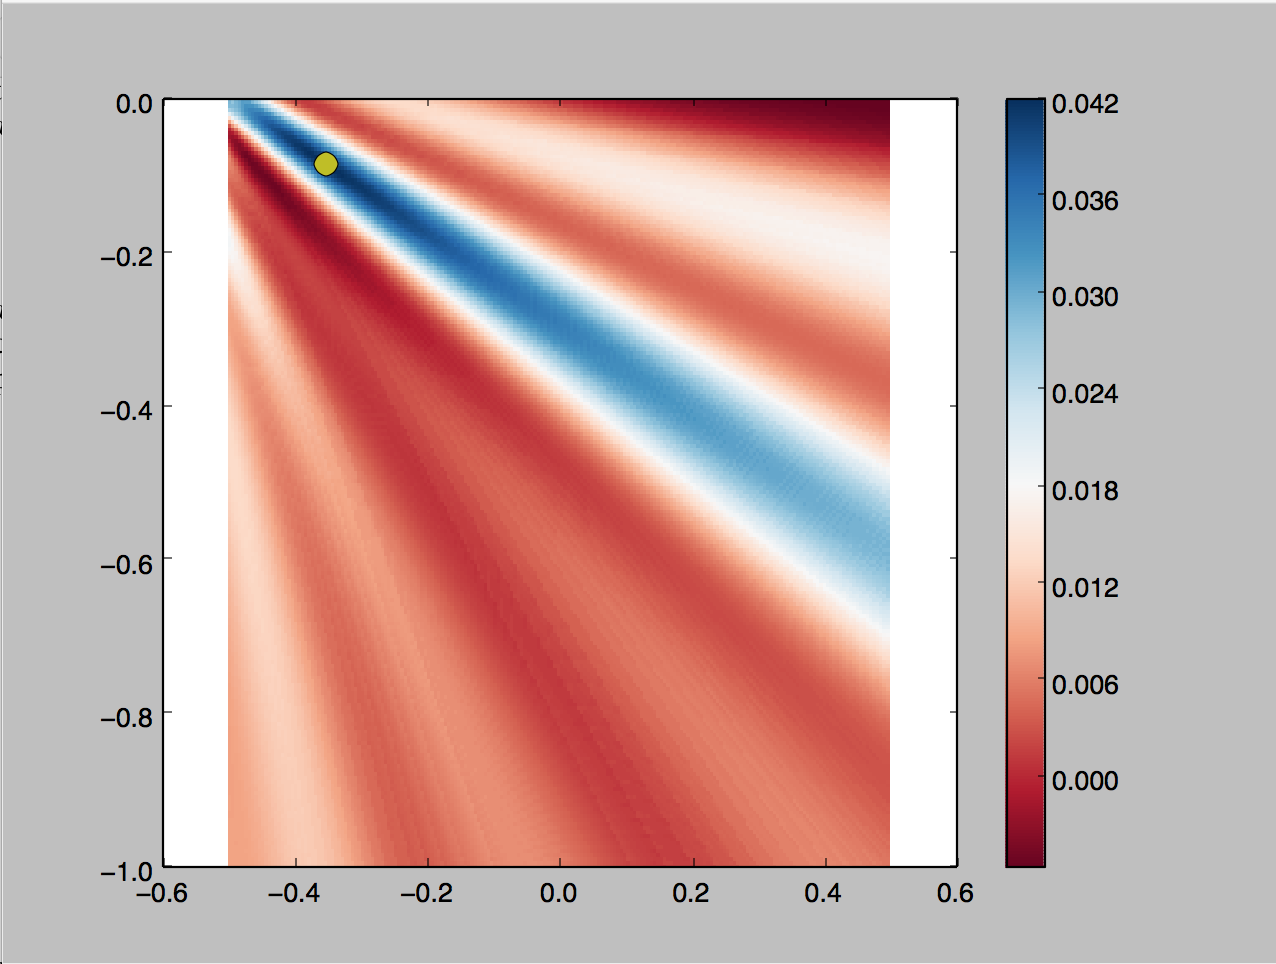
\includegraphics[width=\textwidth]{left.png}
    \caption{localization with only array 1}
    \label{fig:liklihood1}
  \end{subfigure}
  \begin{subfigure}[]{.48\textwidth}
    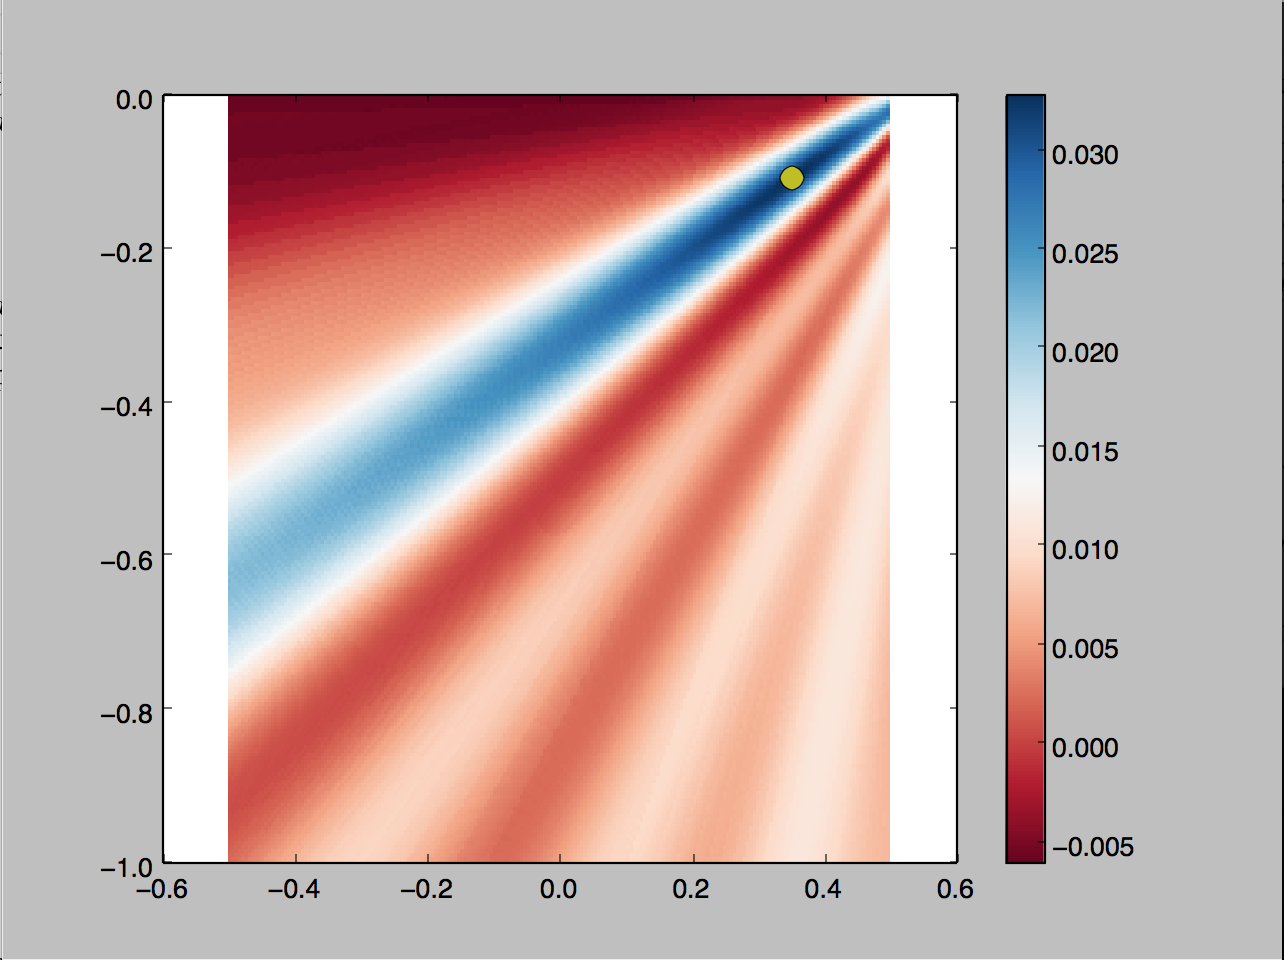
\includegraphics[width=\textwidth]{right.png}
    \caption{localization with only array 2}
    \label{fig:liklihood2}
  \end{subfigure}
  \begin{subfigure}[]{.48\textwidth}
    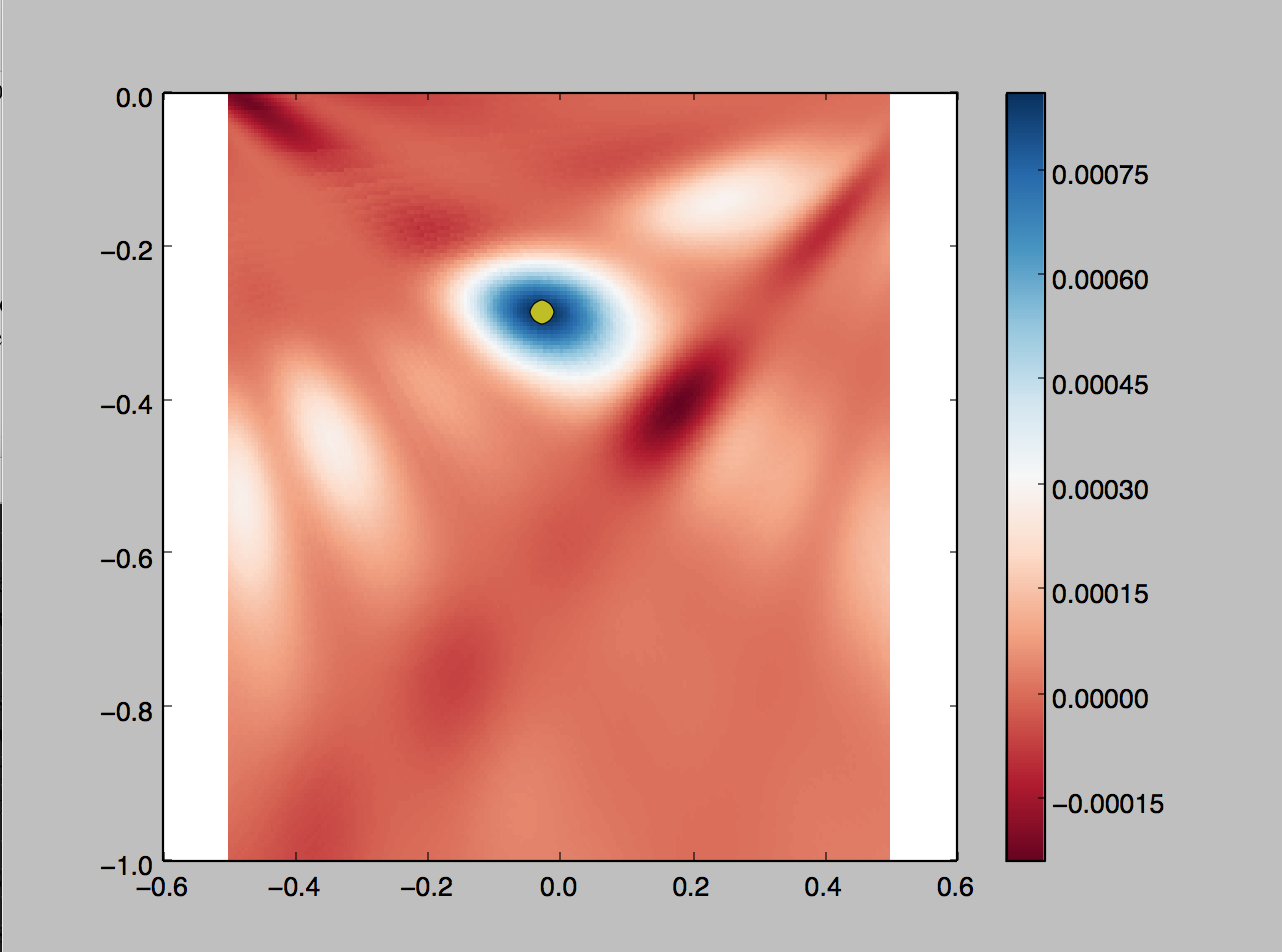
\includegraphics[width=\textwidth]{combined.png}
    \caption{localization with both arrays}
    \label{fig:liklihood3}
  \end{subfigure}
  \caption{Likelihood maps for localization. The source is placed at $(0.0,-0.3)$ m}
  \label{fig:liklihood}
\end{figure}

To see the effect of accuracy improvement using multiple arrays, fig~\ref{fig:liklihood} shows a real life localization where the source is placed at $(0$ cm$,-30$ cm$)$. The top two figures show the individual likelihood maps produced by single microphone arrays. We can see that the individual arrays can give accurate angle estimate, but have high uncertainty in distance estimate. The bottom figure shows the combined likelihood map according to equation~\ref{eq:combine_l}. The combined likelihood map demonstrated that by merging estimates from two arrays the system is able to perform more accurate localization. 


From a timing point of view, the micro-controller spends $12$ milliseconds on sampling the microphone data before sending it to a computer for processing. Sending the data through the USB port takes another $15$ milliseconds, and processing on the computer takes around $50$ milliseconds. Therefore, the total time lag between sound source and localization is around $80$ milliseconds.

\section{Sound Localization}
Points with the same time difference of arrival(TDOA) to two fixed points on a plane form a hyperbola. Since TDOA from each pair of microphones gives a hyperbola in the plane, localization becomes finding intersection of hyperbolas when more than two microphones are used. Localization relies on accurate estimate of delay differences between microphones.

Generalized Cross Correlation(GCC) provides a framework to estimate delay differences $t_0$ between two signals $x_1(t)$ and $x_2(t)$:
\begin{eqnarray} \label{eq:gcc}
t_0 &=& \arg\max_{\tau} R_{x_1x_2}(\tau) \\
R_{x_1x_2}(\tau) &=& \int_{-\infty}^\infty W(\omega) X_1(\omega) X_2^{*}(\omega) e^{j\omega\tau} d\omega
\end{eqnarray}
, where $X_1(\omega)$ and $X_2(\omega)$ are Fourier Transform of $x_1(t)$ and $x_2(t)$. $W(\omega)$ provides a way to prefilter signals passed to cross correlation estimator. We experimented with three ways of prefiltering the signal:
\begin{description}[\IEEEsetlabelwidth{Very very long label}\IEEEusemathlabelsep]
\item[GCC] $W(\omega) = 1$. No prefiltering is done. This is normal cross correlation.
\item[GCC\_PHAT] $W(\omega) = \frac{1}{\left|X_1(\omega)X_2^{*}(\omega)\right|}$. Each frequency is divideded by its magnitude. Only phase information contributes to delay estimation.
\item[GCC\_PHAT\_SQRT] $W(\omega) = \frac{1}{\left|X_1(\omega)X_2^*(\omega)\right|^{0.5}}$. This is somewhere between GCC and GCC\_PHAT. part of magnitude information is included in delay estimation.
\end{description}

\chapter{Experiment}
\section{System}
\subsection{Hardware}
The end system has two arrays, each with three microphones mounted on the vertices of a $20$ cm equilateral triangle. We used omni-directional foil electret condenser microphone due to its low cost and small size. The microphone has a frequency range of $100$ to $10K$ Hz, and a minimum SNR of 58dB\cite{sys:1}. We also used operational amplifer OPA344 from Texas Instrument to amplify the microphone output by a factor of 100, so the received signal can be easily picked up by the analog-to-digital converter (ADC) module installed on the micro-controller. The micro-controller board used in this project is \emph{teensy 3.1}, and it is attached to one of the vertices of the triangle. Fig~\ref{fig:setup_array} shows a picture of the array setup.  The micro-controller contains an onboard RAM of $64$k, and an ADC module capable of sampling at $500$kHz~\cite{tdoa:micloc, sys:teensy}. In this project, the micro-controller collects microphone data on all three channels for a duration $12$ milliseconds and then sends the recorded data to a computer through the USB port for localization. 

\begin{figure}[h!]
  \centering
  \begin{subfigure}[]{.48\textwidth}
    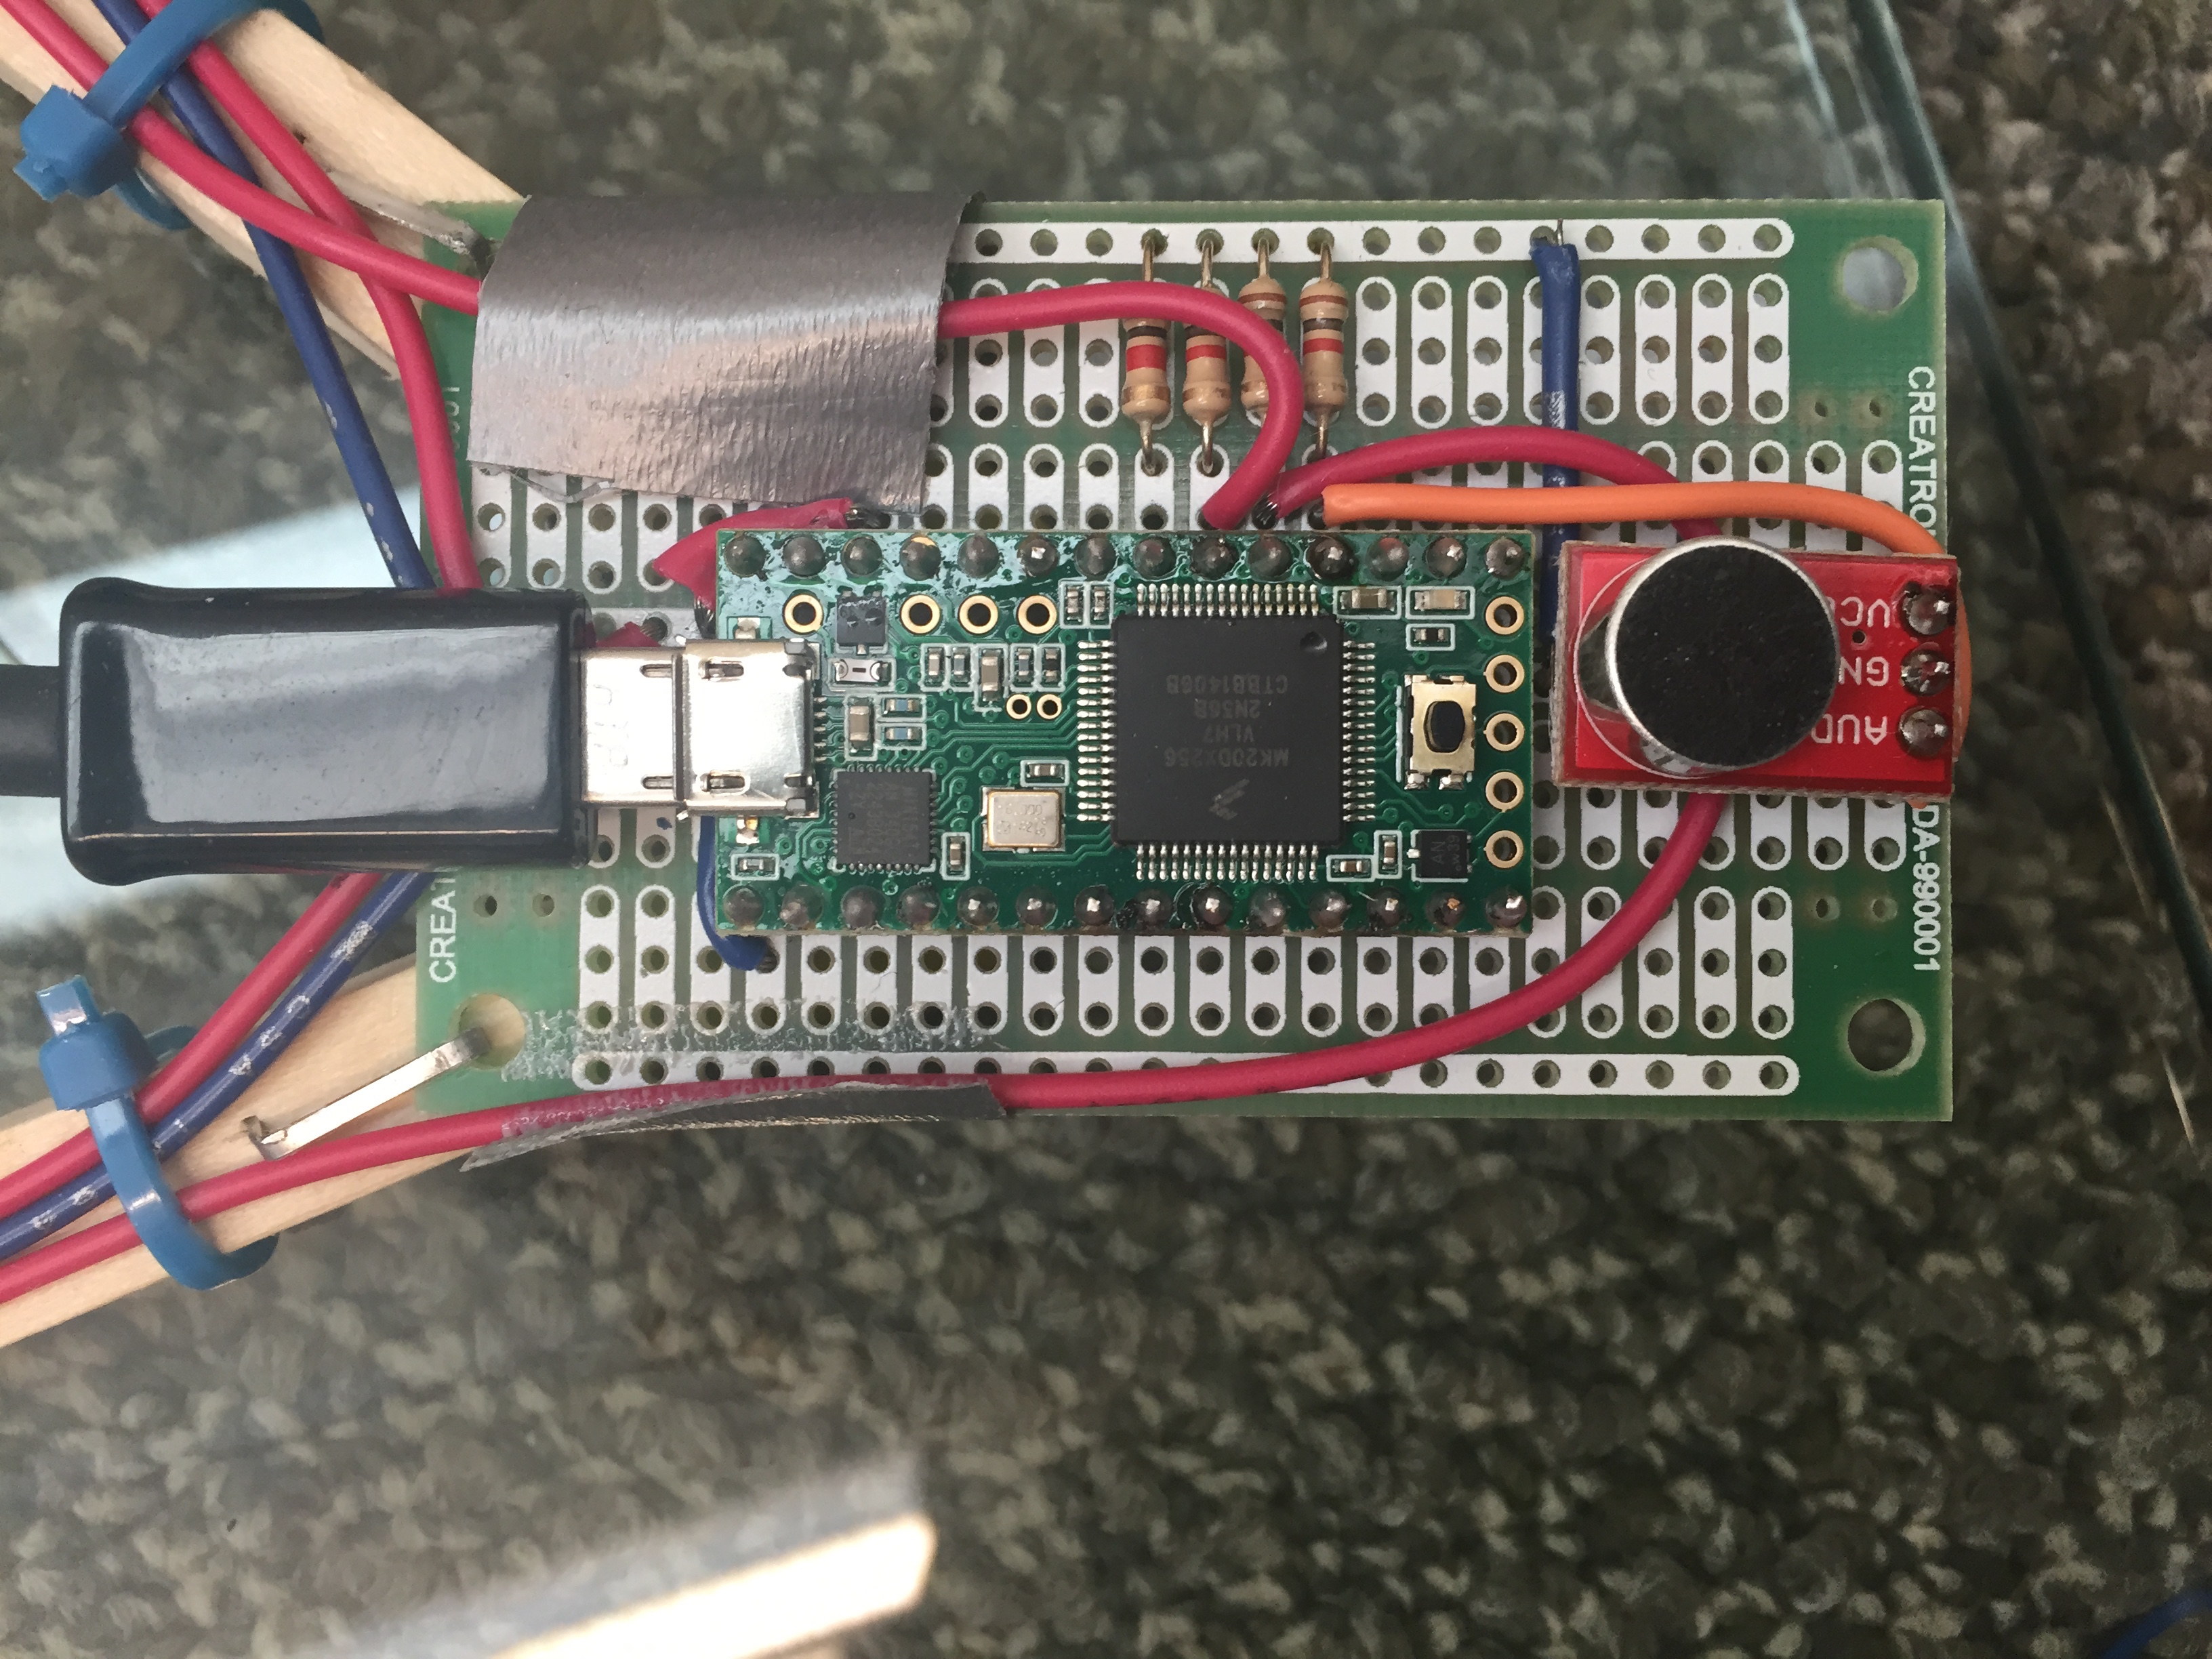
\includegraphics[width=\textwidth]{array_close.JPG}
    \caption{micro-controller}
  \end{subfigure}
  \begin{subfigure}[]{.48\textwidth}
    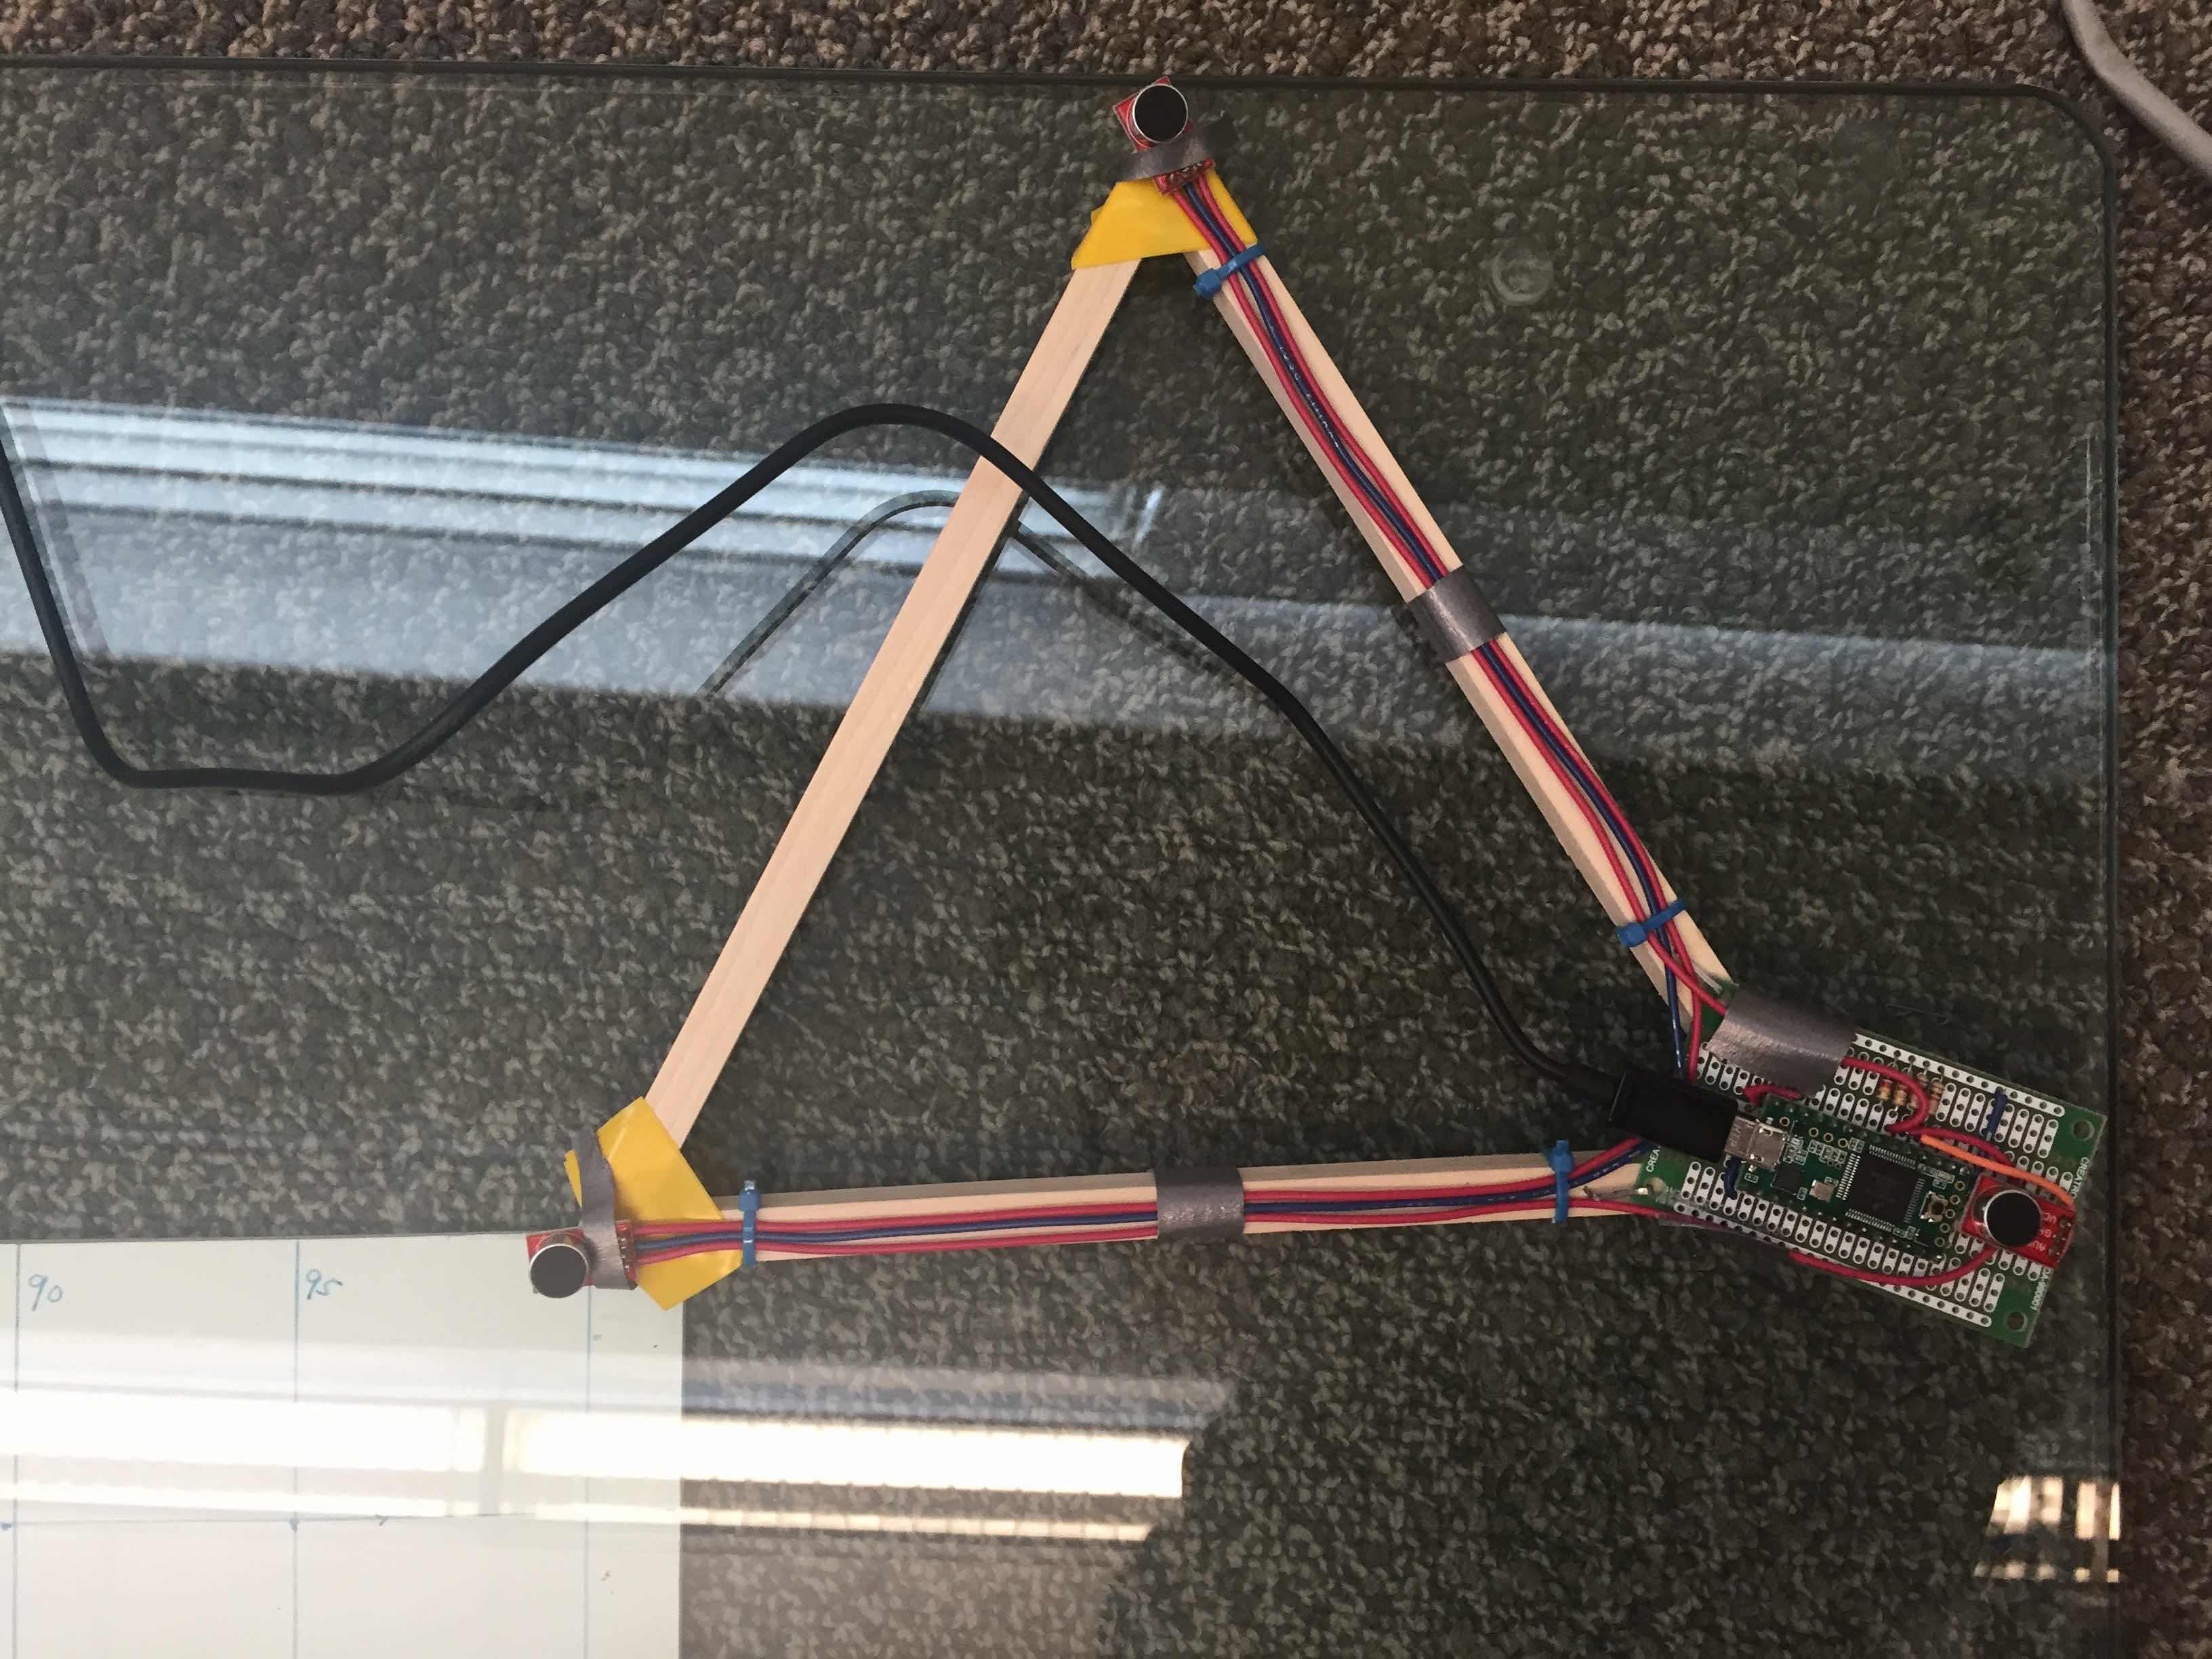
\includegraphics[width=\textwidth]{array.JPG}
    \caption{array}
  \end{subfigure}
  \begin{subfigure}[]{.48\textwidth}
    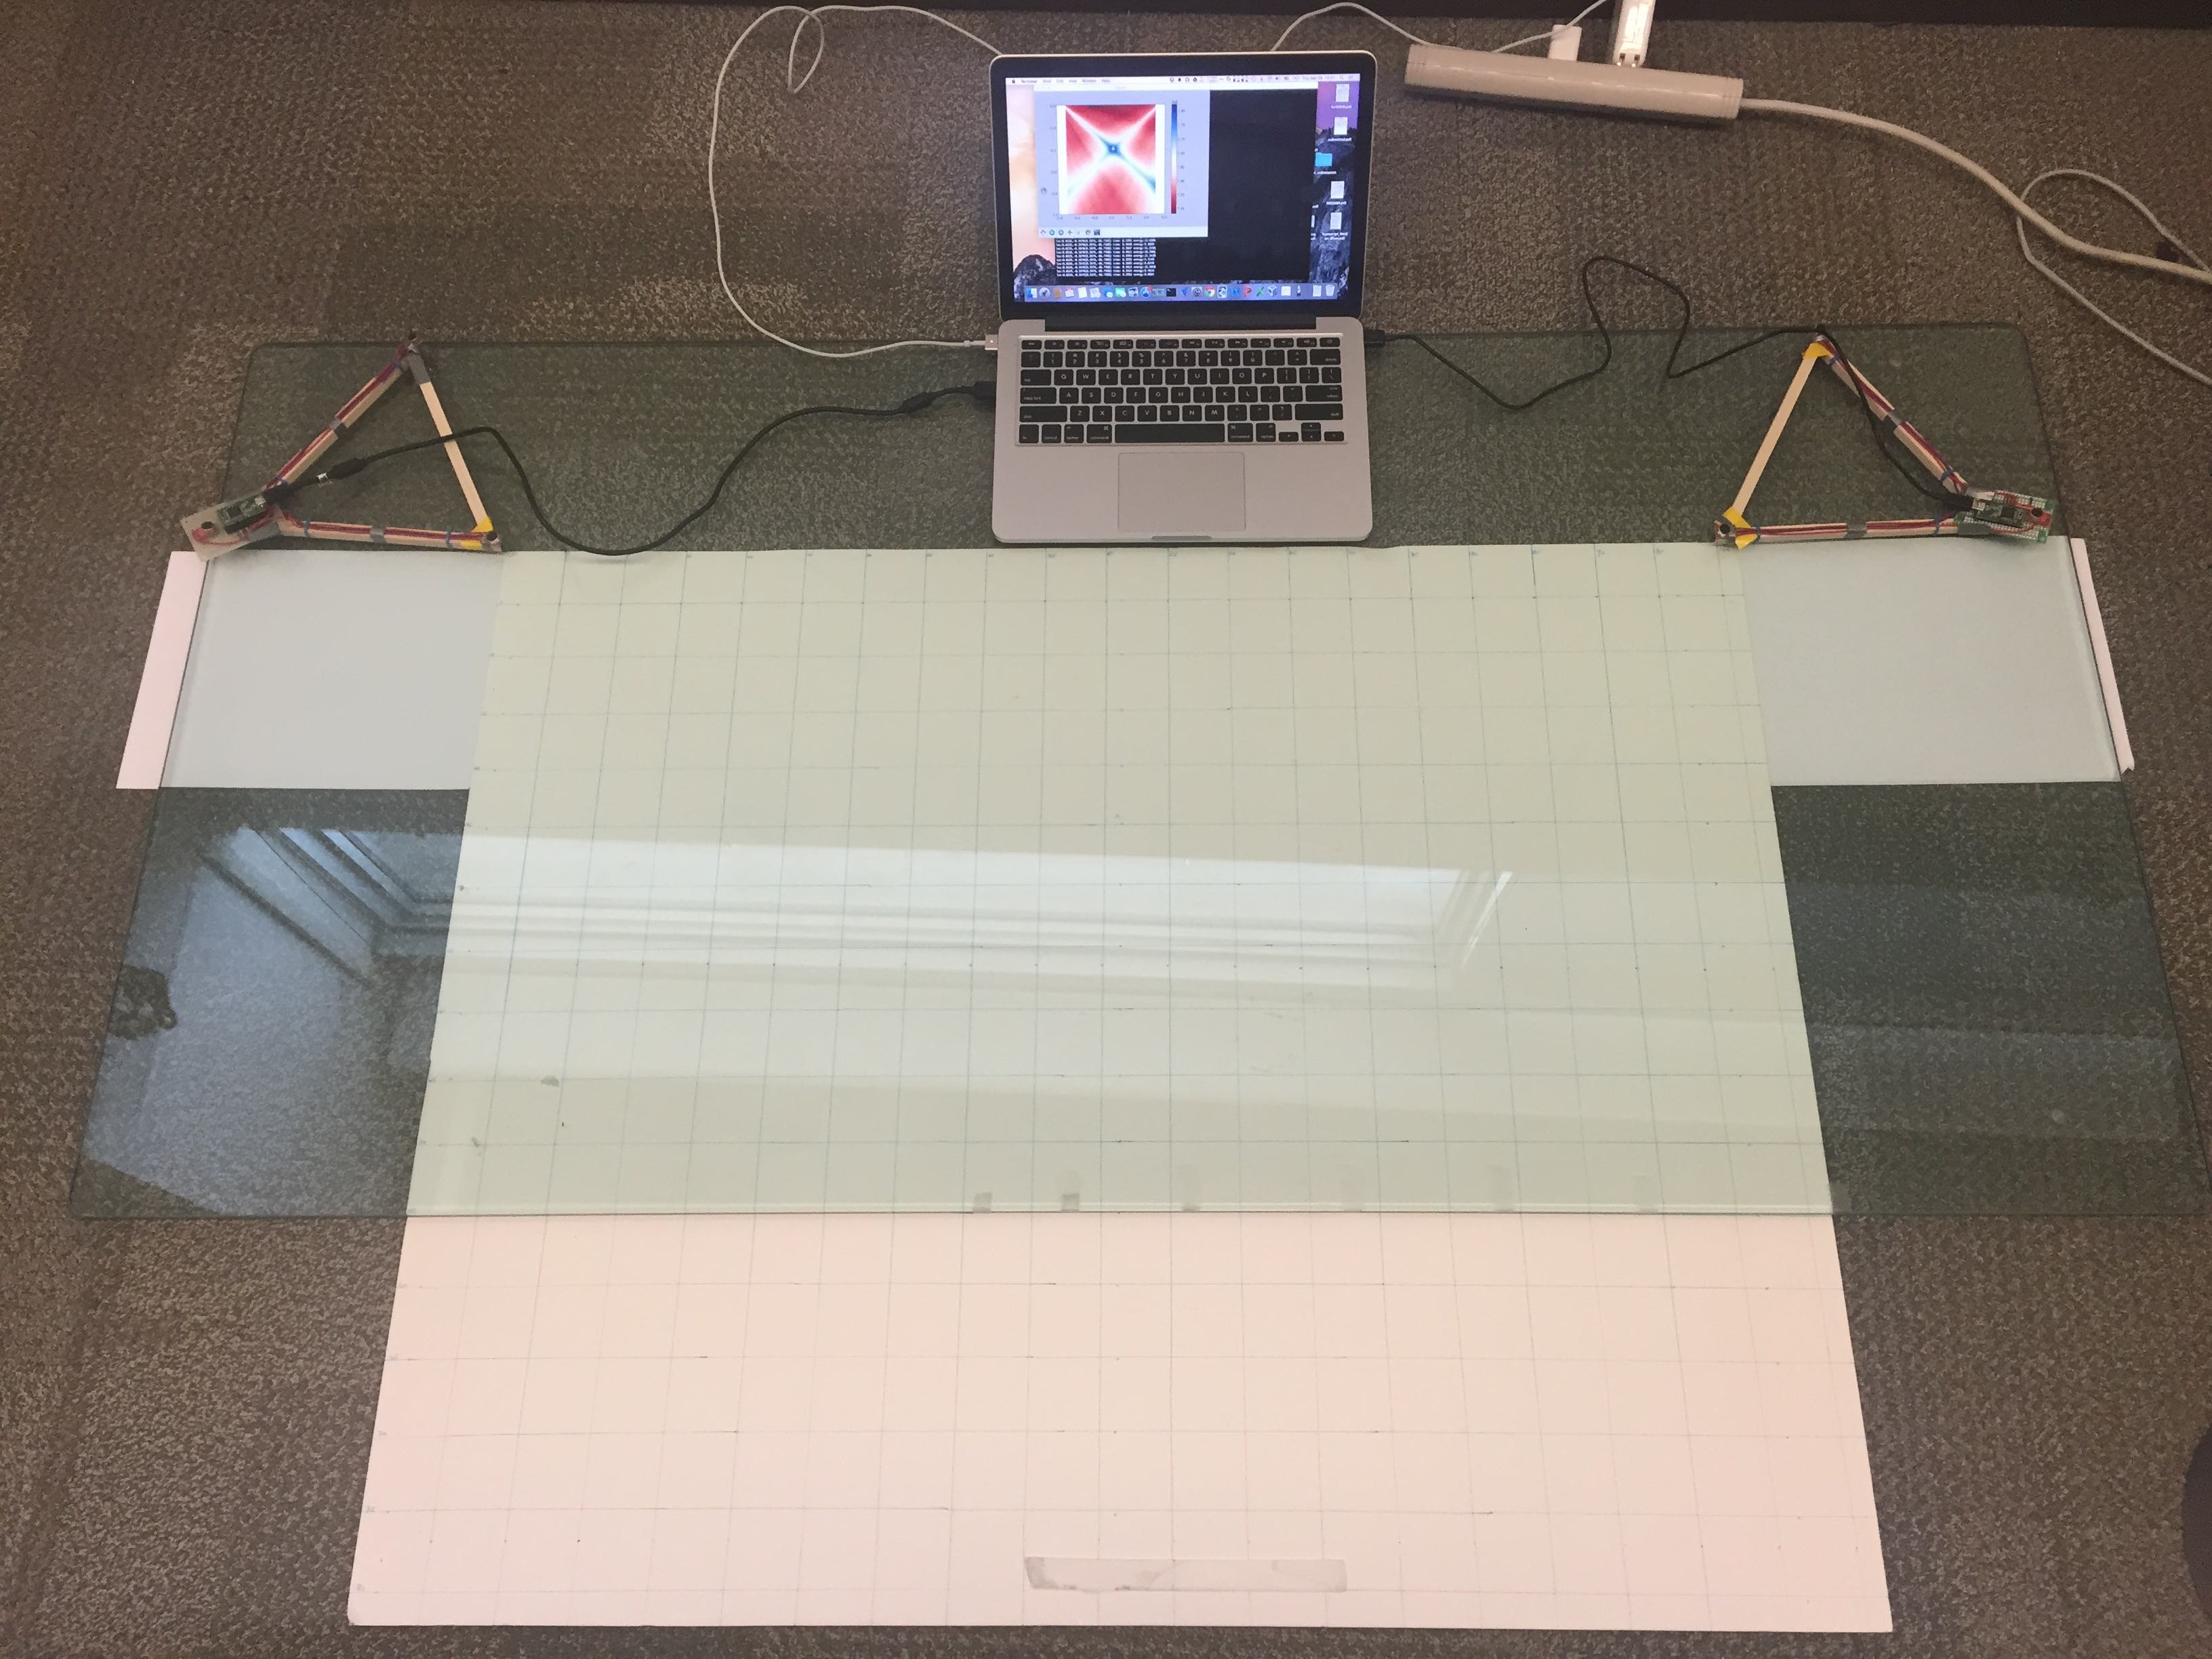
\includegraphics[width=\textwidth]{setup_2.JPG}
    \caption{two arrays}
  \end{subfigure}
  \caption{Localization system setup}
  \label{fig:setup_array}
\end{figure}

\subsection{Software}

On the software side, \emph{Python} is used as the main programming language since it has extensive libraries in both real time data handling and signal processing. \emph{ZeroMQ} is an inter process messaging queue that is used in our system to pass data across different modules. Our system is made up of two data acquisition modules (each is used to receive raw date from microphone array output) and one localization module (listens to both data acquisition modules and perform localization using the raw microphone data). Using ZeroMQ as connections to different modules adds flexibility to our system, as we can design applications such as the drawing application we have used in our system to interface only with the localization module and disregard how the microphone data is collected. Other localization applications can be easily integrated into our system by connecting them with the localization module. Furthermore, we have built a recording module that interfaces with the data acquisition modules for offline analysis and parameter tuning. 

To handle the uncertainty in TDOA estimation, instead of using point estimate that maximizes equation~\ref{eq:gcc}, we take the cross-correlation output(equation~\ref{eq:gcc2}) as a measure of the likelihood of different arrival time differences. Each index $i$ from the cross-correlation vector denotes the time delay across the two microphones receiving the acoustic signal, and the cross-correlation value $k$[i] at each index $i$ denotes the likelihood of the time delay being $i$. 

For each microphone array, we build a heatmap of likelihood for the region. The intensity at each point on the heatmap represents the likelihood of it being the source. To generate the likelihood heatmap for an microphone array, we apply the following algorithm. For each point ($x$,$y$) on the grid, the theoretical TDOA to each microphone pair can be precomputed using:
\[
 D_{m_1,m_2}(x,y) =  \frac{((x-x_1)^2 + (y-y_1)^2)^{0.5} - ((x-x_2)^2 + (y-y_2)^2)^{0.5}}{v}
\]
where ($x_1, y_1$) and ($x_2, y_2$) are the locations of the microphone pair and $v$ is the speed of sound. Then the heatmap can be generated by going through all the points on the grid and performing a lookup using equation~\ref{eq:gcc2}. With three microphones $m_1,m_2,$ and $m_3$, there are three microphone pairs: $m_1m_2,m_1m_3,$ and $m_2m_3$. The theoretical TDOA from each location $(x,y)$ to each microphone pair is precomputed and stored in $D_{m_1,m_2}(x,y)$, $D_{m_1,m_3}(x,y)$, and $D_{m_2,m_3}(x,y)$. Then the likelihood map $L(x,y)$ can be built by superposing the likelihood from each microphone pair:
\begin{eqnarray*}
L(x,y) &=& R_{m_1,m_2}(D_{m_1,m_2}(x,y)) + R_{m_1,m_3}(D_{m_1,m_3}(x,y)) \\
 & & +R_{m_2,m_3}(D_{m_2,m_3}(x,y)) 
\end{eqnarray*}
where $R_{m_1,m_2}(\tau)$,$R_{m_1,m_3}(\tau)$, and $R_{m_2,m_3}(\tau)$ denote GCC output from microphone pairs $m_1m_2,m_1m_3,$ and $m_2m_3$.

Likelihood maps from two arrays can be combined into the final likelihood map:
\begin{equation}\label{eq:combine_l}
L(x,y) = L_1(x,y) L_2(x,y)
\end{equation}
where $L_1(x,y)$ and $L_2(x,y)$ represent the likelihood map from array $1$ and array $2$.

\begin{figure}[h!]
  \centering
  \begin{subfigure}[]{.48\textwidth}
    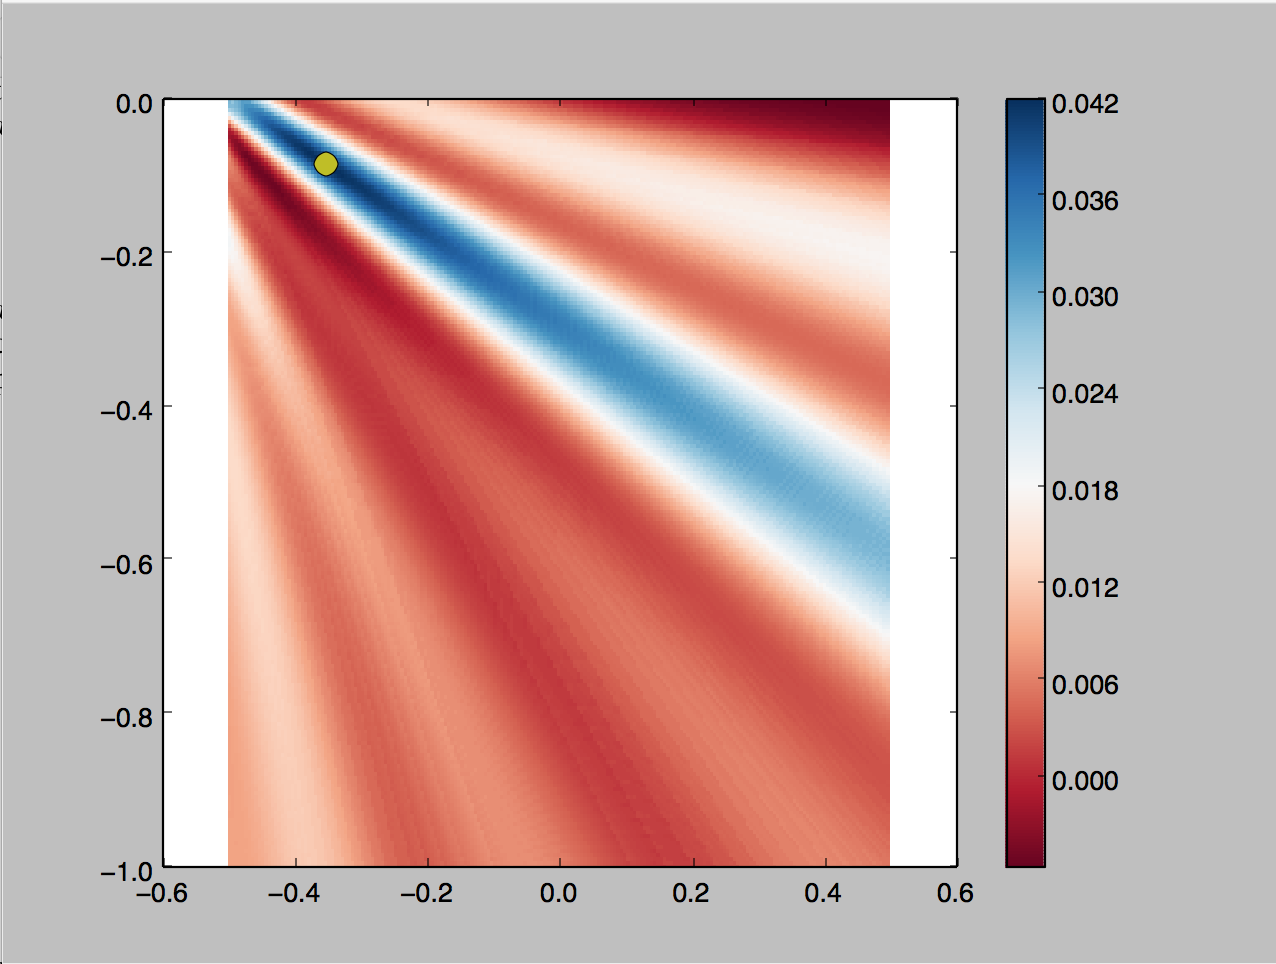
\includegraphics[width=\textwidth]{left.png}
    \caption{localization with only array 1}
    \label{fig:liklihood1}
  \end{subfigure}
  \begin{subfigure}[]{.48\textwidth}
    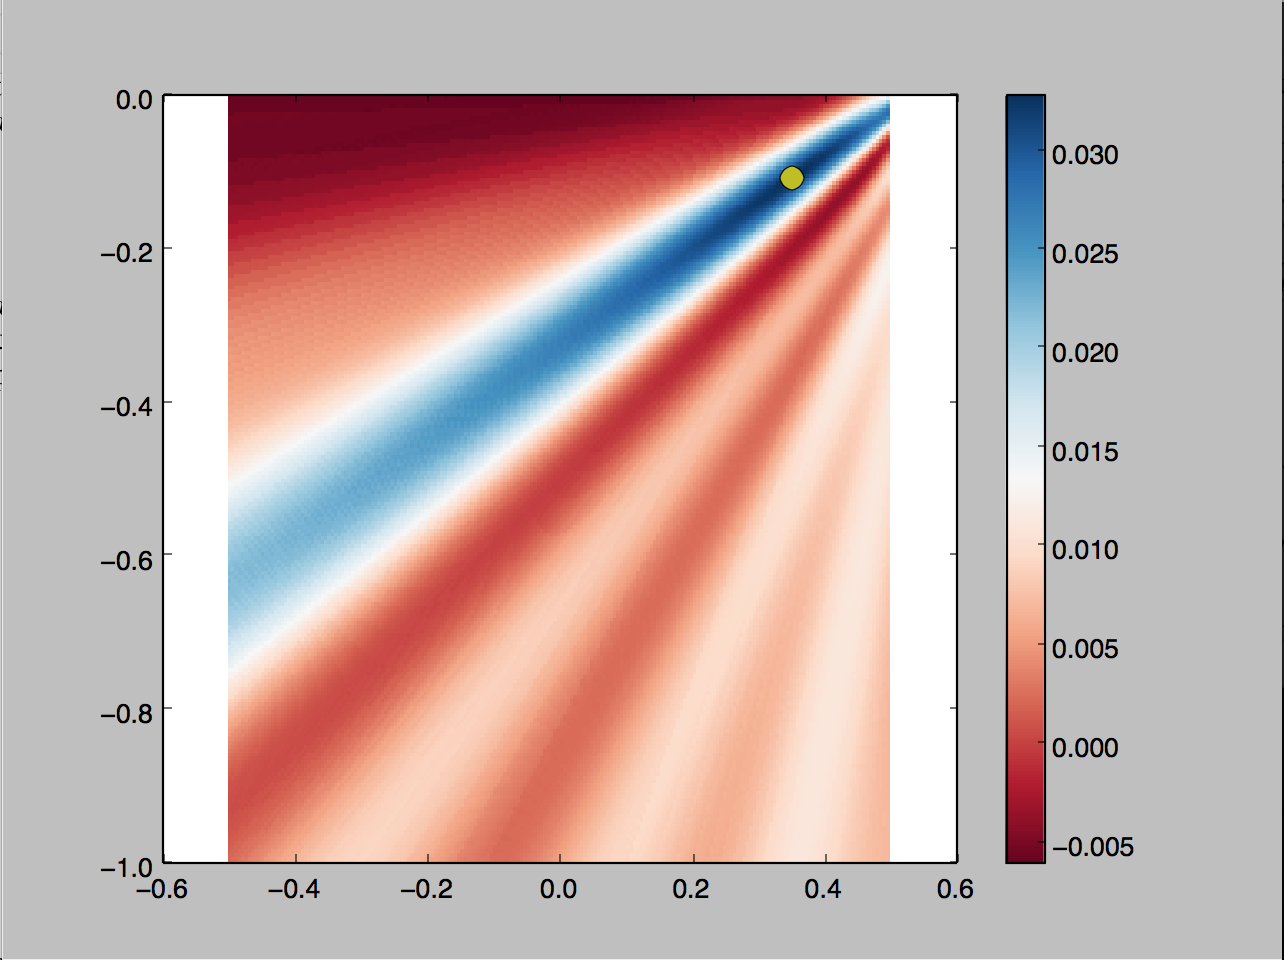
\includegraphics[width=\textwidth]{right.png}
    \caption{localization with only array 2}
    \label{fig:liklihood2}
  \end{subfigure}
  \begin{subfigure}[]{.48\textwidth}
    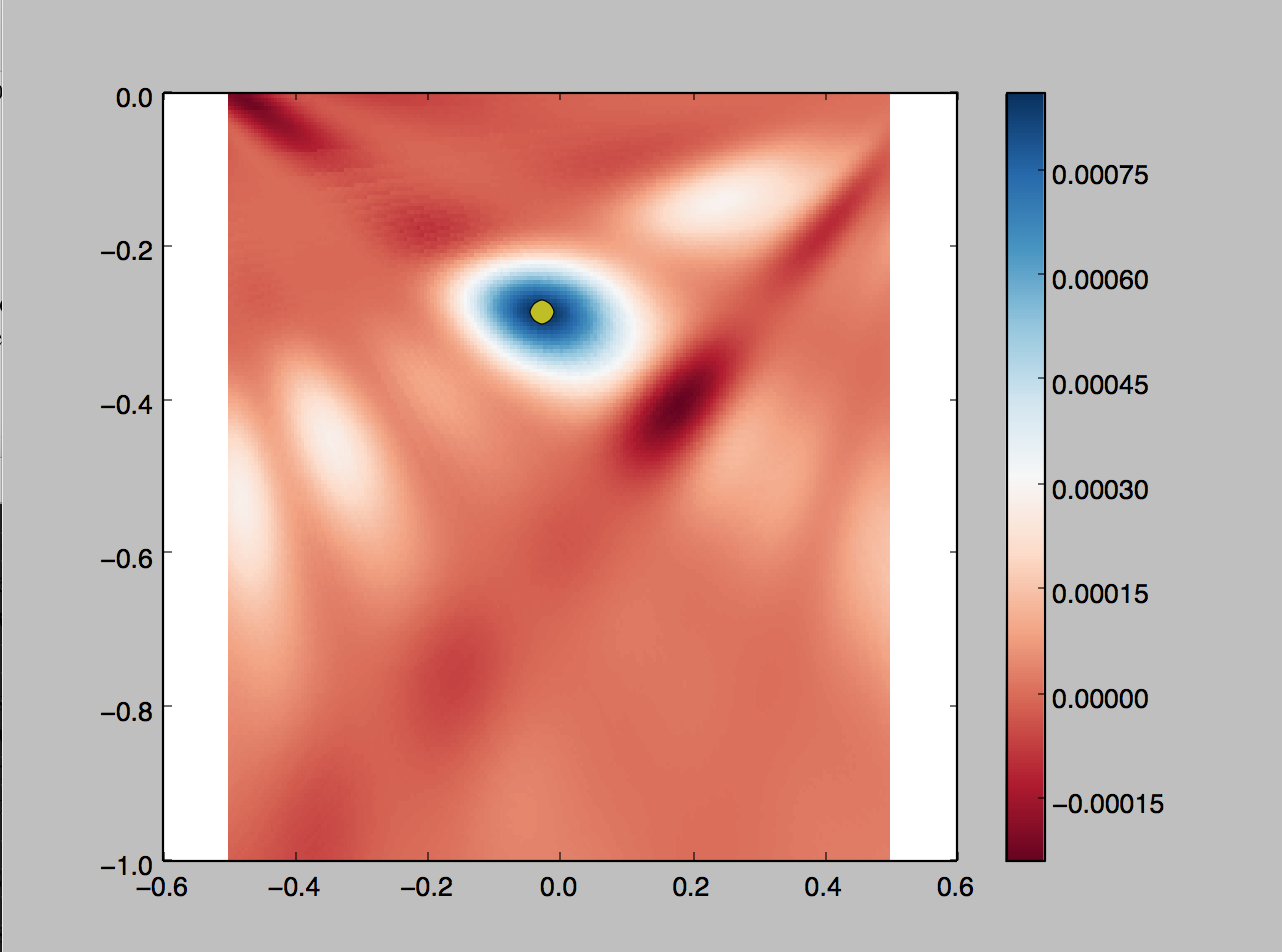
\includegraphics[width=\textwidth]{combined.png}
    \caption{localization with both arrays}
    \label{fig:liklihood3}
  \end{subfigure}
  \caption{Likelihood maps for localization. The source is placed at $(0.0,-0.3)$ m}
  \label{fig:liklihood}
\end{figure}

To see the effect of accuracy improvement using multiple arrays, fig~\ref{fig:liklihood} shows a real life localization where the source is placed at $(0$ cm$,-30$ cm$)$. The top two figures show the individual likelihood maps produced by single microphone arrays. We can see that the individual arrays can give accurate angle estimate, but have high uncertainty in distance estimate. The bottom figure shows the combined likelihood map according to equation~\ref{eq:combine_l}. The combined likelihood map demonstrated that by merging estimates from two arrays the system is able to perform more accurate localization. 


From a timing point of view, the micro-controller spends $12$ milliseconds on sampling the microphone data before sending it to a computer for processing. Sending the data through the USB port takes another $15$ milliseconds, and processing on the computer takes around $50$ milliseconds. Therefore, the total time lag between sound source and localization is around $80$ milliseconds.

\clearpage

\section{Setup}

We conducted two sets of experiments to evaluate the system's localization accuracy: one on point localization and the other on movement tracking. For the point localization experiment we looked into using different window size of audio signals and different prefiltering methods. The size of the window limits how far apart the microphone arrays can be. If the time delay from one microphone array to another exceeds the size of the window, the location of the source can never be estimated. A large window size gives a more complete acoustic signal which makes cross-correlation less prone to noise. However, the larger the window size the more time it takes to compute the cross-correlation. This is a trade off that we will address.  

For the movement tracking experiment, on top of the varying window size, we also looked into varying the movement speed of the audio source, applying different movement filters, and using different types of audio source. By applying an increasing movement speed of the audio source, we can test how fast the system can track an audible object moving in real time. We experimented with two types of music as our audio source for movement tracking, one with no low volume throughout, and the other with intermittent low or no volume. We want to test how the system performs when the audio source isn't continuously outputting sound. Furthermore, we applied different movement filters to help reduce noise and smooth out the path of the moving audio source.  

\subsection{Point localization}

\begin{figure}[h!]
  \centering
  \begin{subfigure}[]{.48\textwidth}
    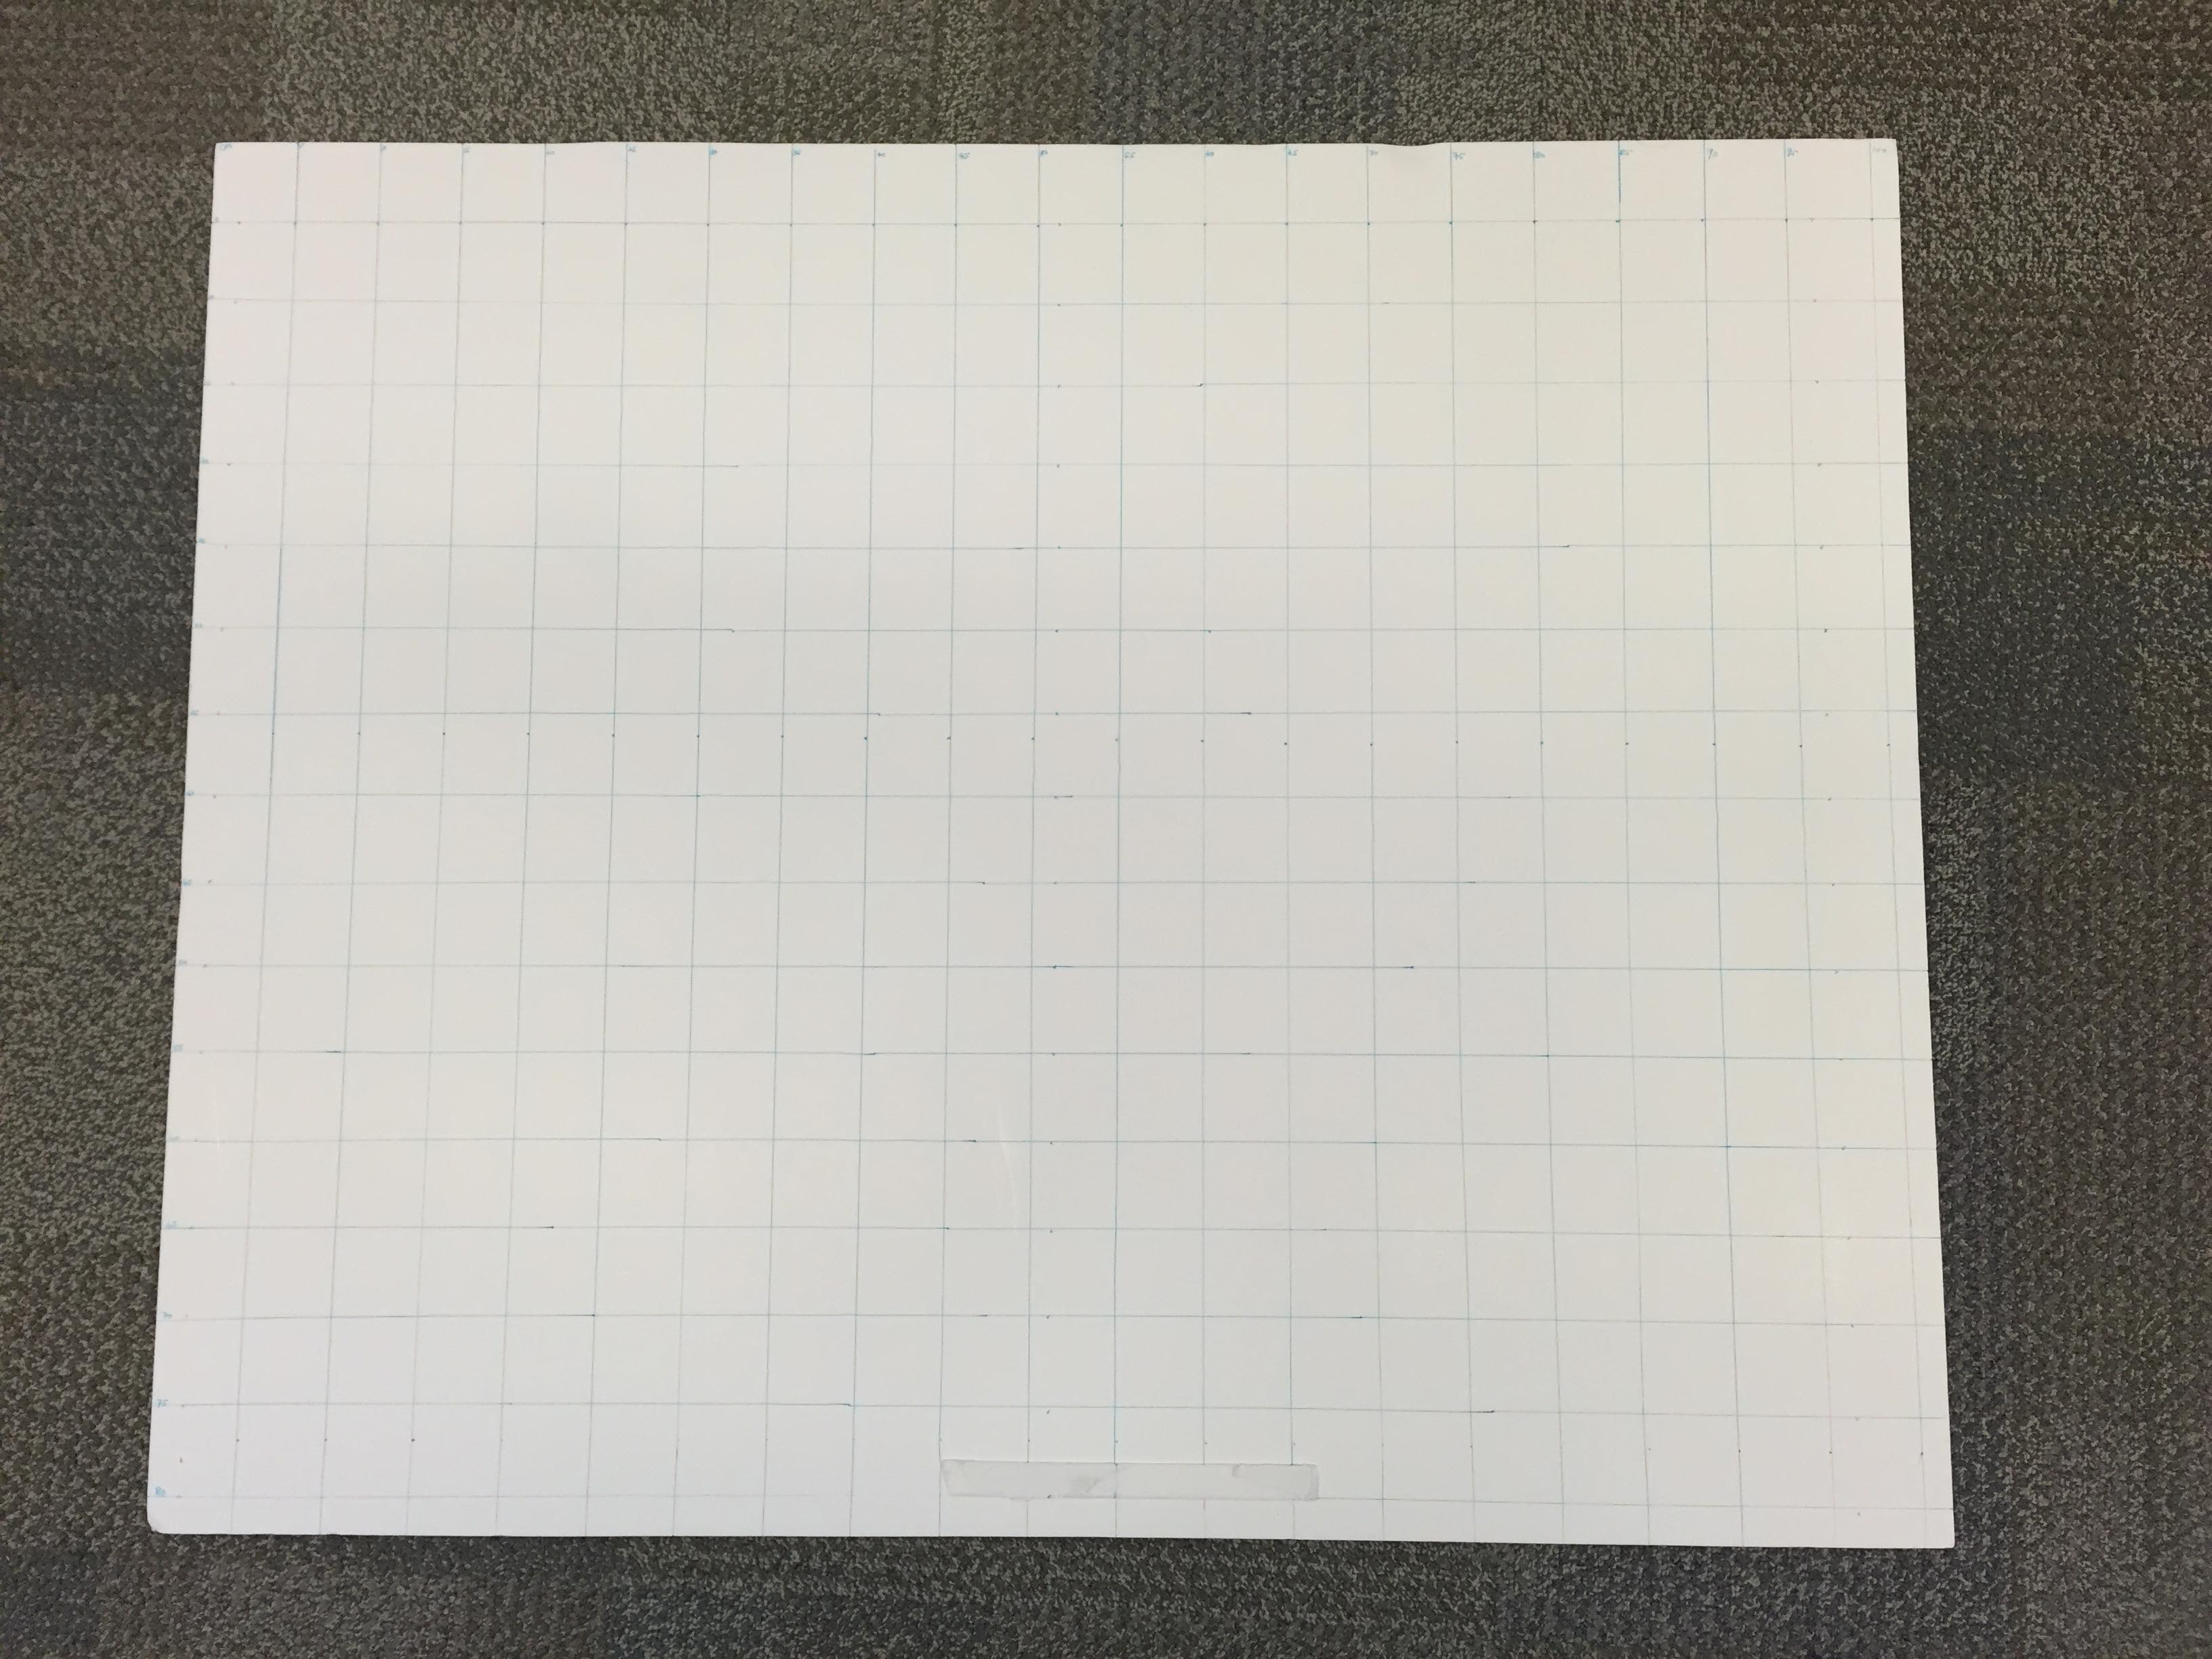
\includegraphics[width=\textwidth]{setup_1.JPG}
    \caption{1 meter by 1 meter grid}
  \end{subfigure}
  \begin{subfigure}[]{.48\textwidth}
    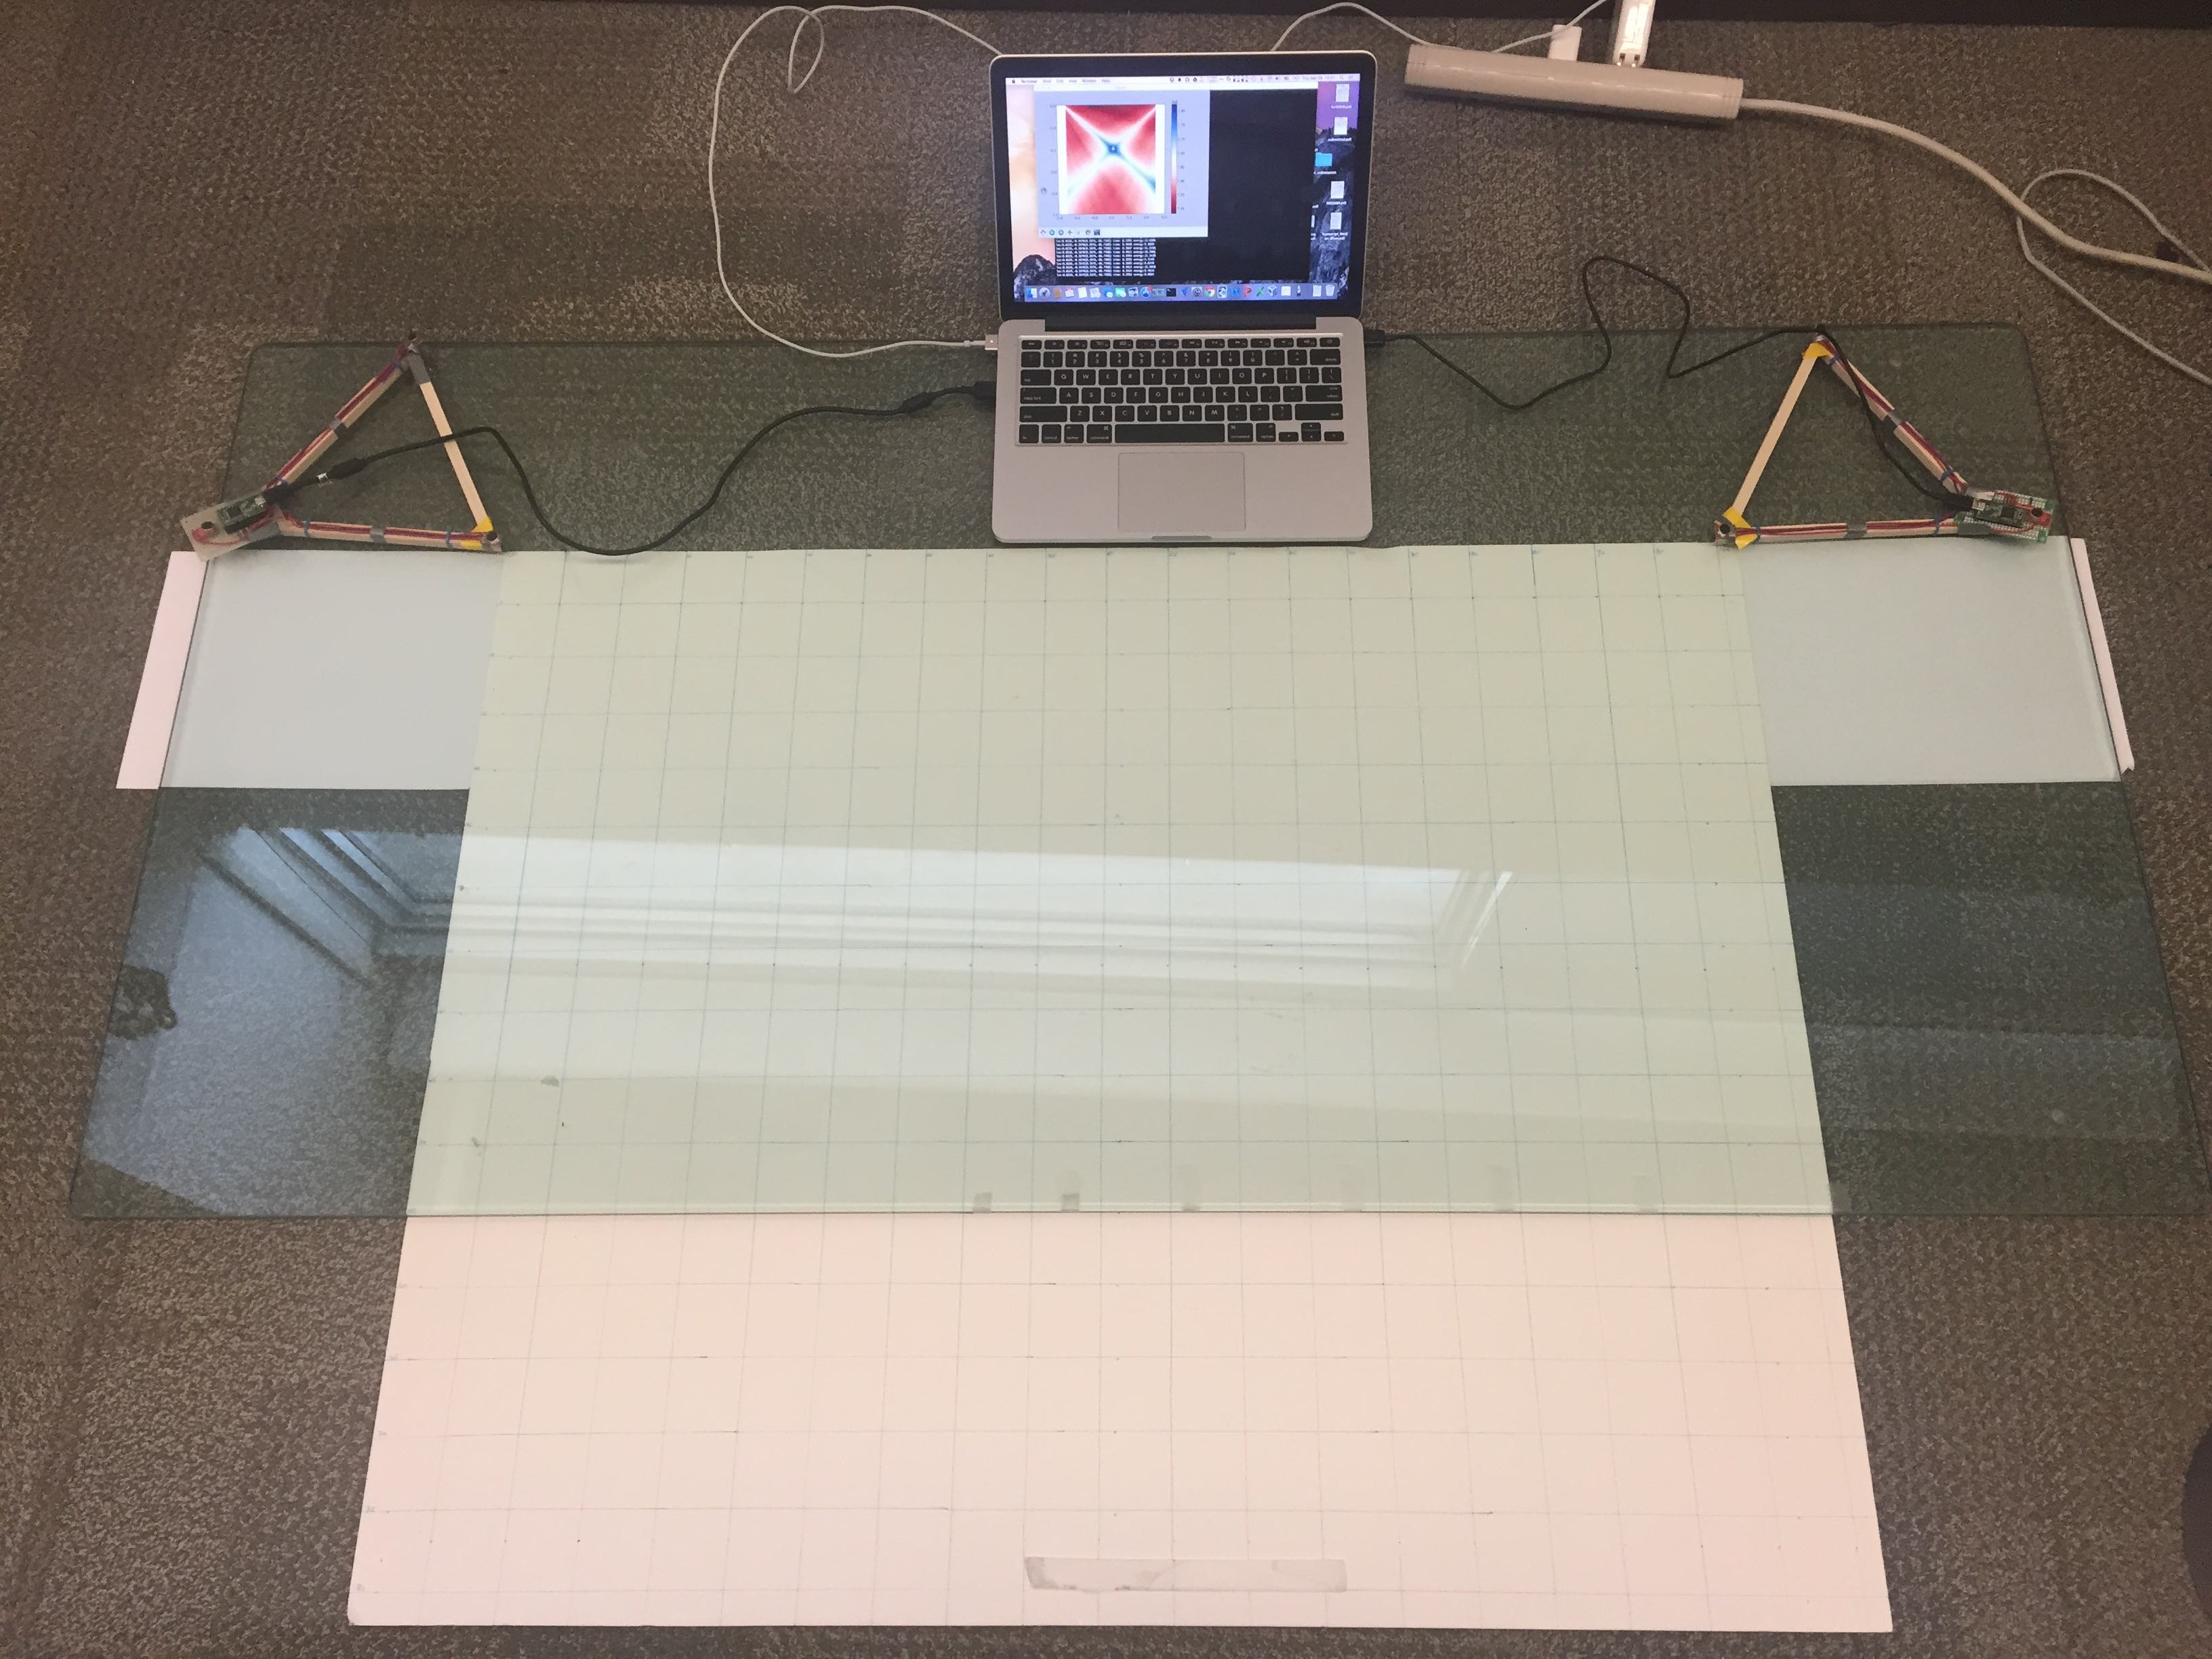
\includegraphics[width=\textwidth]{setup_2.JPG}
    \caption{array placement}
  \end{subfigure}
  \caption{Setup for point localization evaluation}
  \label{fig:setup_point}
\end{figure}

An one meter by one meter grid was set up where the arrays were placed at the top left and top right corners of the grid. Fig~\ref{fig:setup_point} shows a picture of the setup. A total of $32$ testing locations were chosen uniformly in this grid. Testing is done by placing the audio source at each grid location, and turning on the audio source with white noise. We reported the error as the average distance between our placement of the audio source and the location estimated from the arrays.

\subsection{Movement tracking}

\begin{figure}[h!]
  \centering
%  \begin{subfigure}[]{.2\textwidth}
%    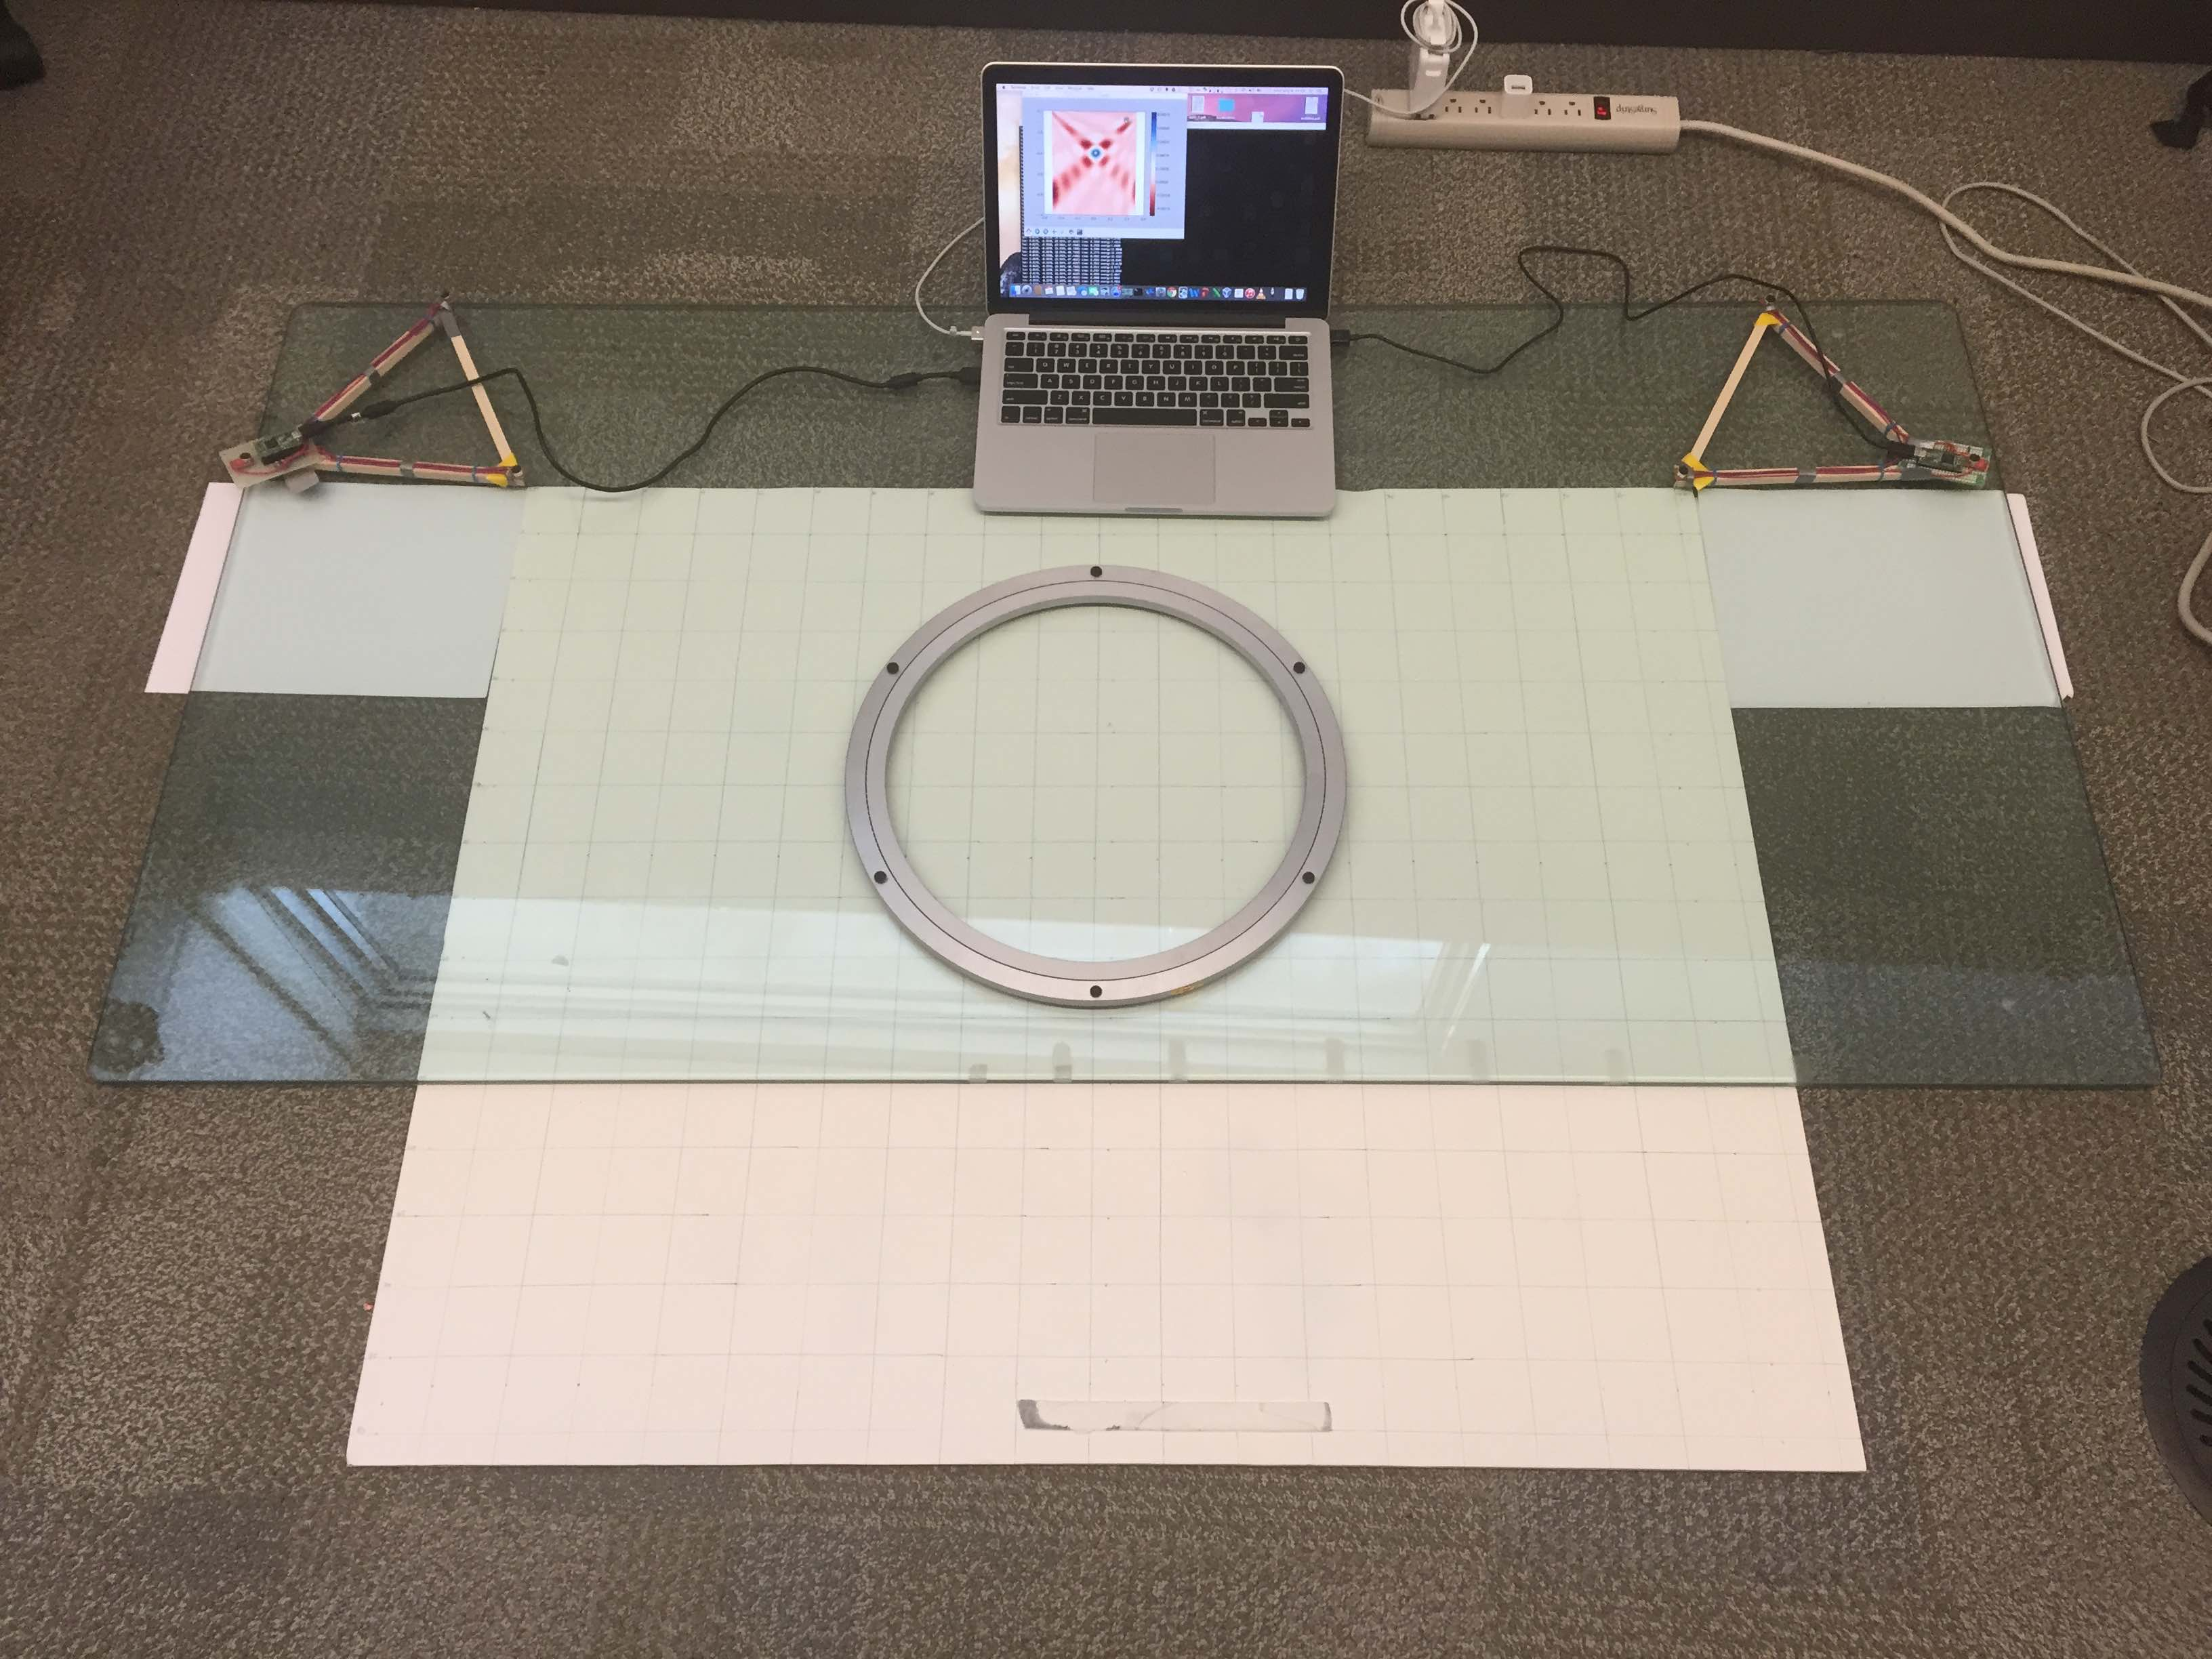
\includegraphics[width=\textwidth]{setup_ring.JPG}
%  \end{subfigure}
  \begin{subfigure}[]{1.0\textwidth}
    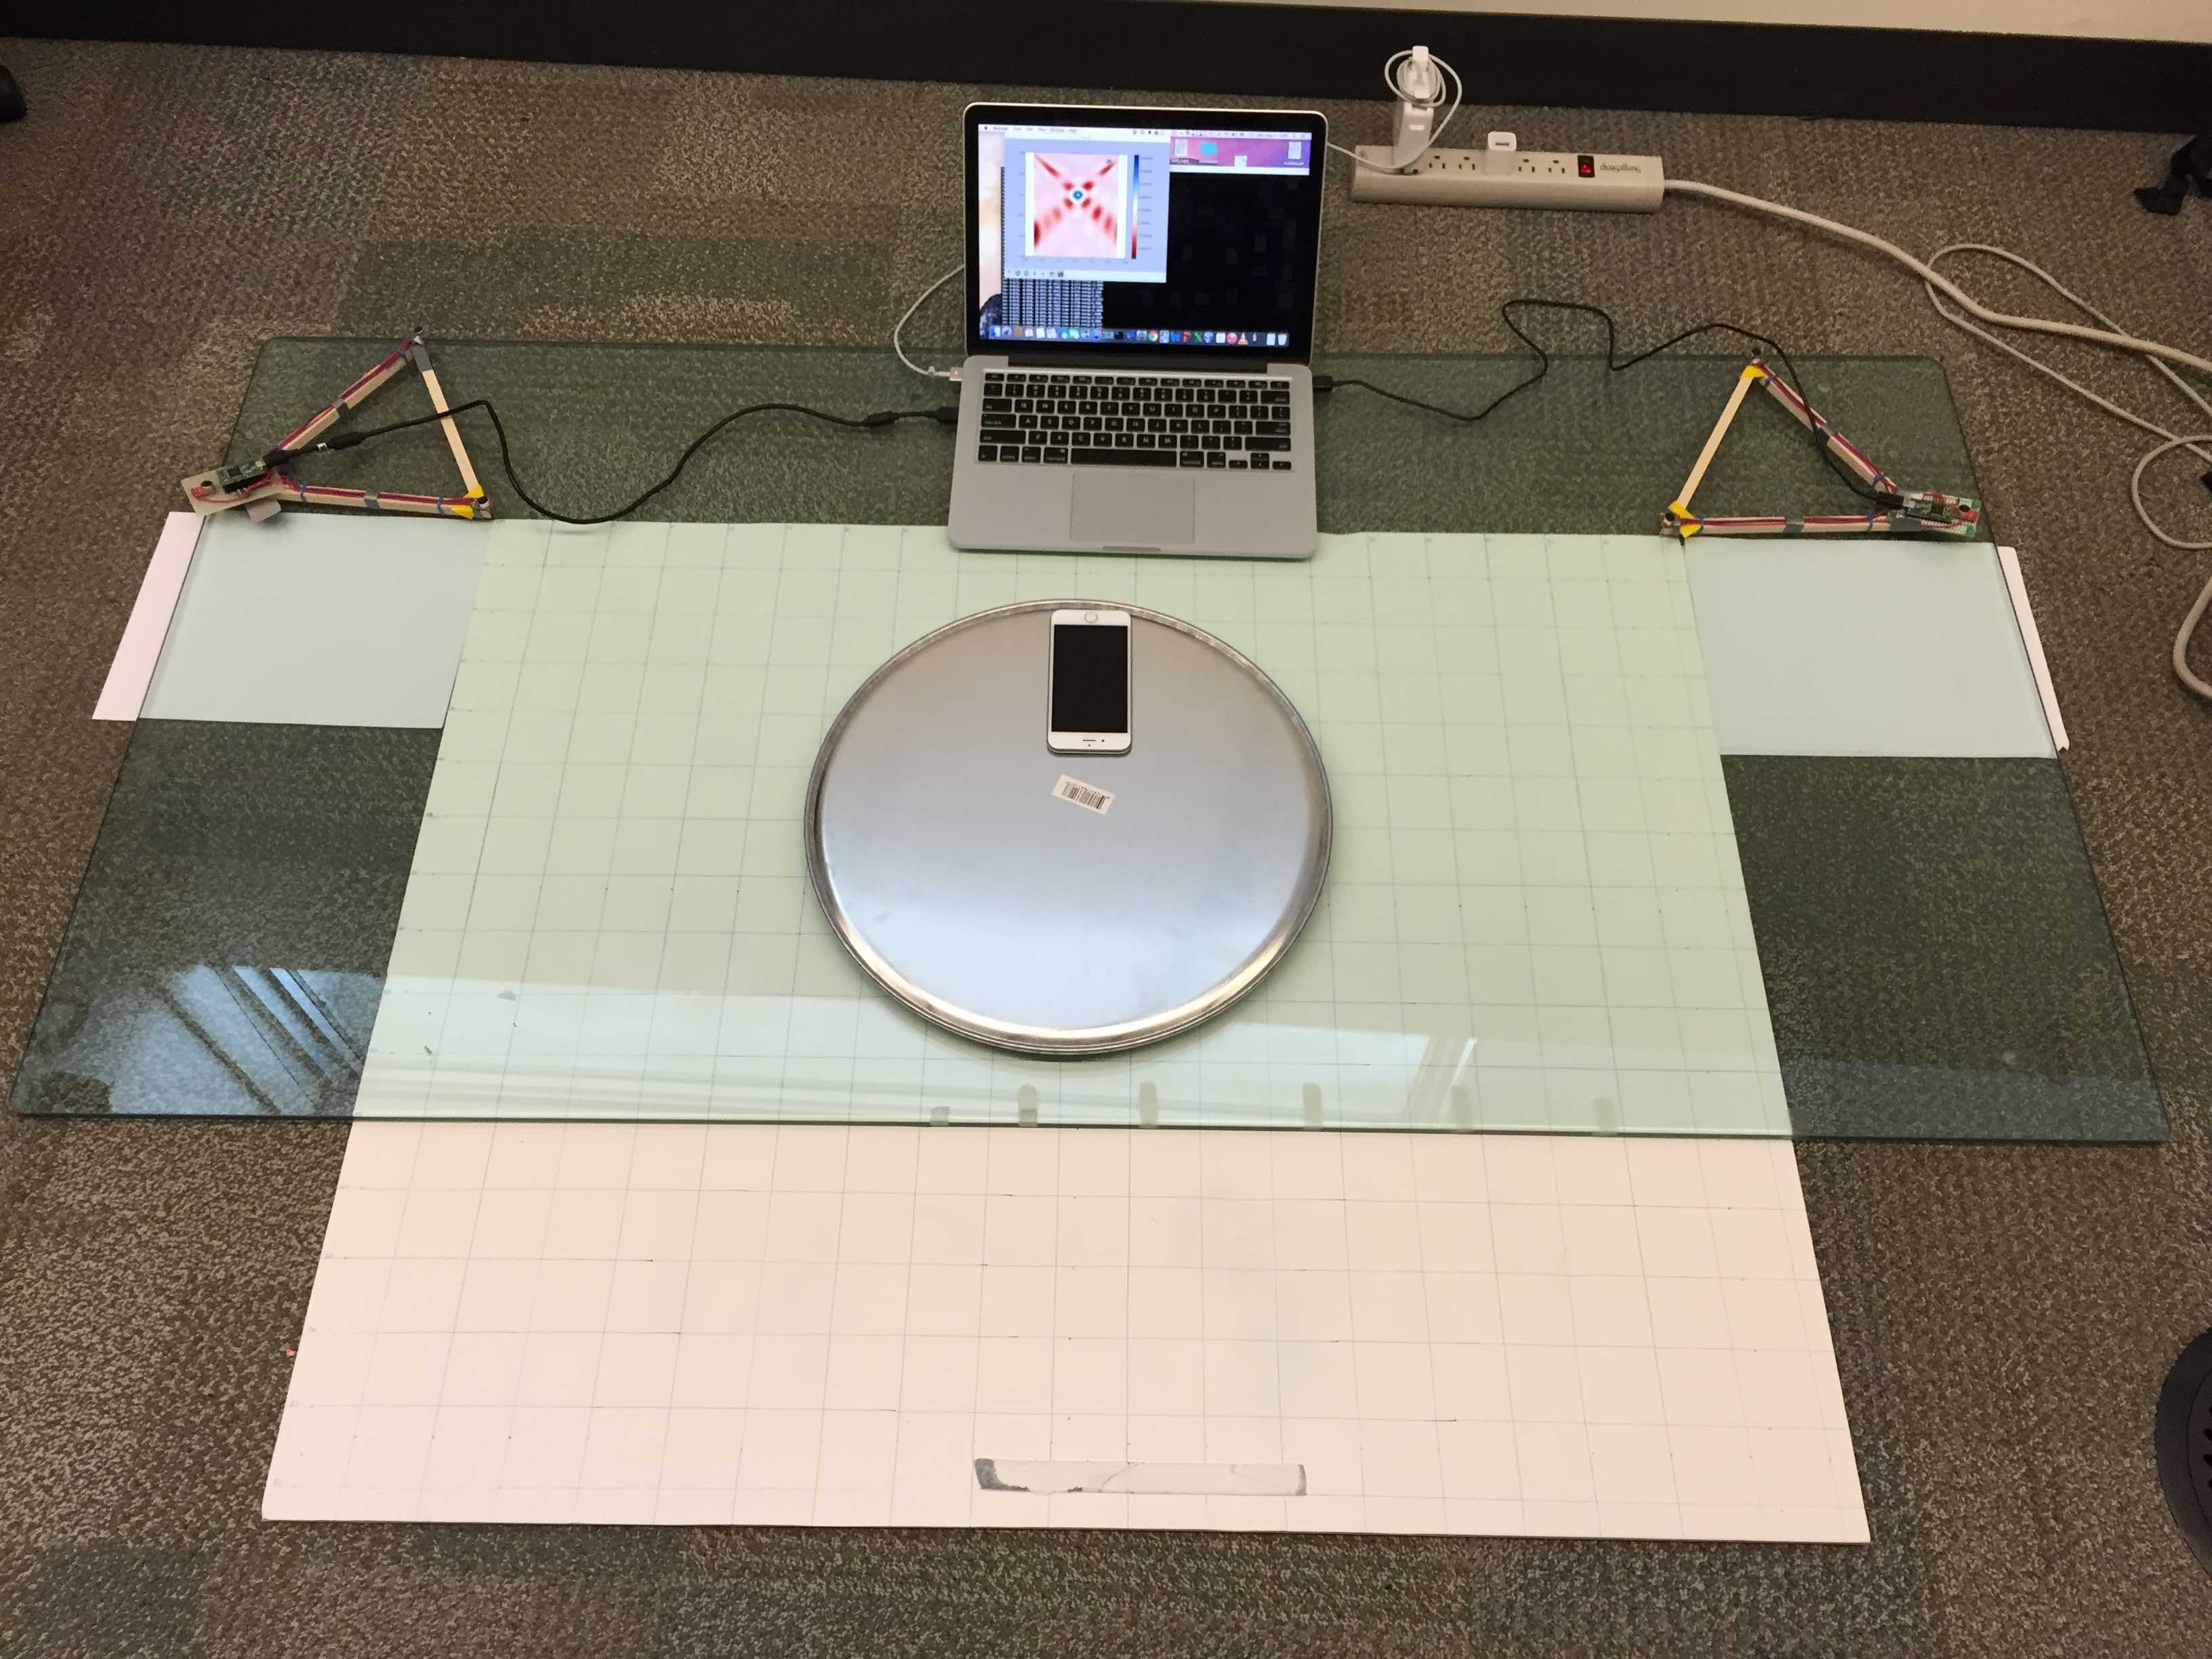
\includegraphics[width=\textwidth]{setup_rotating_disk.JPG}
  \end{subfigure}
  \caption{Setup for movement tracking evaluation}
  \label{fig:setup_circle}
\end{figure}


To test how well the system tracks movement, we mounted a rotating disk $40$ centimeters in diameter onto the grid at $(x=0$ cm$, y=-30$ cm$)$. Fig~\ref{fig:setup_circle} shows a picture of the setup. A sound source is placed on the edge of the rotating disk and the arrays track the sound source as it rotates in a circle. In this experiment we used GCC\_PHAT as the prefiltering for cross-correlation because in the point localization experiment we found out GCC\_PHAT gives the best result. In this experiment, we evaluated how accuracy changes with:
\begin{itemize}
\item window sizes 
\item audio sources
\item movement tracking filters
\item movement speeds
\end{itemize}

To test how localization accuracy varies with different window size of audio signal received, we conducted the experiment with audio signals with varying length from 1.02 ms to 12 ms.

To test how different sound sources impact localization quality, we conducted the experiments with three different sound sources:
\begin{description}%[\IEEEsetlabelwidth{long a label}\IEEEusemathlabelsep]

\item[White Noise] A recording of white noise. We expect GCC\_PHAT works best with white noise. The white noise is generated by sampling uniform randomly between $-1$ and $1$.

\item[Music A] A randomly picked music that has non-zero audio amplitude throughout the experiment period. \emph{Honest Eyes} by \emph{Black Tide} was the music used.

\item[Music B] A randomly picked music with intermittent low amplitude sections. \emph{Canon} was the music used.

\end{description} 

To test how the movement speed of sound source affects localization quality, each experiment was conducted at two different speeds:

\begin{description}
\item[Normal] An angular speed of $0.5$ rad/s was maintained, which translates to a linear speed of $10$ cm/s.
\item[Fast] An angular speed of $1.0$ rad/s was maintained, which translates to a linear speed of $20$ cm/s.
\end{description}

For each experiment conducted, two different movement filters were evaluated:
\begin{description}%[\IEEEsetlabelwidth{Very long label}\IEEEusemathlabelsep]
\item[Averaging filter] localization for past $0.5$ seconds were averaged and outputted as current estimate.
\item[Kalman filter] A 2nd order Kalman filter was used.
\end{description}

In the movement tracking experiments described above, we know the ground truth location of the circle, but not the exact location of the audio source at each moment during the movement. Therefore, the error is reported as the distance between the localized point to its closest point on the ground truth circle.
\clearpage

\section{Results}
\subsection{Point localization}
\begin{figure}[h!]
\centering
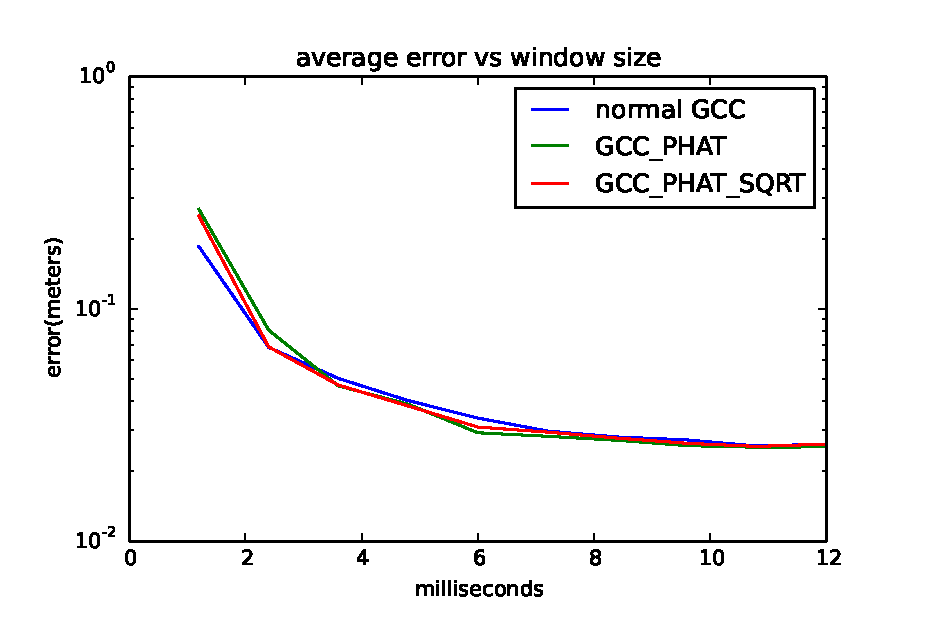
\includegraphics[width=1.0\textwidth]{average_error_window_size.eps}
\caption{Localization error versus window size}
\label{fig:accuracy_vs_window}
\end{figure}
To test how accuracy varies with window size, the algorithm is fed with microphone data of different lengths, and the result is shown in fig~\ref{fig:accuracy_vs_window}. The error decreases as window size increases and plateaus after the window size exceeds around $10$ millisecond. The lowest error achieved is $2.53$ centimeters, which occurred when the window size is set to 12 millisecond and when GCC\_PHAT is used for TDOA estimation. The performance differences among GCC, GCC\_PHAT and GCC\_PHAT\_SQRT is small.

\begin{figure}[h!]
\centering
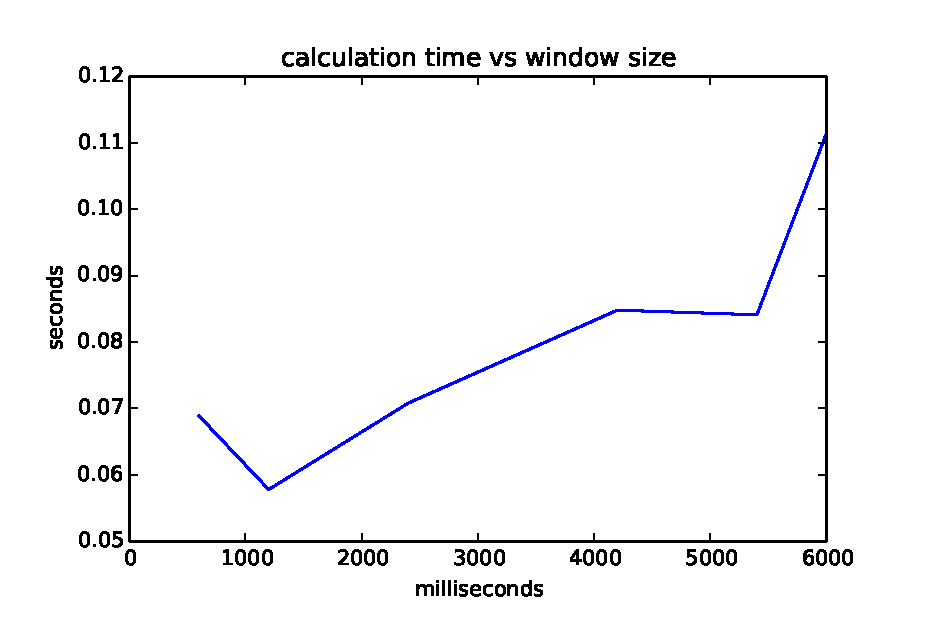
\includegraphics[width=1.0\textwidth]{calculation_time.eps}
\caption{Computation time versus window size}
\label{fig:speed_vs_window}
\end{figure}
As was mentioned before, although accuracy improves with the window size, computation time also increases with it. The part of calculation that depends on the window size is using cross correlation for TDOA estimation. Cross correlation can be calculated with Fast Fourier Transform (FFT) and the runtime is of order $O(N\log N)$. We measured how the computation time varied with window size and Figure~\ref{fig:speed_vs_window} shows the result. The runtime increases approximately linearly in the window size region of interest.

\begin{figure}[h!]
\centering
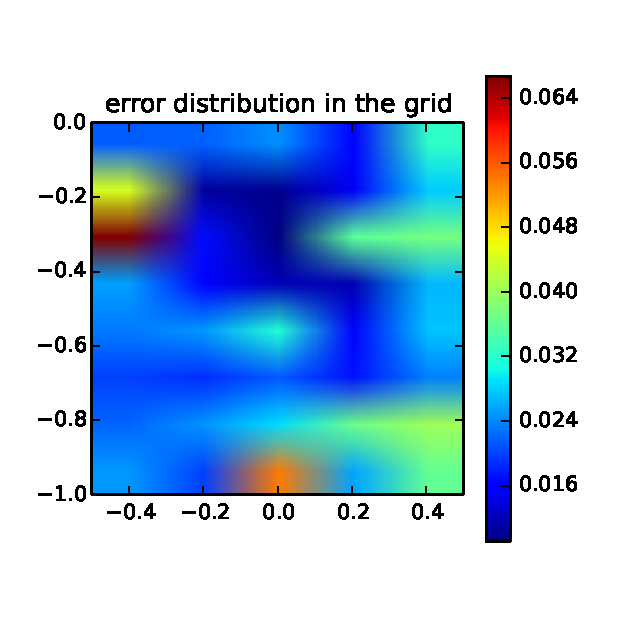
\includegraphics[width=1.0\textwidth]{error_distribution.eps}
\caption{error distribution in the grid. Arrays are placed at $(-0.5$ m$, 0$ m$)$ and $(0.5$ m$, 0$ m$)$}
\label{fig:error_distribution}
\end{figure}
We also calculated the localization error for each tested point in the grid. Figure~\ref{fig:error_distribution} shows the error distribution inside the grid. The error is below $3$ cm for most areas inside the grid. There is one error spike in the mid-left region and we contribute this to audio source misplacement because the error is fairly low and consistent around that spike.

\begin{figure}[h!]
\centering
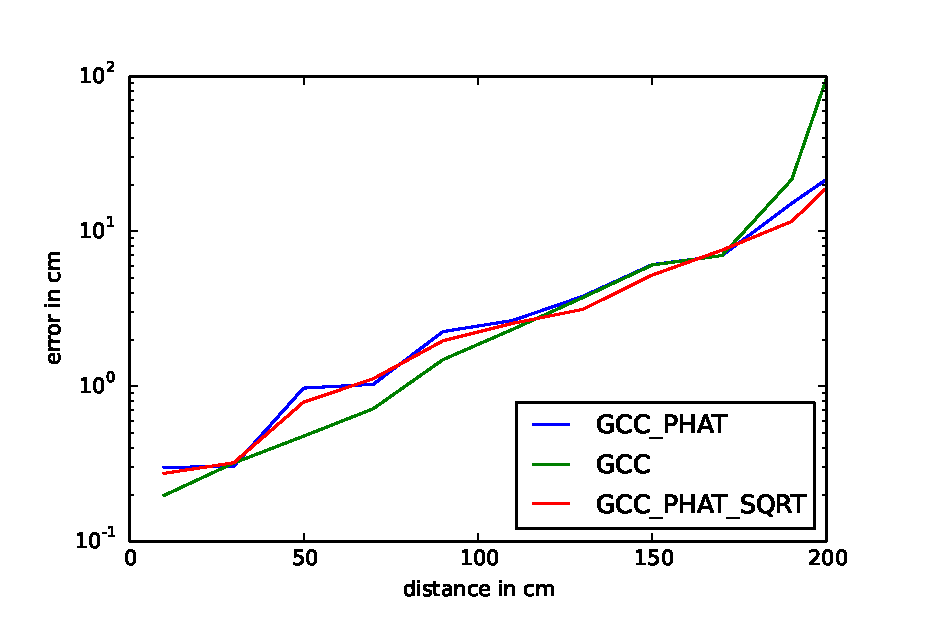
\includegraphics[width=1.0\textwidth]{error_along_y_axis.eps}
\caption{Localization error as the distance between the source and the microphone arrays increases. The source is placed on the $y$ axis.}
\label{fig:error_along_y}
\end{figure}
To test the limit of the system and to evaluate the accuracy when the source moves outside of the one meter by one meter region, we measured the localization error by placing the source at $10$ locations along $y$ axis ranging from $(0$ cm$, -10$ cm$)$ to $(0$ cm$, -200$ cm$)$. The result is presented in fig~\ref{fig:error_along_y}. The localization error is within $3$ cm when the source is within $100$ cm from the arrays. The error increases to about $5$ cm when the source distance increases to $150$ cm and the error exceeds $10$ cm after the source distance reaches $200$ cm.

\clearpage
\subsection{Movement tracking}
\begin{figure*}[h!]
\centering
  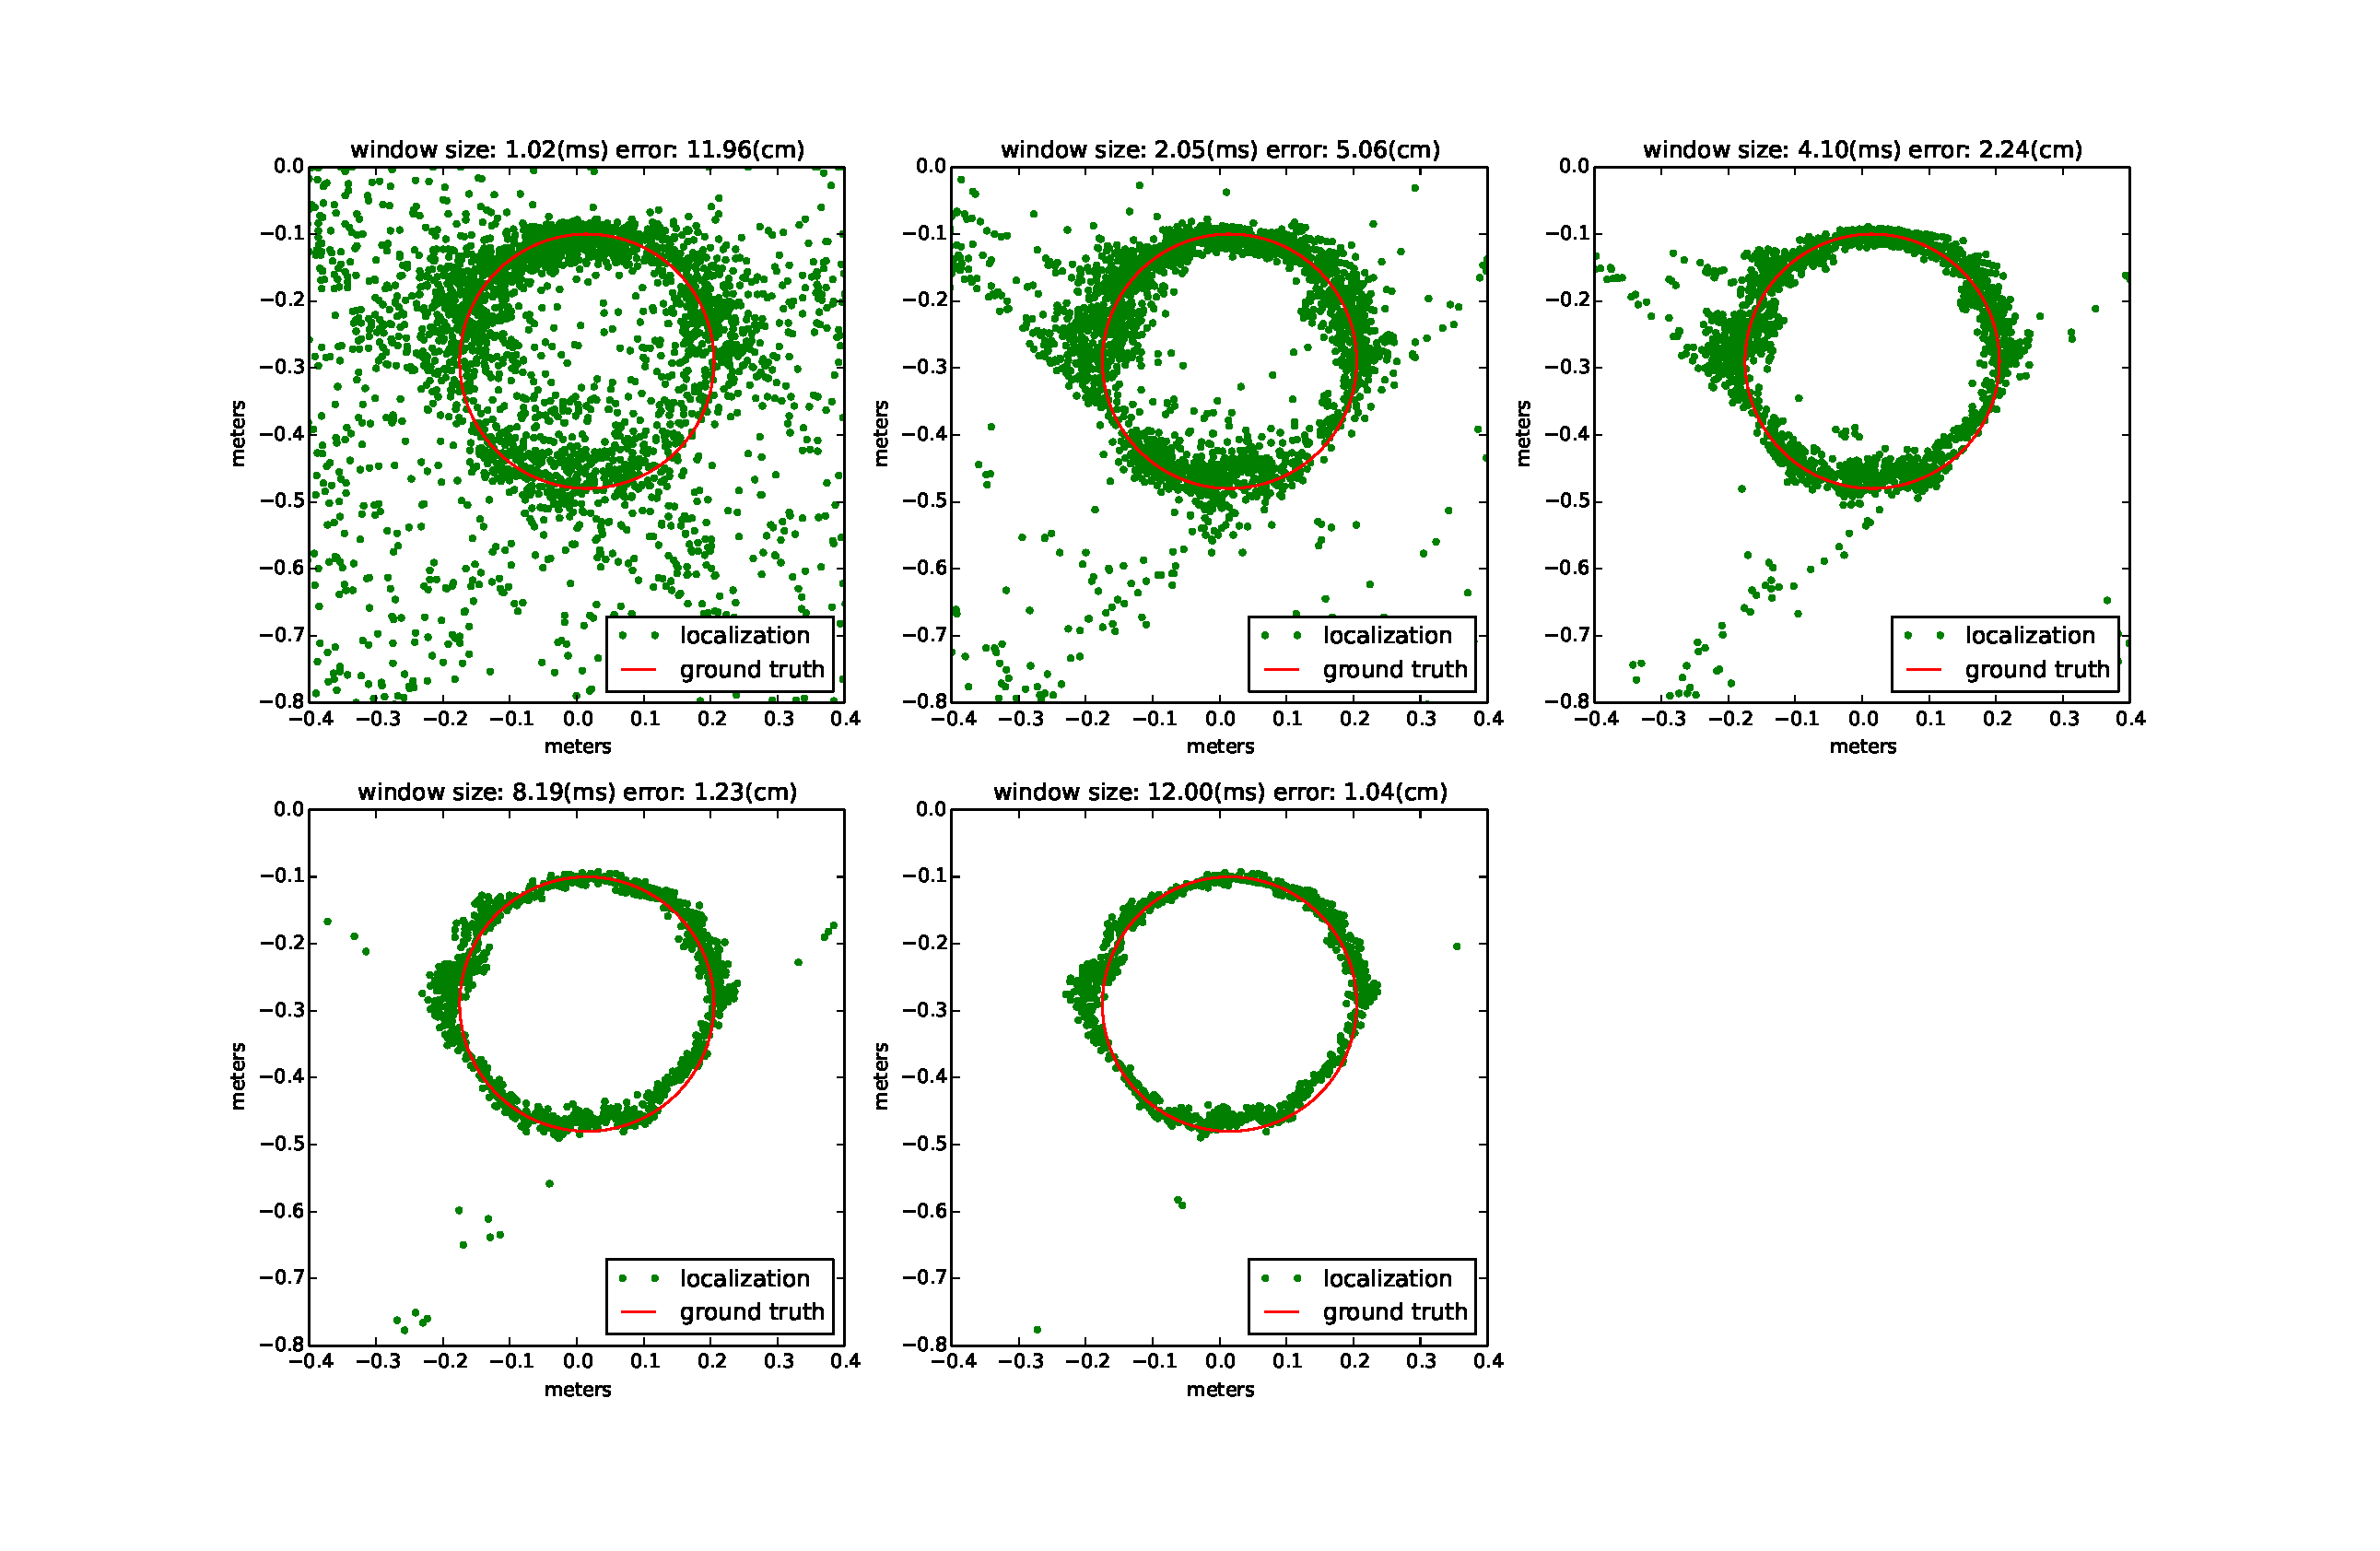
\includegraphics[width=\textwidth]{trace_window_size_movement.eps}
\caption{Localization quality versus window size}\label{fig:wn}
\label{fig:trace_win_circle}
\end{figure*}

\begin{figure}[h!]
\centering
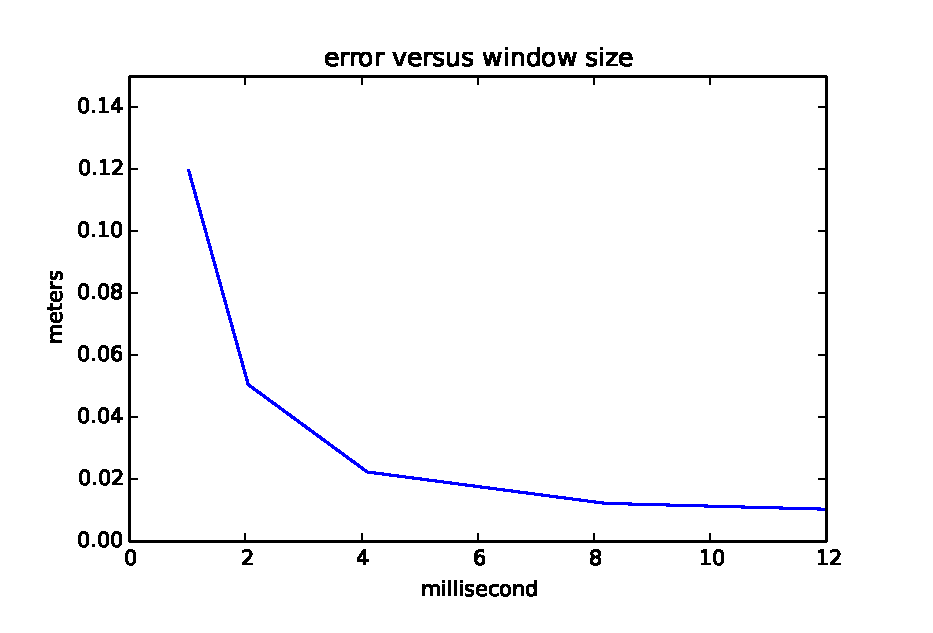
\includegraphics[width=1.0\textwidth]{error_window_size_movement.eps}
\caption{Localization error versus window size}
\label{fig:err_win_circle}
\end{figure}
Fig~\ref{fig:wn} gives an intuitive representation of how accuracy changes with window size. When window size is small ($1.02$ millisecond), the audio does not contain enough information to reliably estimate TDOA, which results in noisy localization. As window size increases, the TDOA estimation becomes more accurate and the localization converges to the shape of the ground truth circle. Fig~\ref{fig:err_win_circle} shows how the error changes with window size. The general trend is similar to that in point localization case. Error decreases as the window size increases and plateaus after it exceeds around $10$ milliseconds.

\begin{figure*}[h!]
\centering
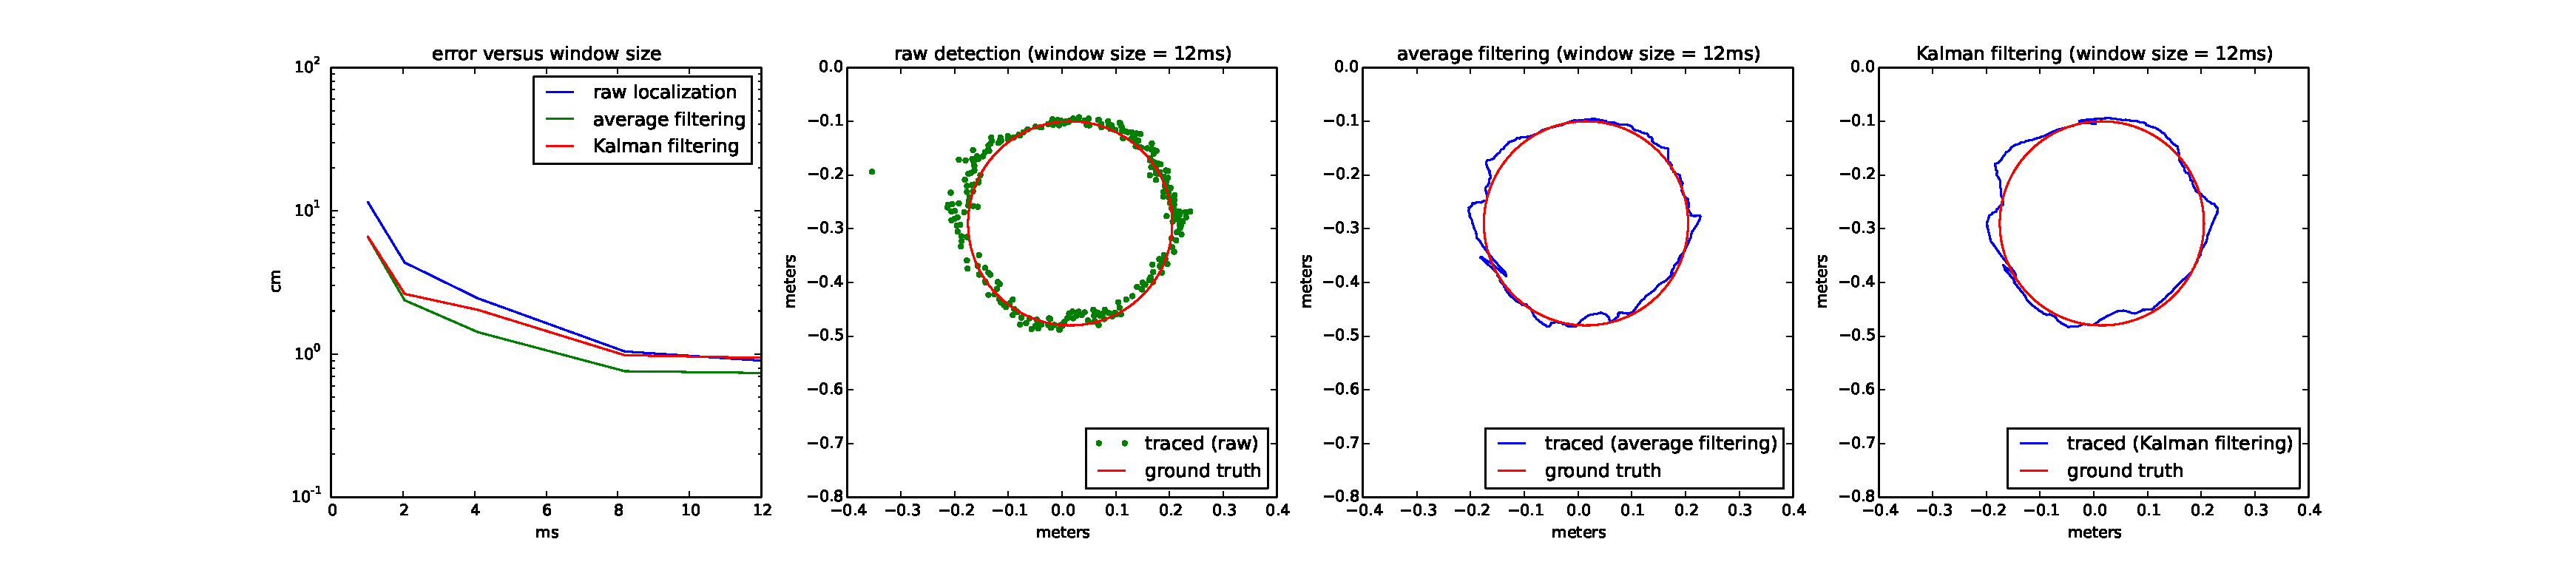
\includegraphics[width=1.0\textwidth]{trace_output_circle_wnn.eps}
\caption{white noise ($10$ cm per second)}
\label{fig:circle_wnn}
\end{figure*}

Fig~\ref{fig:circle_wnn} shows the result when white noise is used as the sound source and the source is rotated at $10$ cm per second. The top right plot in this figures shows the raw detection output with the ground truth circle overlayed on top. It shows that the array's raw output matches the underneath ground truth circle reasonably well. The average error between the localization output with its closest point on the ground truth circle is $0.9$ cm. The top left plot in the figure shows the average error with different movement filters applied as a function of window size. The error decreases as window size increases until the window size exceeds around $10$ ms. When the window size is $12$ cm, the localization accuracy is similar among raw output, Kalman filtering output and averaging filtering output. The bottom left plot shows the tracked movement for averaging filter and the bottom right filter shows the tracked movement for Kalman filtering. Kalman filtering result is smoother while the averaging tracking stays closer to the ground truth circle. Compared to the experiment in fig~\ref{fig:circle_wnf}, where the same sound source is played but rotated at a faster linear speed of $20$ cm per second, we find that the performance is equally good between these two movement speeds.

\begin{figure*}[h!]
\centering
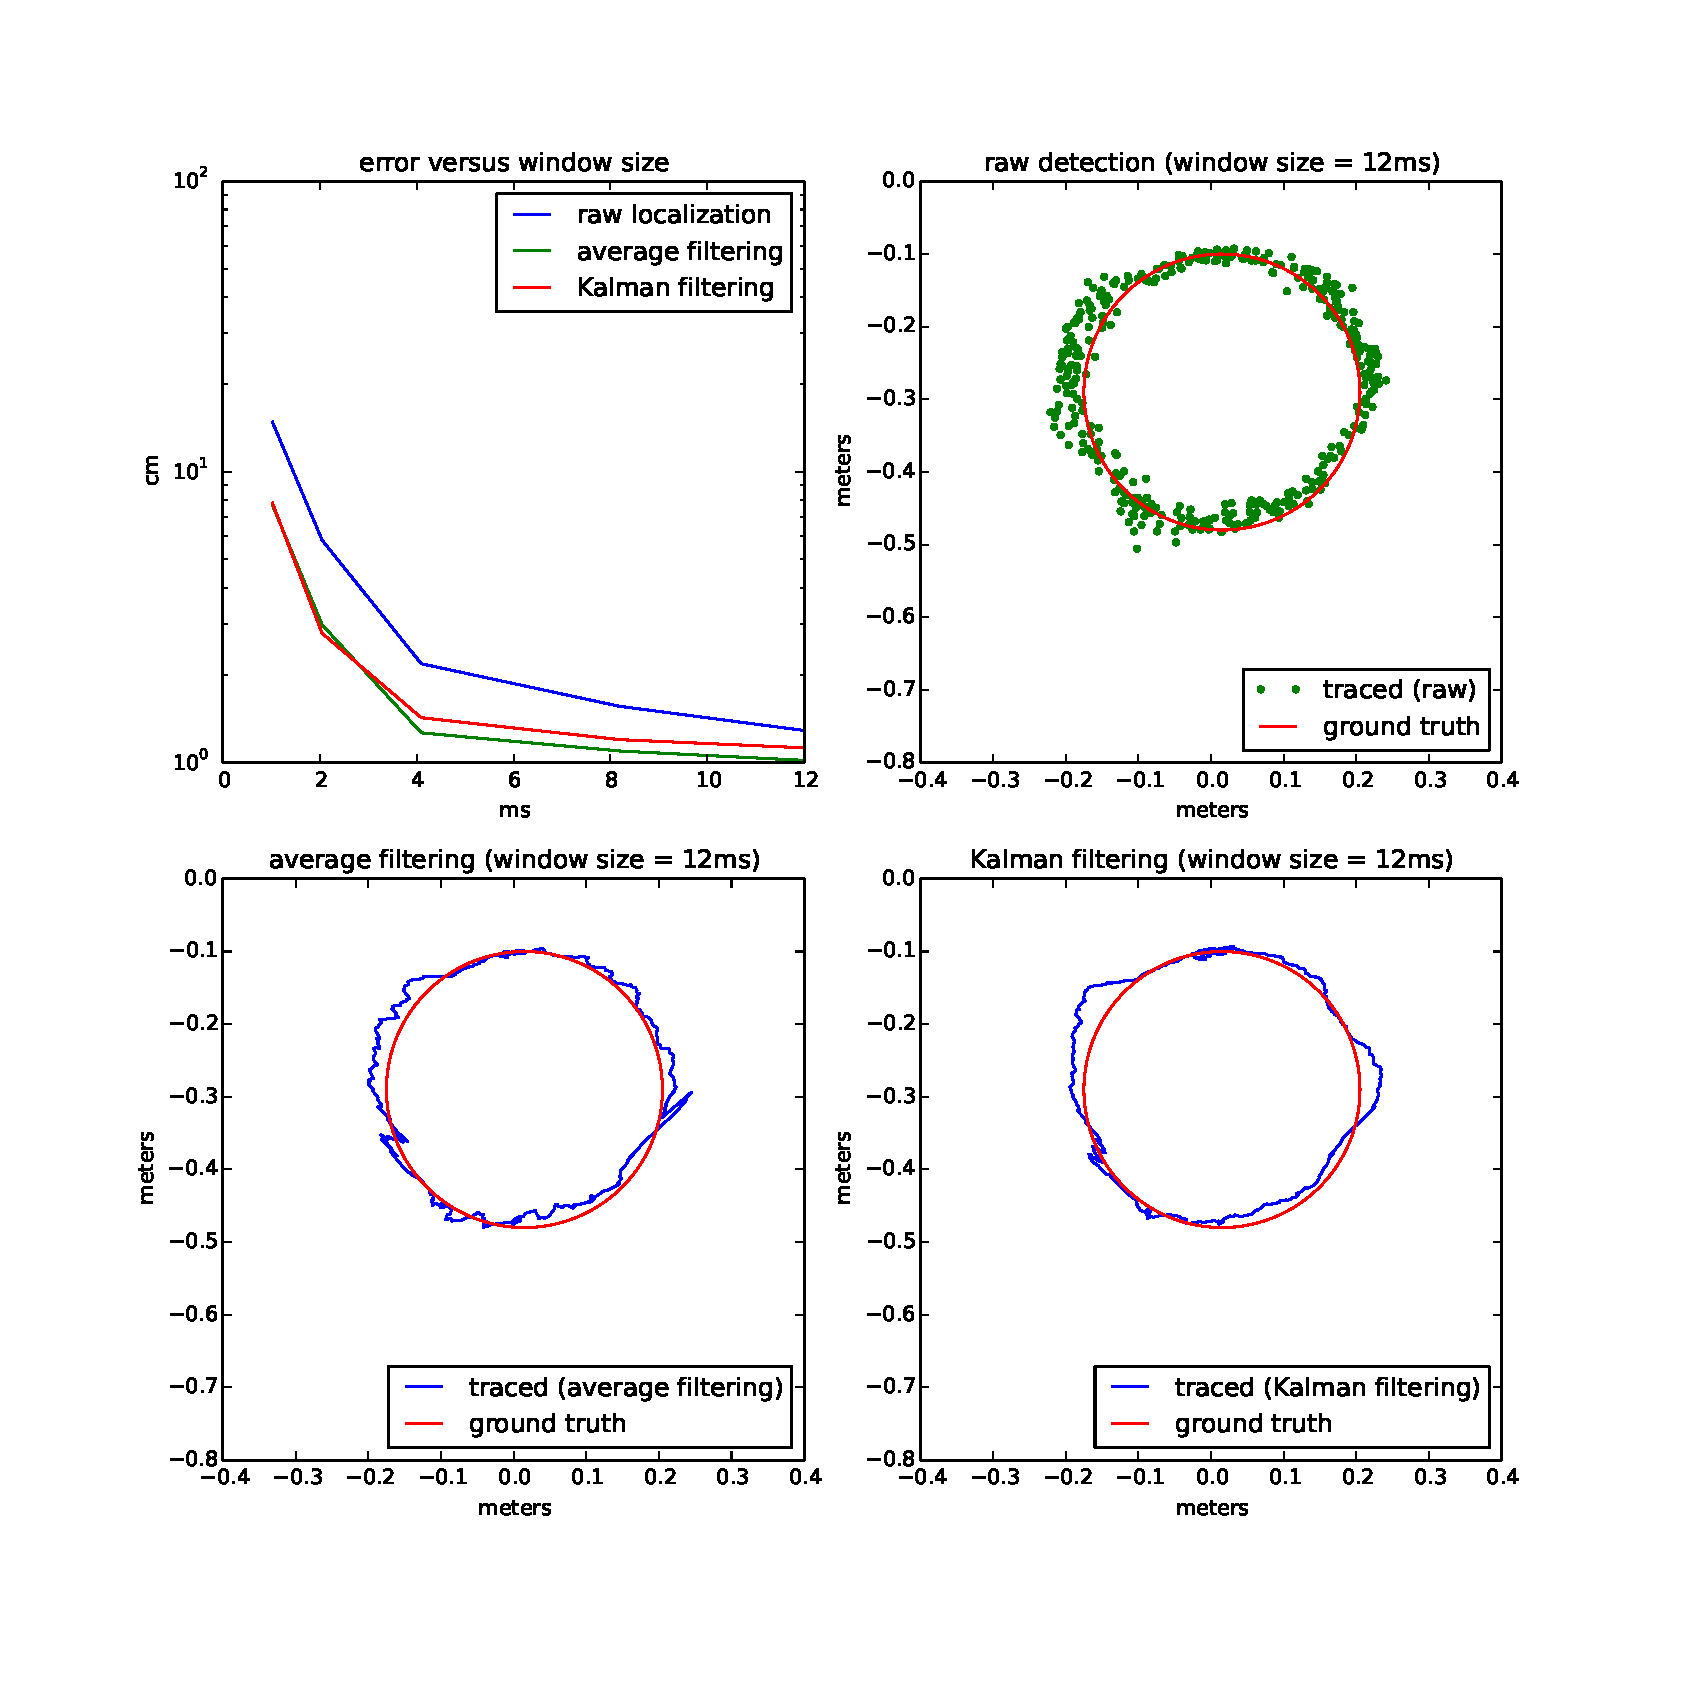
\includegraphics[width=1.0\textwidth]{trace_output_circle_man.eps}
\caption{music A ($10$ cm per second)}
\label{fig:circle_musican}
\end{figure*}

Fig~\ref{fig:circle_musican} shows the result when Music A is used as the sound source.  The top right plot shows that the array still tracks the movement well, but has a slightly larger deviation compared to that in fig~\ref{fig:circle_wnn} when white noise was used. The average localization error for Music A is $1.289$ cm. From the top left plot, it can be seen that the error still decreases with the window size. The performance improvement from raw output to Kalman filtering output is bigger than that with white noise (top left plot of fig~\ref{fig:circle_wnn}). Averaging filtering still produces lowest average error. Fig~\ref{fig:circle_musicaf} shows the result for the same sound source moved at twice the speed ($20$ cm per second). The average localization error at the faster speed is $1.291$ cm. Comparing the two experiments where music A was used as the sound source but with different movement speed, we find that the performance does not degrade as the movement speed increases from $10$ cm per second to $20$ cm per second. 

\begin{figure*}[h!]
\centering
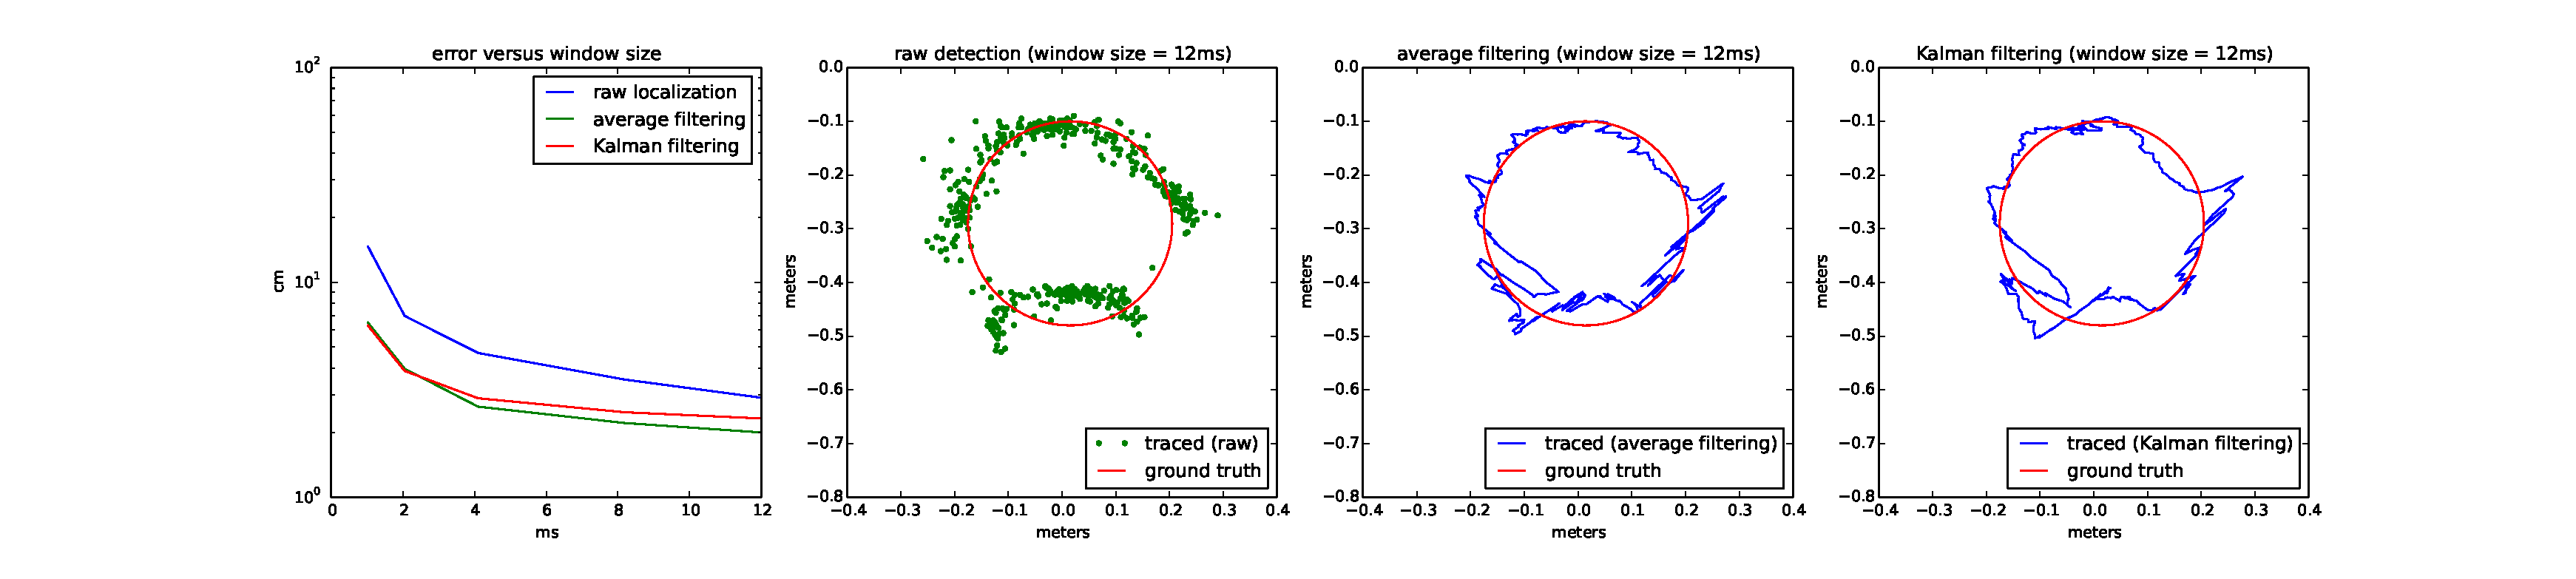
\includegraphics[width=1.0\textwidth]{trace_output_circle_mbn.eps}
\caption{music B ($10$ cm per second)}
\label{fig:circle_musicbn}
\end{figure*}

Fig~\ref{fig:circle_musicbn} shows the result when Music B is used as the sound source.  The low amplitude intervals in Music B affects the performance significantly. The average localization error is $2.9$ cm. The ``blank'' regions in the music can also be visually seen from the top right plot. The top left plot shows that the Kalman filtering still performs better than raw output. The performance improvement of Kalman filtering is similar to that with Music A. Averaging filtering produces lowest average error. Comparing to the faster movement experiment of the same sound source (shown in fig~\ref{fig:circle_musicbf}), we find that the localization error is similar between these two movement speeds.

\begin{figure*}[h!]
\centering
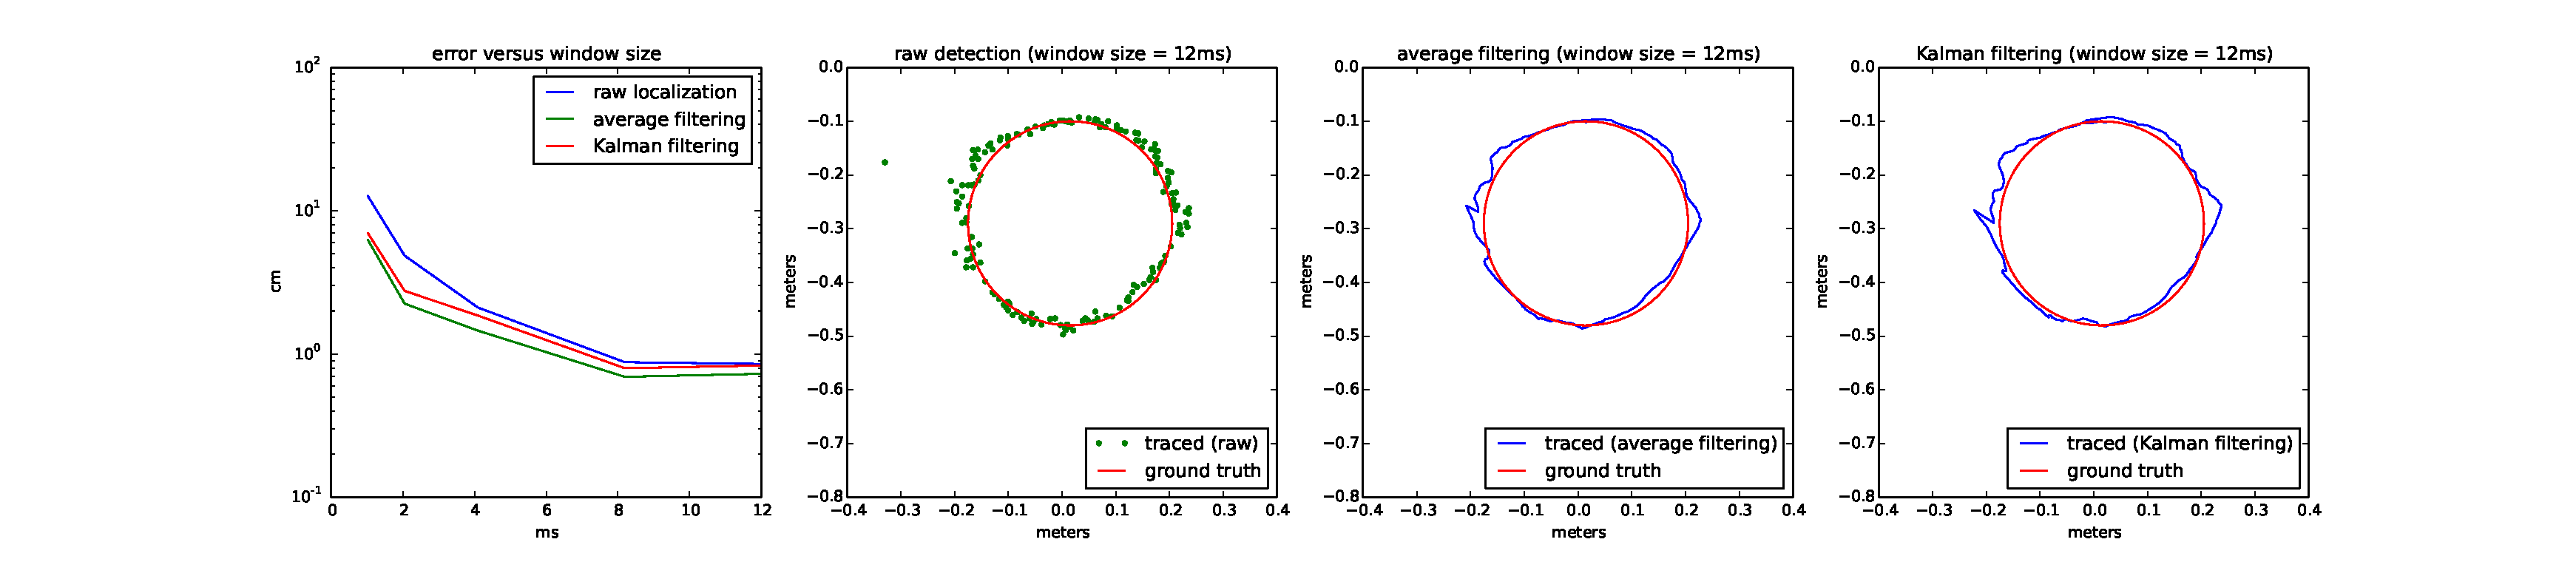
\includegraphics[width=1.0\textwidth]{trace_output_circle_wnf.eps}
\caption{white noise ($20$ cm per second)}
\label{fig:circle_wnf}
\end{figure*}

\begin{figure*}[h!]
\centering
  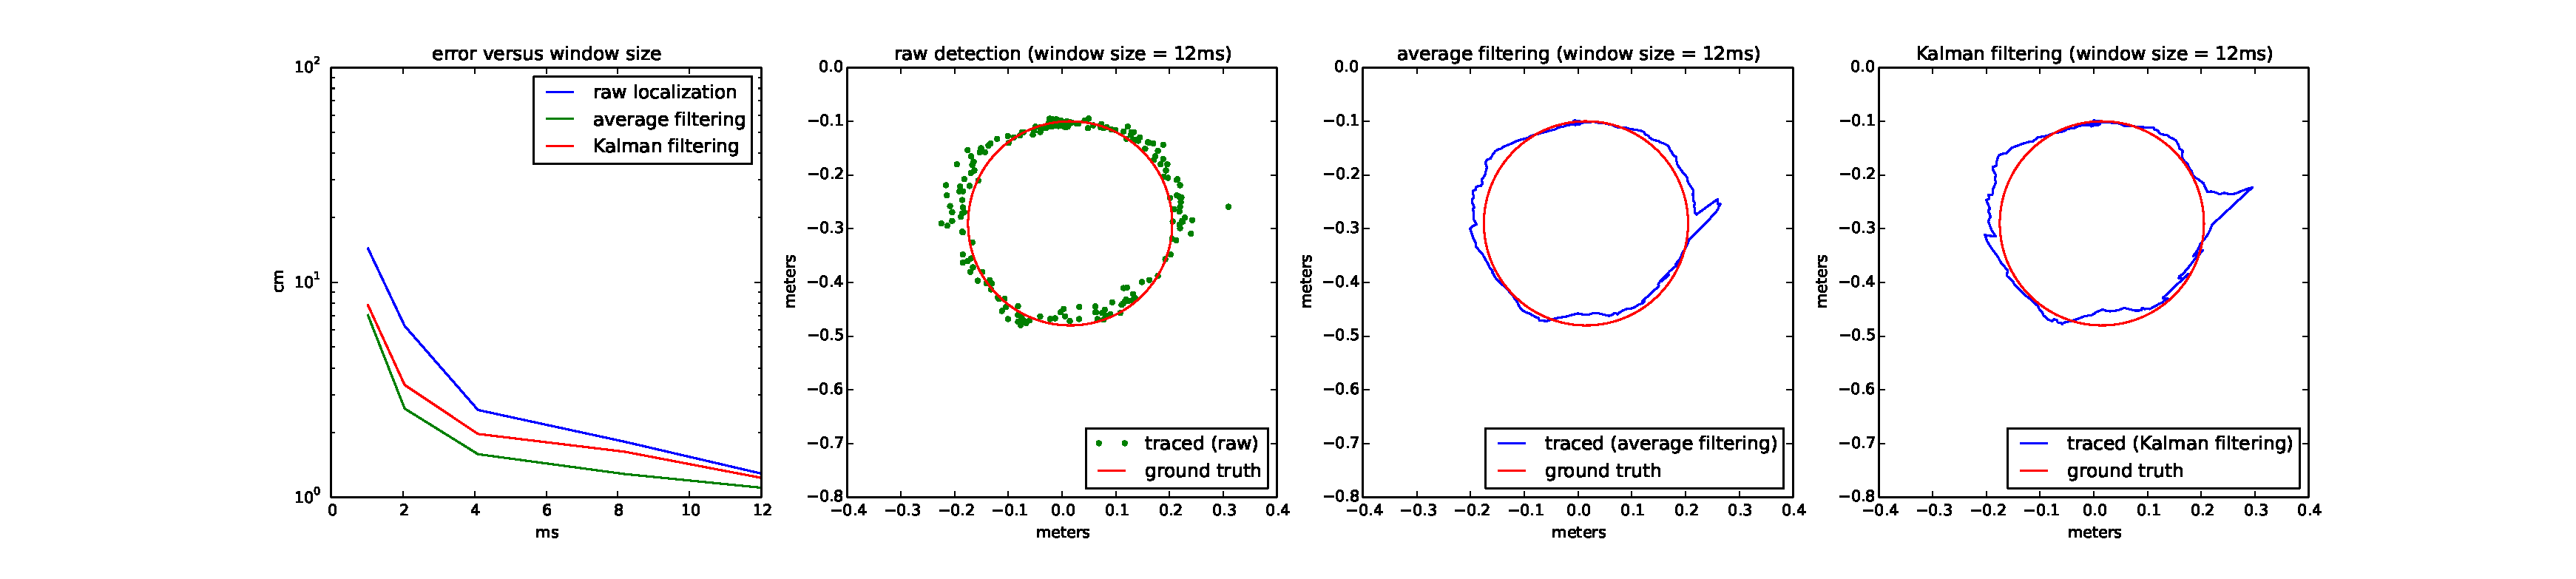
\includegraphics[width=1.0\textwidth]{trace_output_circle_maf.eps}
  \caption{music A ($20$ cm per second)}
  \label{fig:circle_musicaf}
\end{figure*}

\begin{figure*}[h!]
\centering
  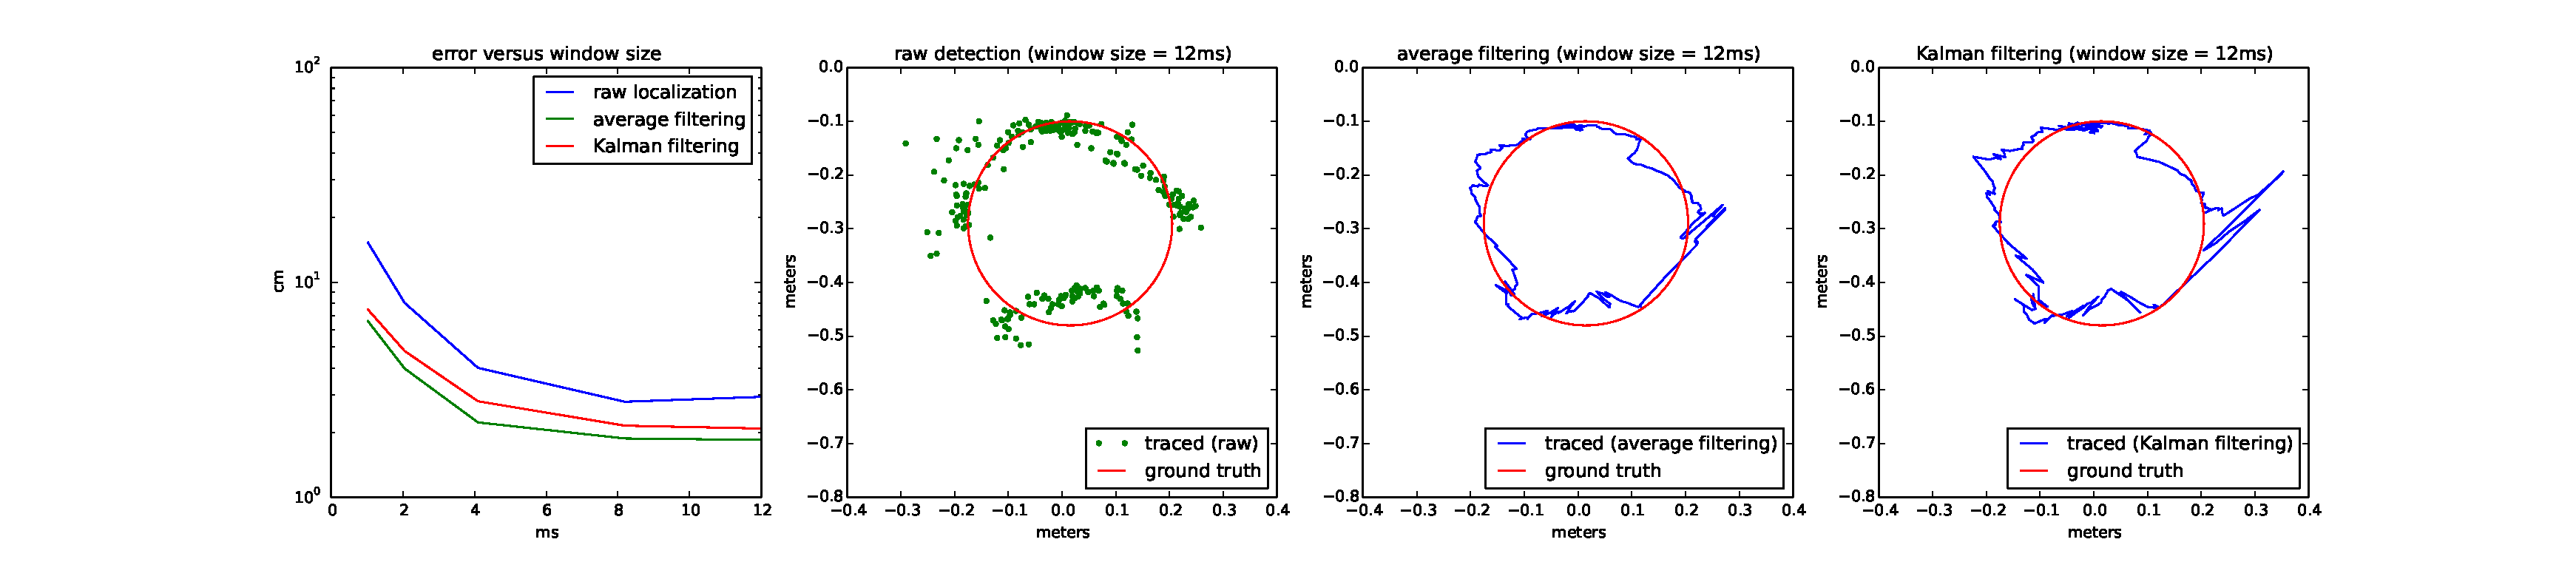
\includegraphics[width=1.0\textwidth]{trace_output_circle_mbf.eps}
  \caption{music B ($20$ cm per second)}
  \label{fig:circle_musicbf}
\end{figure*}

\subsection{Discussion}

Different prefiltering options produce very similar result. GCC\_PHAT gives slightly better accuracy, but the difference among unfiltered GCC, GCC\_PHAT and GCC\_PHAT\_SQRT is very small.

By comparing experiments at normal speed (fig~\ref{fig:circle_wnn} to \ref{fig:circle_musicbn}) with experiments at fast speed (fig~\ref{fig:circle_wnf} to~\ref{fig:circle_musicbf}), we find that the localization error does not increase when the movement speed increased from $10$ cm per second to $20$ cm per second.

When white noise is used as the audio source, Kalman filtering and raw localization produces very similar accuracy, and averaging filter gives slightly higher accuracy. However, when the audio source is changed to Music A or Music B, Kalman filtering produces better accuracy compared to raw detection, but Averaging filter still gives the best result. Looking at the smoothness of the movement path after applying different movement filters, it can be seen that raw detection has the most amount of jiggling. Kalman filter reduces the amount of jiggling from raw detection by combining past estimates with current estimates. Averaging filter has the least amount of jiggling. However, averaging filter averages detection outputs from past $0.5$ seconds, which makes the filtered output lag the real movement.

\begin{figure}[h!]
  \centering
  \begin{subfigure}[]{.48\textwidth}
    \includegraphics[width=\textwidth]{show_l.png}
    \caption{drawing letter `L'}
  \end{subfigure}
  \begin{subfigure}[]{.48\textwidth}
    \includegraphics[width=\textwidth]{show_m.png}
    \caption{drawing letter `M'}
  \end{subfigure}

  \begin{subfigure}[]{.48\textwidth}
    \includegraphics[width=\textwidth]{show_r.png}
    \caption{drawing letter `R'}
  \end{subfigure}
  \begin{subfigure}[]{.48\textwidth}
    \includegraphics[width=\textwidth]{show_c.png}
    \caption{drawing letter `C'}
  \end{subfigure}
  \begin{subfigure}[]{.48\textwidth}
    \includegraphics[width=\textwidth]{show_n.png}
    \caption{drawing letter `N'}
  \end{subfigure}
  \begin{subfigure}[]{.48\textwidth}
    \includegraphics[width=\textwidth]{show_b.png}
    \caption{drawing letter `B'}
  \end{subfigure}
  \caption{Drawing letters. Green dots represent raw localization output and the red line is the output after averaging filtering.}
  \label{fig:show_case}
\end{figure}

In figure~\ref{fig:show_case}, a few examples of drawing letters with music are presented. Each letter took around $5$ to $10$ seconds to draw, depending on the size of the letter and the speed of the movement. Green dots on the plots represent the raw localization output and the red line shows the movement output with averaging filtering (window size of $0.5$ seconds is used). The demonstrated letters are drawn with free hand, without a track guiding the movement. The accuracy is reasonably good, and each letter can be easily recognized. There is a bit of jiggling in the tracked movement. Part of the jiggling can be attributed to the noise from system output, and the rest comes from the hand movement. 

\begin{figure}[h!]
  \centering
  \begin{subfigure}[]{.48\textwidth}
    \includegraphics[width=\textwidth]{scaling_pos.png}
    \caption{randomly going through the region to collect localized $(x,y)$ data and the received volume data. The volume is kept constant}
    \label{fig:color_pos}
  \end{subfigure}
  \centering
  \begin{subfigure}[]{.48\textwidth}
    \includegraphics[width=\textwidth]{color_scaling.png}
    \caption{calculate a scaling factor for each point in the region. The scaling factor is the average of volume of the 5 closest points from the plot on the left}
    \label{fig:color_scale}
  \end{subfigure}
  \caption{Sound volume normalization}
  \label{fig:color_norm}
\end{figure}

The volume of the acoustic source can also be used to control the color of the dots painted in the above experiment.  However, the volume of the audio signal received is itself a function of the location of the audio source. Therefore, the received volume needs to be normalized. For the volume $V$ received at location $(x,y)$, we normalize it by a scaling factor $b_{xy}$. The normalized volume is $\bar{V}$:
\[
\bar{V} = \frac{V}{b_{xy}}
\]
The scaling factor $b_{xy}$ is location dependent. It is found by from calibration, which only needs to be carried out once. During calibration, a white noise sound source is moved randomly in the region with constant volume. As the source moves around in the region the calibration modules collects the source's location and received volume information. Then $b_{xy}$ is calculated by taking the volume average of $10$ closest samples from the collected data. Fig~\ref{fig:color_norm} shows and example of the volume control calibration procedure to calibrate volume information in a $60$ cm by $40$ cm region. Fig~\ref{fig:color_pos} shows how the white noise source with constant volume is moved in the region and fig~\ref{fig:color_scale} shows the scaling factor $b_{xy}$ for each point in the region by taking the volume average of $5$ closest points in fig~\ref{fig:color_pos}.

\begin{figure}[h!]
\centering
  \begin{subfigure}[]{.48\textwidth}
    \includegraphics[width=\textwidth]{color_1.png}
    \caption{drawing a strip with maximum volume}
    \label{fig:show_color_1_1}
  \end{subfigure}
  \begin{subfigure}[]{.48\textwidth}
    \includegraphics[width=\textwidth]{color_2.png}
    \caption{Drawing another strip with the volume decreased by $20\%$}
    \label{fig:show_color_1_2}
  \end{subfigure}
  \begin{subfigure}[]{.48\textwidth}
    \includegraphics[width=\textwidth]{color_3.png}
    \caption{Drawing a third strip with the volume decreased by an additional $20\%$}
    \label{fig:show_color_1_3}
  \end{subfigure}
  \caption{Drawing strips where the color of each strip is controlled by the volume of the white noise}
  \label{fig:show_color}
\end{figure}

To show how the volume acts as a color control. a simple experiment is shown in Figure~\ref{fig:show_color}. In this experiment, three stripes are drawn with the same acoustic source but different volume. The color is generated in the Hue-Saturation-Value color space where the Saturation and Value are set to $0.9$ while the hue is controlled by the volume. Figure~\ref{fig:show_color_1_1} shows the first stripe where the volume is set to the maximum and the painted color is in the red range. In fig~\ref{fig:show_color_1_2}, we painted another strip after the volume is decreased by $20$ percent. The painted color changed to the blue range after the volume is decreased. In fig~\ref{fig:show_color_1_3}, we painted a third strip where we further decreased the volume by another $20$ percent. In this final stripe, the color changed to the green range. A video demonstration is available at~\cite{demo:color}.

\begin{figure}[h!]
  \centering
    \includegraphics[width=\textwidth]{color_4.png}
    \caption{Painting a heart shape with a pop music by free hand. The color of the heart changes with the volume of the song.}
    \label{fig:show_color_2}
\end{figure}

Instead of manually varying the volume of the acoustic source, a natural extension is to use music as our acoustic source. Generally, the volume of music will vary with time and this change will be reflected by the colors drawn. In figure~\ref{fig:show_color_2}, we used a pop song as our acoustic source and painted a heart shape by free hand. The song used here is \emph{Don't Let It Break Your Heart} by \emph{Coldplay}. As can be seen from the figure, the color of the heart changes at each time instant according to the volume of the song. A video demonstration is available at~\cite{demo:color2}.




\section{Conclusion}
The conclusion goes here.




% conference papers do not normally have an appendix


% use section* for acknowledgement
\section*{Acknowledgment}


The authors would like to thank...





% trigger a \newpage just before the given reference
% number - used to balance the columns on the last page
% adjust value as needed - may need to be readjusted if
% the document is modified later
%\IEEEtriggeratref{8}
% The "triggered" command can be changed if desired:
%\IEEEtriggercmd{\enlargethispage{-5in}}

% references section

% can use a bibliography generated by BibTeX as a .bbl file
% BibTeX documentation can be easily obtained at:
% http://www.ctan.org/tex-archive/biblio/bibtex/contrib/doc/
% The IEEEtran BibTeX style support page is at:
% http://www.michaelshell.org/tex/ieeetran/bibtex/
%\bibliographystyle{IEEEtran}
% argument is your BibTeX string definitions and bibliography database(s)
%\bibliography{IEEEabrv,../bib/paper}
%
% <OR> manually copy in the resultant .bbl file
% set second argument of \begin to the number of references
% (used to reserve space for the reference number labels box)
\begin{thebibliography}{1}

\bibitem{IEEEhowto:kopka}
H.~Kopka and P.~W. Daly, \emph{A Guide to \LaTeX}, 3rd~ed.\hskip 1em plus
  0.5em minus 0.4em\relax Harlow, England: Addison-Wesley, 1999.

\end{thebibliography}




% that's all folks
\end{document}


